
\documentclass[letterpaper,openright,12pt]{book}
\usepackage[spanish]{babel} %español
%debido a que TEXstudio guarda los archivos como utf8, para escribir ñ´s y acentos directamente hay que usar utf8 como argumento de inputenc en lugar de latin1
\usepackage[utf8x]{inputenc} 

%para que enumere hasta x.x.x tanto en el indice como en el texto
\setcounter{secnumdepth}{4}
\setcounter{tocdepth}{4}
%agrega hypervinculos al pdf
\usepackage{hyperref}
%permite agregar codigo fuente
\usepackage{listings}
%insertar paginas de pdfs
\usepackage{pdfpages}
%propiedades del codigo
\lstset{language=c++,
		showstringspaces=false,
		 breaklines=true}
\usepackage{graphicx}
\usepackage{fancyhdr}
\usepackage{geometry}
\usepackage[small,bf]{caption}
\bibliographystyle{ieeetr}
%\pagestyle{fancy}

% Cambia el ancho del encabezado
\setlength{\headwidth}{16.5cm}

% Cambia el espacio para el encabezado
\setlength{\headheight}{20pt}

% Cambia el margen de los pies de figura
\setlength{\captionmargin}{20pt}

% Cambia la estructura de una página en blanco
\fancypagestyle{plain}{
\fancyhead{}
\renewcommand{\headrulewidth}{0pt}
}
\newcommand{\HRule}{\rule{\linewidth}{0.5mm}}
%esta era mi hoja de presentación
\begin{document}

%\begin{titlepage}
%\begin{center}

 %\textsc{\LARGE Universidad de Guadalajara\\}
%\textsc{\normalsize Centro Universitario de Ciencias Exactas e Ingenierías\\[3cm]}

%\Huge
%Interfaz RS-232/USB y Bibliotecas de arquitectura x86 para el control y %administración de sensores del iRobot Create

%\end{center}
%\end{titlepage}

\begin{titlepage}
\begin{center}
\vfill
{\Large  UNIVERSIDAD DE GUADALAJARA}\\[0.2cm]
\textsc{\large Centro Universitario de Ciencias Exactas e Ingenierí­as}\\[1cm]
\end{center}

\begin{center}

\includegraphics[width=5cm]{figures/escudo.png}
\end{center}

\begin{center}
\Large Interfaz y Biblioteca para el control y administración de sensores en una plataforma robótica \\[0.2cm]
\end{center}


%\vspace*{\stretch{1}} \HRule
\begin{center}
{\normalsize Proyecto de titulación que presenta}\\[0.4cm]
{\Large Omar Alejandro Rodríguez Rosas}\\[0.4cm]
{\normalsize para obtener el grado de Licenciado en Ingeniería en Computación\\[0.4cm]}
\end{center}

\pagenumbering{Roman} %las primeras páginas enumeradas en romanos

\begin{minipage}{0.5\textwidth}
\begin{center}
\emph{Directora:} \\
Dra. Nancy Guadalupe Arana Daniel
\end{center}
\end{minipage}
\begin{minipage}{0.5\textwidth}
\begin{center}
\emph{Asesora:} \\
Dra. Alma Yolanda Alanis García
\end{center}
\end{minipage}
\\[0.4cm]
%\HRule \vspace*{\stretch{2}}
\\[0.7cm]
\begin{center}
\small \textsc{2014, Guadalajara, Jalisco; México}
\end{center}
\end{titlepage}       



%una página vacía y sin numeración
\newpage
\mbox{}
\thispagestyle{empty} 

\includepdf[pages={1}]{prorroga.pdf}
\newpage
\mbox{}
%\thispagestyle{empty} 


\includepdf[pages={1}]{academico.pdf}
\newpage
\mbox{}
%\thispagestyle{empty} 

\includepdf[pages={1}]{declaratoria.pdf}
\newpage
\mbox{}
%\thispagestyle{empty} 

\includepdf[pages={1}]{dictamen.pdf}
\newpage
\mbox{}
%\thispagestyle{empty} 



\newpage

%este capitulo no se enumera ni se agrega al indice
%DEDICATORIA---------
\chapter*{}


%\begin{flushright}
%\textit{Gracias a Nestor Nápoles y a Irving Llamas por su invaluable ayuda en la codificación de este proyecto, a Edgar %Guevara por la capacitación en el uso del robot y sobre todo a mis padres por todo el apoyo que me brindaron para llegar a este lugar.}

%\end{flushright}

\tableofcontents % indice de contenidos
%salto de pagina hasta la siguiente impar
%\cleardoublepage
\newpage
%el indice aparece en la tabla de contenidos

\addcontentsline{toc}{chapter}{Índice de figuras} 
\listoffigures 

%\cleardoublepage
%\addcontentsline{toc}{chapter}{Índice de tablas}
%\listoftables % indice de tablas



\underline{\underline{}}\chapter{Introducción}
\pagenumbering{arabic}

Desde sus inicios a principios de la decada de 1960, la importancia de la Robótica y los Sistemas Inteligentes como áreas de investigación ha crecido de manera exponencial de tal forma que hoy en día, ambas disciplinas juegan un papel de gran importancia en campos tan diversos como la educación, la salud, la manufactura, el cuidado del hogar, el control de inventarios , la seguridad, el rescate, operaciones militares, entre otros \cite{lazinica}.\\
Como era de esperarse, este crecimiento se vió reflejado en la industria como un incremento en la demanda de profesionistas capacitados en dichas disciplinas\cite{stites}. Sin embargo, en años recientes diversas universidades de los Estados Unidos y la Unión Europea han experimentado una disminución en el interés por carreras afines \cite{vegso}\cite{davidson} lo que sugiere  dificultades para satisfacer esta demanda a mediano plazo.\\
Buscando subsanar por lo menos de manera parcial esta brecha en la oferta-demanda educacional, estudios recientes han demostrado cómo el estudio de la robótica en etapas tempranas de la educación (digase preparatoria) ayuda a disminuir el rechazo hacia las ciencias matemáticas, de la ingeniería y la computación que muchos alumnos perciben como difíciles, altamente demandantes y en general indeseables\cite{salamon}.\\
Si bien es cierto que la robótica forma parte del mapa curricular en muchas universidades, el trabajo con robots reales supone una tarea abrumadora para la mayoría de los estudiantes a nivel de licenciatura lo que sumado a los altos costos del equipo de laboratorio lo convierte en un privilegio reservado generalmente para los investigadores y alumnos de posgrado\cite{challinger}.\\
Por fortuna, en años recientes se han lanzado al mercado diferentes plataformas, frameworks y APIs tales como los Lego Mindstorms, los MIT Handyboards, los Rug Warriors, entre otros \cite{goldweber} proveyendo a estudiantes y profesores de herramientas para lograr una introducción sencilla a temas básicos de robótica y una transición suave hacia tópicos más complejos. Este tipo de plataformas han sido bien recibidas en gran medida gracias a su bajo precio, su robustez y su corto ciclo de desarrollo haciendolos ideales para el trabajo en proyectos de licenciatura o incluso preuniversitarios.\\
Las nuevas posibilidades ofrecidas por esos sistemas de bajo costo han sido exploradas a profundidad en un gran número de investigaciones educativas y han probado ser un recurso invaluable para el salón de clases ya que ayudan a los estudiantes a desarrollar habilidades como la descomposición de problemas, la creación de procedimientos, el trabajo multidisciplinario en equipo\cite{goldweber} y diseño de software en un ambiente controlado y divertido  \cite{salamon} volviendolos conscientes del equipo disponible en los laboratorios y brindandoles la confianza, conocimientos y experiencia necesarios para proponer futuros trabajos de posgrado\cite{challinger}.\\
En el caso concreto del Laboratorio de Sistemas Inteligentes en el Centro Universitario de Ciencias Exactas e Ingenierías de la Universidad de Guadalajara, la experiencia con este tipo de sistemas comenzó en el año 2010 con la adquisición de 2 robots Qbot (figura \ref{fig:qbot}), un modelo comercializado por la empresa canadiense Quanser y basado en la plataforma Create\textsuperscript{\textregistered} de iRobot (ver \ref{sec:iRobot}) que añade a esta última cinco sensores de distancia infrarrojos, 3 ultrasónicos y una cámara web que le permiten una mayor flexibilidad y lo hacen apto para proyectos más avanzados. Además, el control del robot y la adminisracion de sus sensores puede llevarse a cabo mediante Matlab/Simulink a través  QuaRC -el bloque control para sistemas en tiempo real de Quanser- OpenCV, QMRFC, Roomba, entre otros. \cite{huq}\\

\begin{figure}
\begin{center}
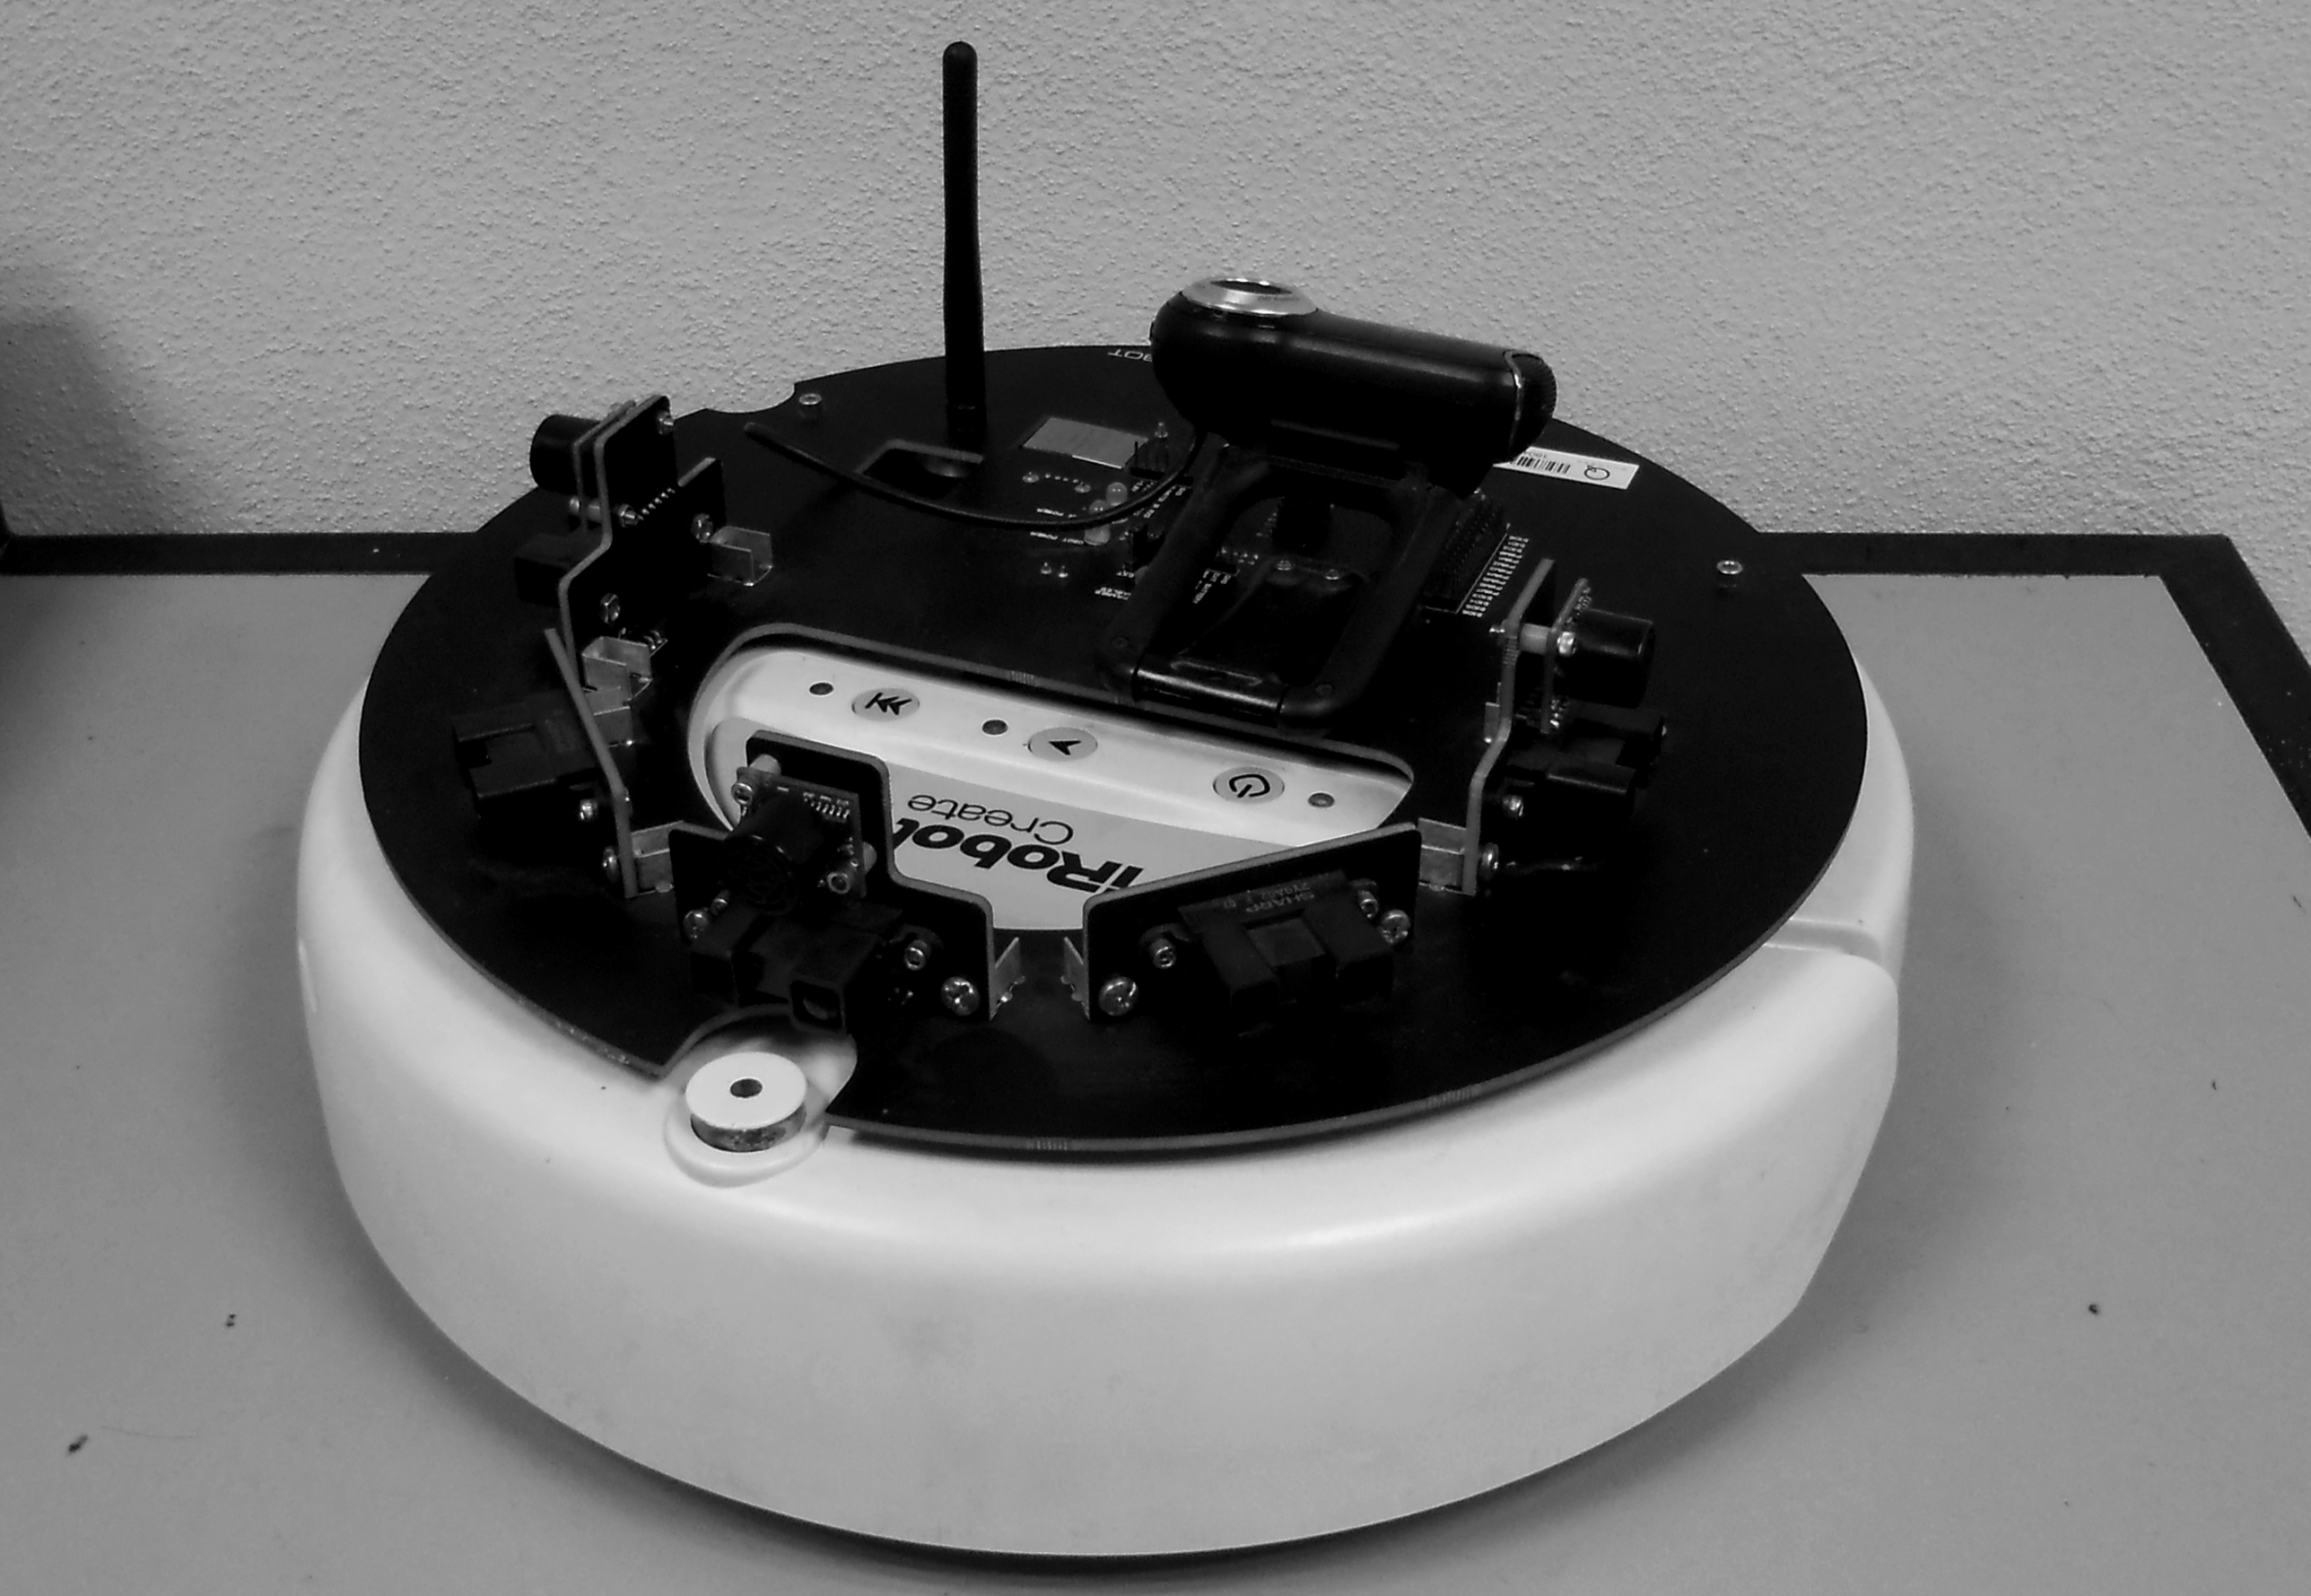
\includegraphics[width=0.8\textwidth]{figures/qbot.jpg}
\caption{El Qbot de Quanser}
\centering
\label{fig:qbot}
\end{center}
\end{figure} 

Sin embargo, a pesar de que el Qbot permite el prototipado rápido de muchas aplicaciones también posee serios inconvenientes que lo hacen poco apropiado para el desarrollo de proyectos más formales. El primero de ellos es la comunicación inalámbrica por medio del protocolo TCP que se utiliza como forma de contacto principal entre la PC y el robot, el cual es conocido por generar considerables retardos debidos a las limitaciones de ancho de banda y al preprocesamiento de seguridad adicional propios del protocolo\cite{nilsson}. El segundo tiene que ver con los problemas inherentes al uso de Matlab/Simulink para el control de sistemas en tiempo real como la inflexibilidad del código\cite{sjostedt} y el no determinismo temporal\cite{henriksson} además de la naturaleza considerablemente más lenta de los lenguajes de programación interpretados (comparados con otros lenguajes compilados como c/c++).\\
Estas consideraciones nos llevaron a buscar otras altenativas que permitieran un desarrollo más eficiente y flexible. El primer enfoque para ello fue interceptar el proceso de transmisión de datos mediante un sniffer TCP y aplicar ingeniería inversa a este proceso con la finalidad de sustituir el código generado en Simulink por el propio. Aunque factible, dado que los procedimientos específicos de comunicación PC-robot del Qbot son de código cerrado y no documentados, esta idea fue descartada debido a la cantidad de trabajo que implicaba, las posibles implicaciones legales respecto al uso de licencias y a que, en el mejor de los casos solo se resolvía el segundo de los dos problemas anteriormente presentados pero no el desempeño general del sistema entorpecido por la comunicación inalámbrica.
Por ello, se optó por retirar el hardware de control de sensores y comunicación del Qbot construido alrededor de una microcomputadora Gumstix (de arquitectura ARM) y sustituirlo por un diseño de hardware a medida directamente sobre el iRobot Create\textsuperscript{\textregistered} que constituye la base del Qbot.\\
A pesar de que existen algunas bibliotecas de control para el iRobot Create\textsuperscript{\textregistered} (ver \ref{sec:iRobot}) ninguna de ellas satisface del todo las necesidades de los trabajos de investigación del laboratrio.\\
Por esta razón, el objetivo primordial de este trabajo es desarrollar la biblioteca UDG\_Create, un \emph{framework} integral con un funcionamiento a bajo nivel pero con funciones y abstracciones de hardware de alto nivel para el manejo del robot que mediante el uso de c++ como lenguaje de programación principal y un sistema operativo basado en linux permita un desarrollo flexible y eficiente eliminando prácticamente en su totalidad los costos de licencias de software. Además, gracias su implementación alrededor de un sistema de arquitectura x86, se expanden aún más las capacidades del iRobot Create\textsuperscript{\textregistered} aumentando considerablemente su poder de computo y su compatibilidad con un sinfín de aplicaciones y dispositivos de hardware diseñados para los procesadores con este tipo de set de instrucciones.\\


%\section{Objetivos}

%\section{Justificación}

%\section{Definición del problema}
% %----------------------------------- % %
\chapter{Marco teórico}
\section{El iRobot Create\textsuperscript{\textregistered}}
\label{sec:iRobot}
Este robot, basado en la aspiradora robótica autónoma Roomba (ver \ref{fig:create}) y comercializado por la empresa iRobot fue concebido como un kit de desarrollo que permite la implementación de algoritmos y diseño de nuevos comportamientos de manera sencilla manteniendo los aspectos mecánicos y electrónicos de la operación transparentes al usuario\cite{irobotm}. Posee 10 modos de demostración que pueden utilizarse directamente de fábrica, pero también puede ser manejado por una PC o microcontrolador a través de un puerto serial dedicado con un conector mini-DIN 7 o mediante un conector DB-25.\\
Está provisto de 20 sensores entre los que se incluyen detectores de bordes, un receptor infrarrojo, un parchoques de 4 estados, motores independientes para cada una de sus dos ruedas móviles, tres LED's indicadores, tres botones programables, una salida digital de niveles TTL de 3 bits y 3 salidas para PWM que permiten la adición de electrónica adicional como brazos robóticos o actuadores\cite{irobotopen}\cite{irobotp}.\\
\begin{figure}
\begin{center}
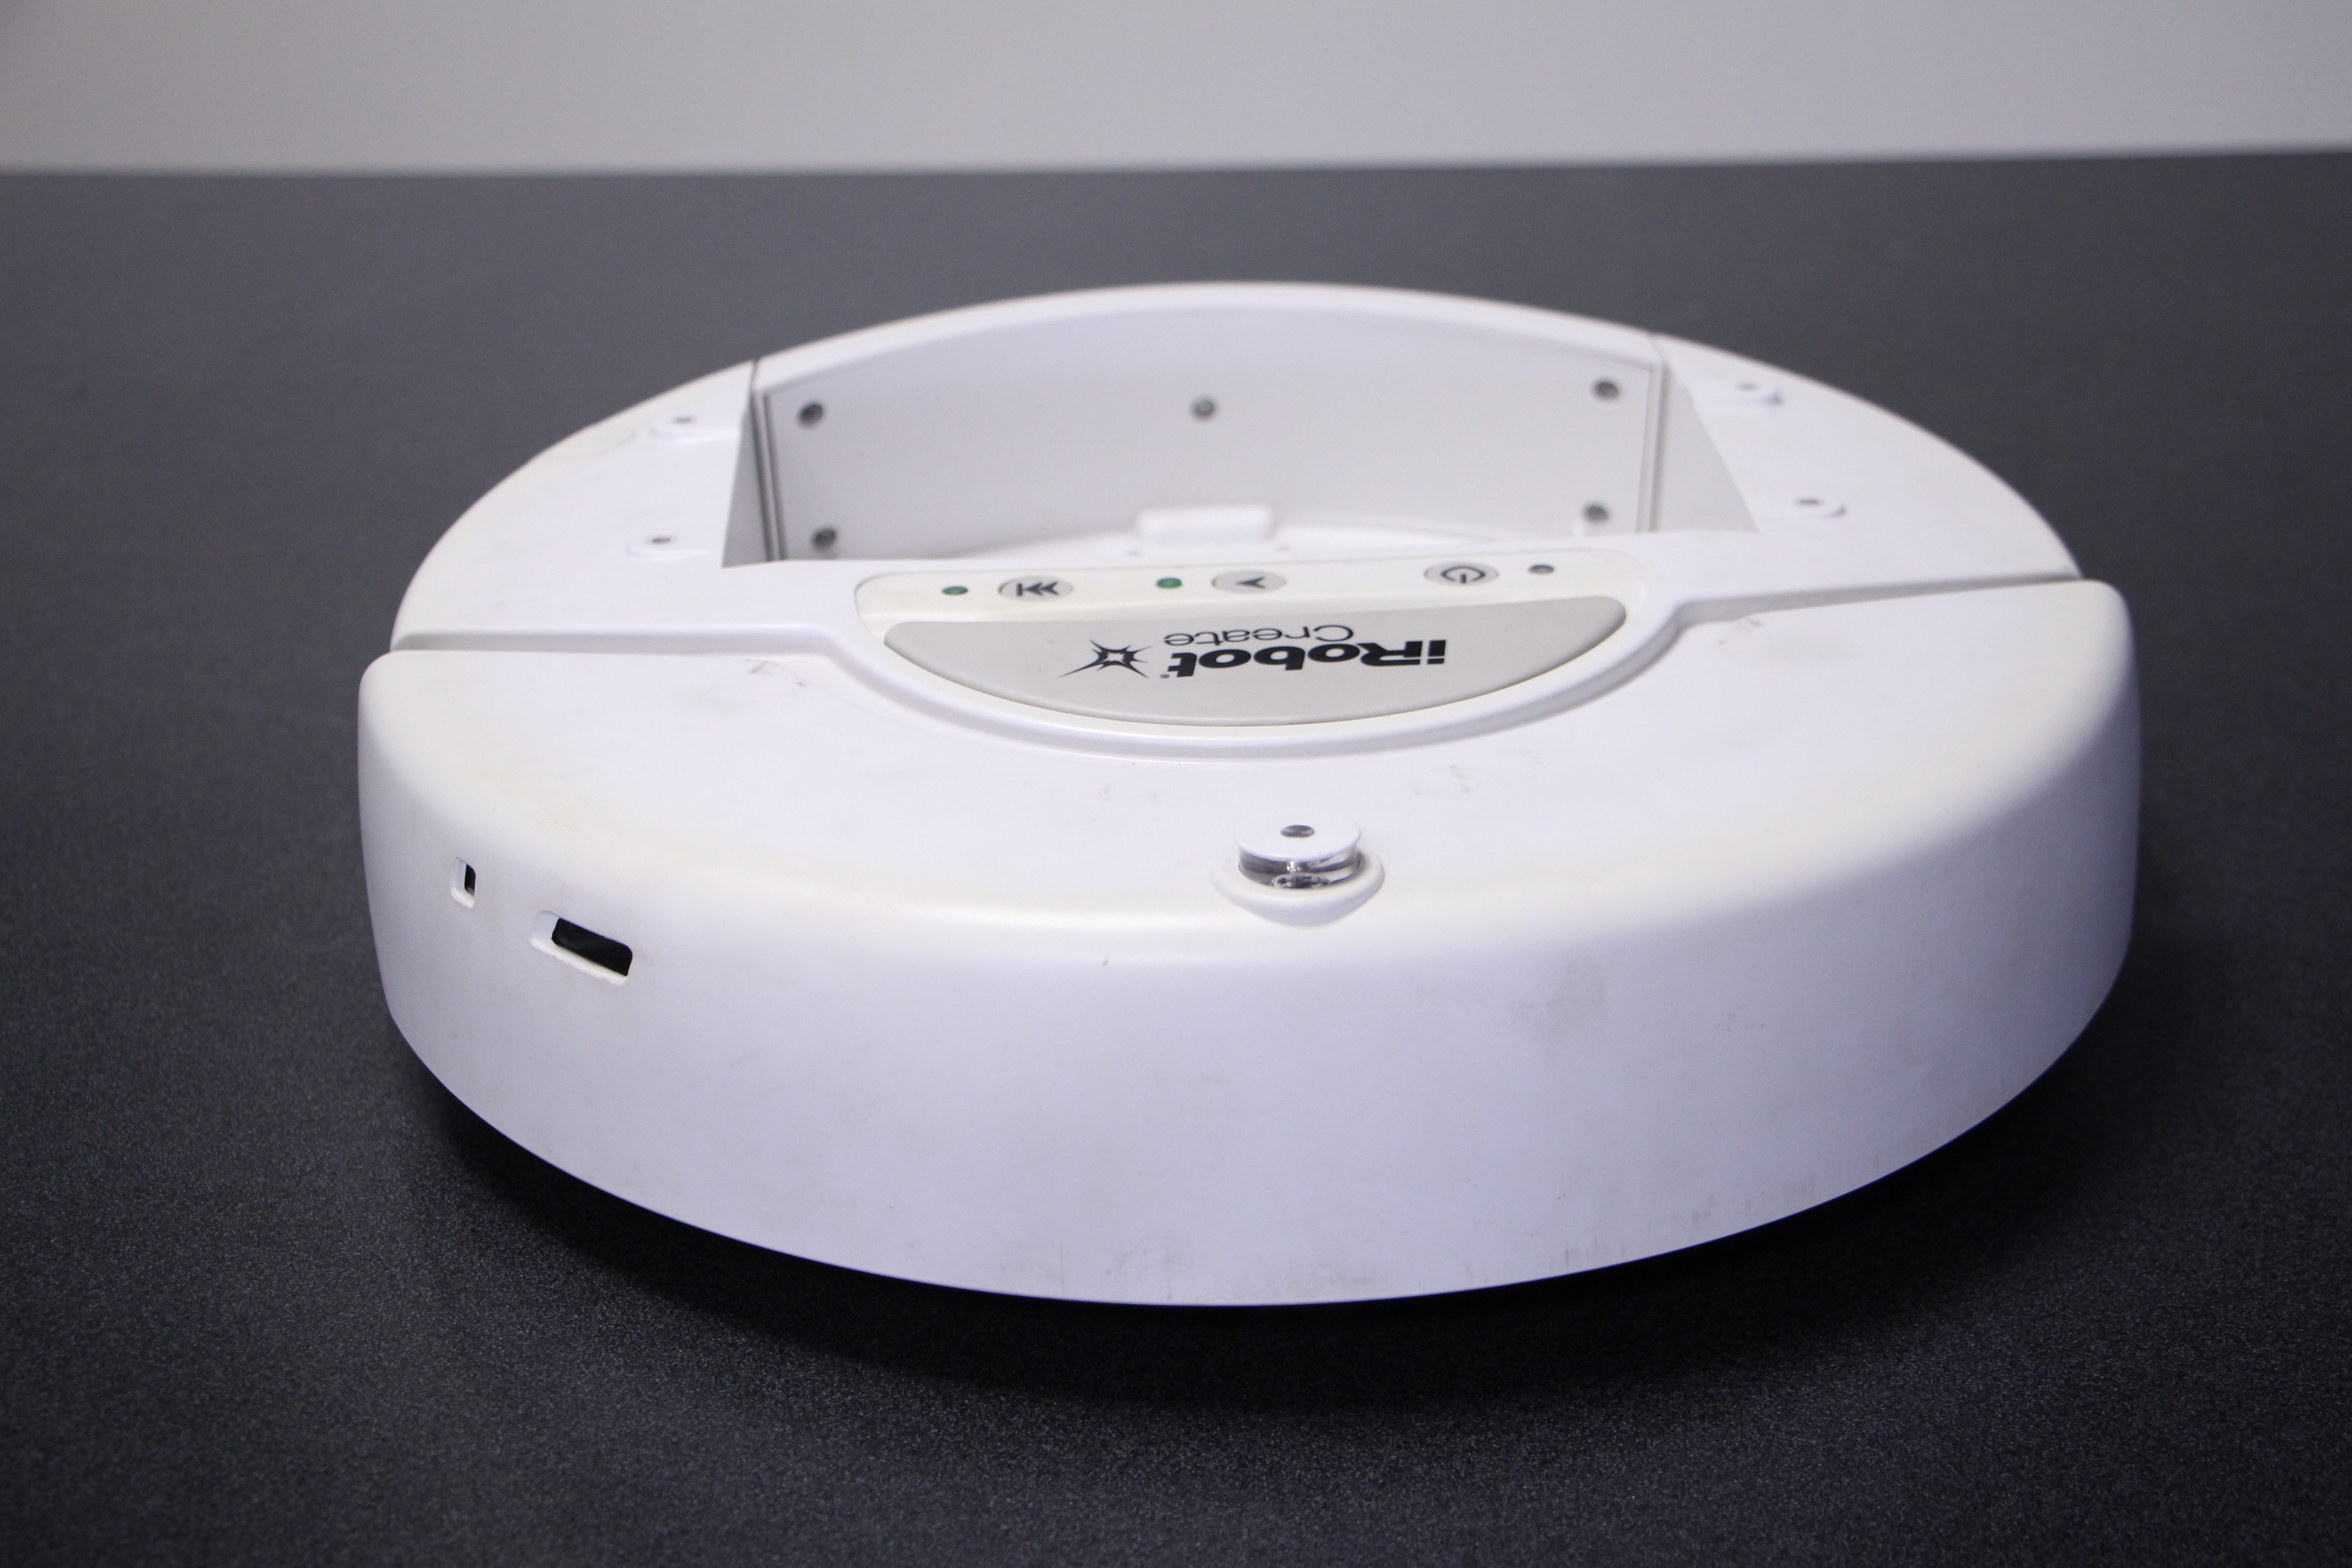
\includegraphics[width=0.8\textwidth]{figures/create.jpg}
\caption{El Create\textsuperscript{\textregistered} de iRobot}
\centering
\label{fig:create}
\end{center}
\end{figure} 
En el ámbito académico este robot ha sido utilizado como base para investigaciones en temas como telepresencia \cite{lee}, mapeo tridimensional \cite{ellaithy}\cite{saenz} y localización \cite{housten}\cite{kuipers} demostrando sus capacidades como una plataforma asequible, robusta y fácil de usar.\\
Como muestra de su popularidad cabe mencionar la presencia de drivers, modelos de simulación y bibliotecas de control en importantes entornos como The Player Project \cite{pharos}, Universal Real-time Behavior Interface (URBI) \cite{urbiforge}, Microsoft Robotics Studio \cite{microsoft}, Webots \cite{microsoft} y el Robot Operating System (ROS)\cite{rosorg}.\\




\section{El estándar RS-232}
El estándar para comunicación serial RS-232, también conocido como EIA/TIA RS-232C, define el cableado, conectores, niveles de voltaje, temporización de señales y prótocolo de intercambio de información entre un Dispositivo Terminal de datos (DTE) y un Dispositivo de Comunicación de datos (DCE) mediante una transmisión serial de datos binarios.\\
Una implementación completa del estándar utiliza un conector de 25 terminales DB-25, pero también son comunes versiones reducidas de 9 e implementaciones mínimas de 4, en los que se asigna una función y posición a cada terminal (ver figura \ref{fig:232pinout}). La comunicación es asíncrona (pero síncrona a nivel de bit) en modos simplex, half duplex y full duplex.\\
A pesar de no estar considerado en la especificación del estándar, es muy común conectar dos dispositivos DTE (por ejemplo dos computadoras personales) directamente entre ellos en lo que se denomina una conexión de módem nulo. Para lograrlo se utilizan por lo general cables cruzados cuya organización interna suele variar de una implementación a otra.\\
Para la transferencia de datos binarios se establecen niveles de voltaje en lógica negativa con amplios margenes de tolerancia que le brindan una gran robustez. Durante la transmisión, un 0 binario será representado mediante un voltaje de entre +5v y +15v mientras que un 1 se enviará con un nivel de entre -5v y -15v. Para la recepción estos niveles varían ligeramente ya que un voltaje de entre +3v y +13v se interpretará como un 0 binario y entre -3v y -13v como un 1.\\
El protocolo de comunicación señala que, para la transmisión, en estado ocioso se envían bits en nivel alto de manera continua. El comienzo de la comunicación se indica mediante un bit de inicio que es siempre un nivel bajo segudio de los entre 5 y 8 bits de datos. El fin de la transmisión se especifíca mediante un nivel alto que debe durar por lo menos 100$\mu$s para después iniciar una nueva transmisión o volver al estado ocioso.\\
La recepción comienza con el dispositivo esperando a que la línea pase a un nivel bajo. Al ser detectado , el receptor esperá 51$\mu$s de manera que se encuentre a la mitad del bit para descartar que el cambio de nivel haya sido ocasionado por ruido. Posteriormente esperará 104$\mu$s más hasta encontrarse a la mitad del primer bit de datos. El resto de las lecturas se hacen de la misma manera hasta encontrar el bit de parada (ver \ref{fig:232communication})\cite{omega}.\\
\begin{figure}
\begin{center}
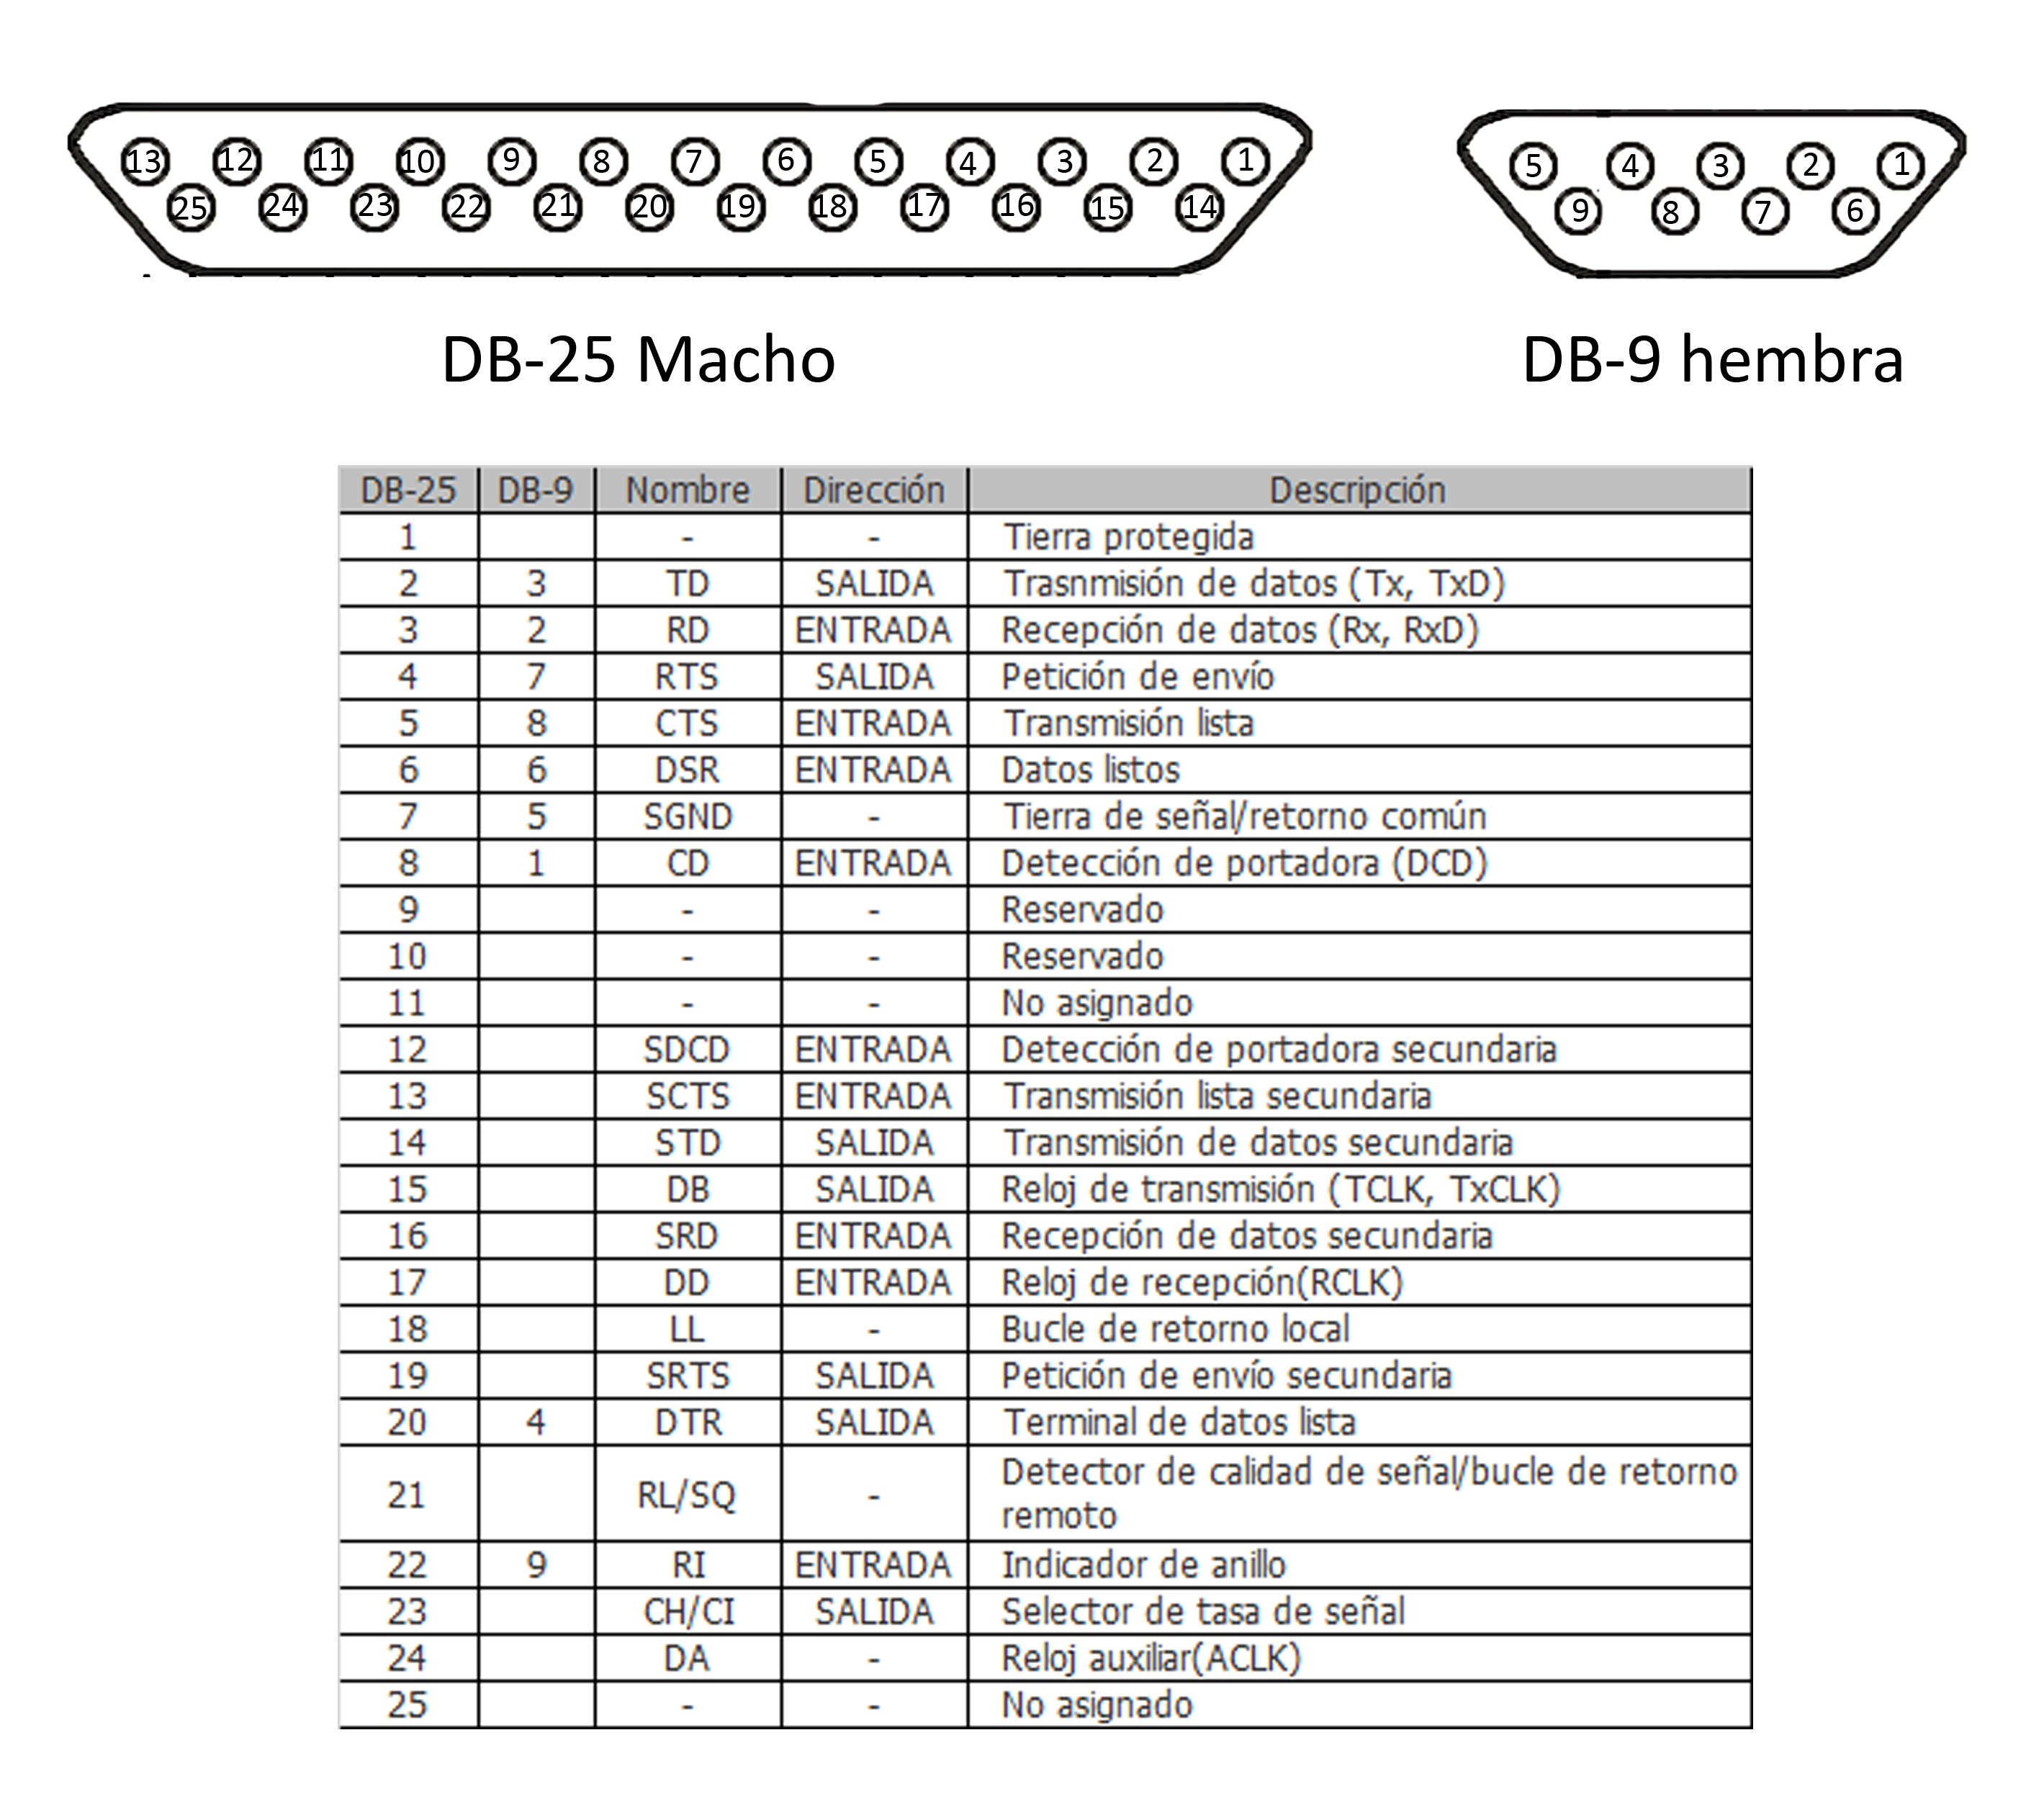
\includegraphics[width=0.8\textwidth]{figures/terminalesrs232.png}
\caption{Distribución de pines en el estándar RS-232 para los conectores DB-9 hembra y DB-25 macho}
\centering
\label{fig:232pinout}
\end{center}
\end{figure} 

\begin{figure}
\begin{center}
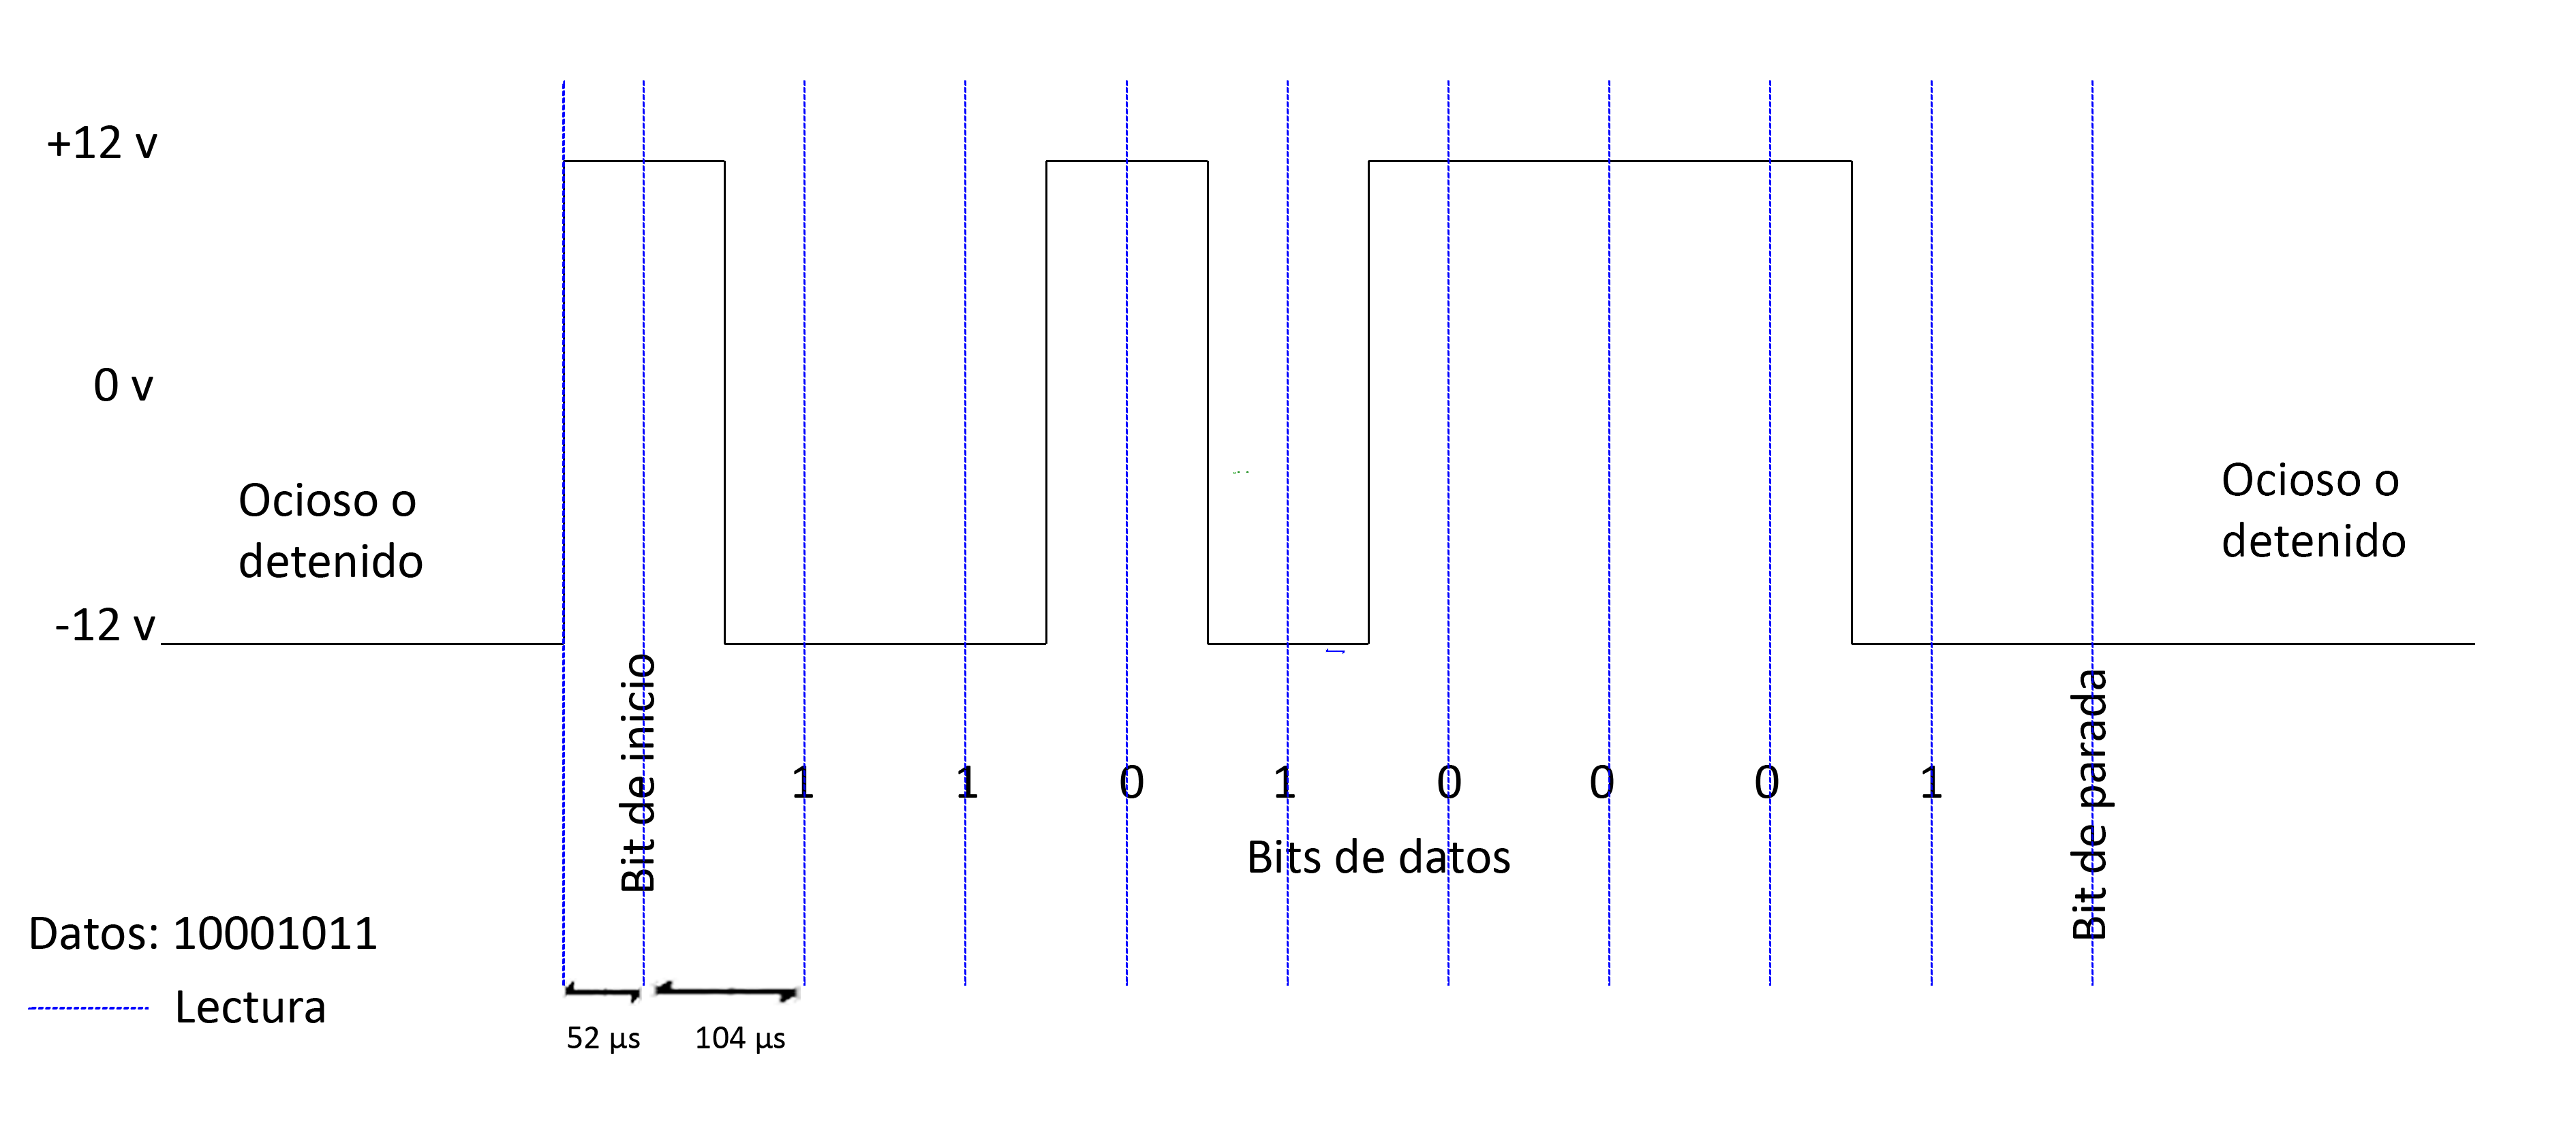
\includegraphics[width=0.8\textwidth]{figures/comunicacionrs232.png}
\caption{Protocolo de comunicación mediante RS-232 para una transmisión de 8 bits de datos sin bit de paridad}
\centering
\label{fig:232communication}
\end{center}
\end{figure} 
\section{El estándar USB 2.0}
El bus universal en serie (USB por sus siglas en inglés) es un estándar que define el cableado y protocolos de comunicación entre una computadora y sus periféricos. La especificación original publicada por primeara vez en 1996 buscaba facilitar la interconexión entre las computadoras personales y los telefonos, brindar flexibilidad y reconfigurabilidad a los sistemas de computo mediante software amigable y hardware \emph{plug-and-play} paliando la indisponibilidad, en aquel entonces, de puertos bidireccionales de bajo costo y velocidad media no ligados a un dispositivo en particular.\\
Un tiempo después, en el año 2000, el aumento en la velocidad de procesamiento de las computadoras y las crecientes capacidades de los periféricos motivaron la definición de una nueva especificación USB 2.0 en la que se aumentaba la tasa máxima de transferencia del bus de 12Mb/s a 480Mb/s proporcionando soporte para voz, audio y video y agregando algunas clases de dispositivos, pero manteniendo a la vez el bajo costo, flexibilidad y compatibilidad total con versiones anteriores.\\
Esta especificación, USB 2.0, es la que se utiliza a lo largo de este trabajo.\\


\subsection{Protocolo de comunicación USB}
Un sistema USB está compuesto por un \emph{host} principal, concentradores y dispositivos conectados con una topología de estrella escalonada (ver \ref{fig:usbtopology}) en la que el centro de cada estrella es un concentrador y el resto de las conexiones son entre el host principal y un concentrador  o dispositivo, o bien, entre un concentrador y otro concentrador o dispositivo.\\
Debido a los retrasos de propagación del cableado y las limitaciones de tiempo que establece el propio protocolo, el número de niveles en la topología está limitado a siete incluyendo al host, además de que el último escalón no puede contener un concentrador o dispositivo compuesto.
Los tipos de transferencias de datos definidas en el estándar son:\\
\textbf{Transferencias de control}: Se utilizan para configurar dispositivos recién conectados o par implementar funcionalidades muy específicas.\\
\textbf{Transeferencias por volumen}: Se refiere a grandes cantidades de datos secuenciales, por ejmplo, los provenientes de una cámara digital.\\
\textbf{Transferencias por interrupción}: Están generalmente asociadas con funcionalidades de notificación de eventos que se presentan en cualquier momento.\\
\textbf{Transferencias Isócronas}: Consiste en la creación, entrega y consumo de datos en tiempo real a una tasa constante. Se utiliza para aplicaciones sensibles al tiempo como lo es la transmisión de voz. Algunos mecanismos de seguridad e integridad de datos como la retransmisión no se aplican a este tipo de transferencia.\\

\begin{figure}
\begin{center}
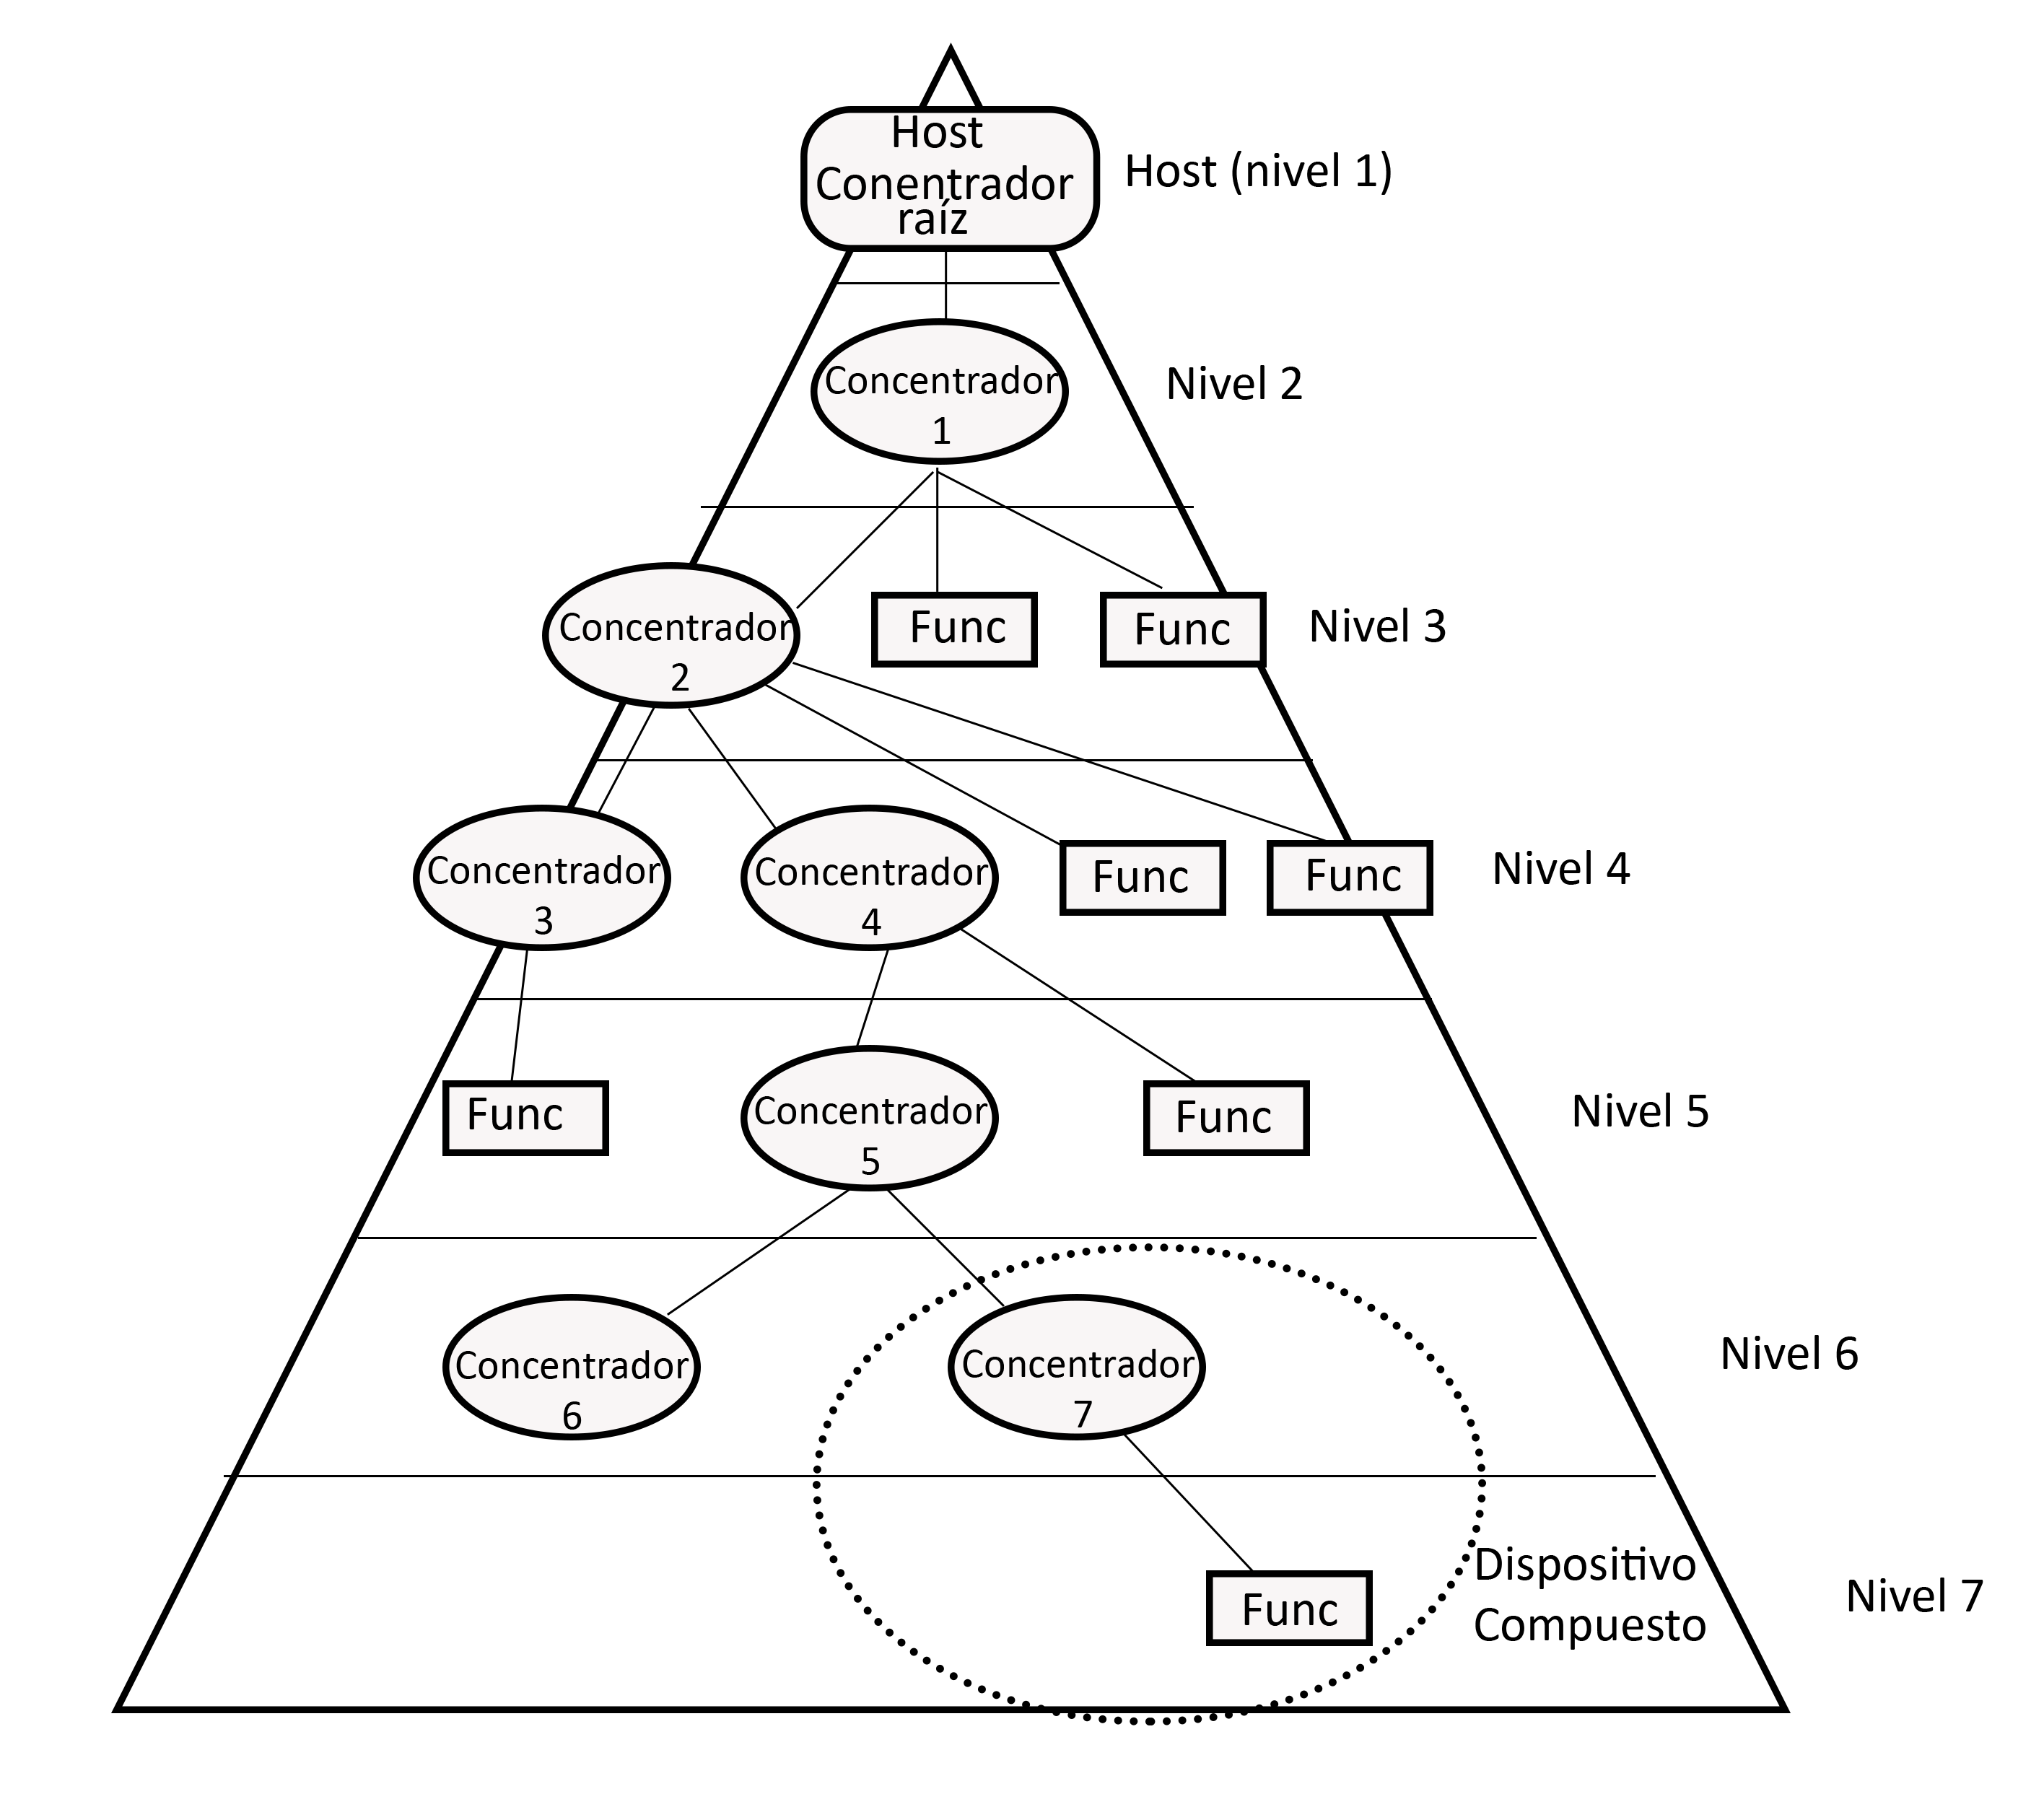
\includegraphics[width=0.8\textwidth]{figures/topologiaUSB.png}
\caption{Topología de bus USB}
\centering
\label{fig:usbtopology}
\end{center}
\end{figure} 

\subsection{Conexión, desconexión y enumeración de dispositivos}
Dado que se permite la conexión y desconexión de dispositivos en cualquier momento, una enumeración de estos y sus respectivos buses se lleva a cabo de manera permanente.\\
Cada concentrador contiene bits de estado mediante los que se reporta la conexión o desconexión de un dispositivo y que son constantemente consultados por el \emph{host}. Si un nuevo dispositivo se ha conectado  se habilitan los puertos y se dirigen algunos mensajes de control a las direcciones predeterminadas. El \emph{host} entonces asigna una dirección al dispositivo, determina su tipo y dirige el resto de la rutina de control al \emph{endpoint} 0 de esta dirección. Si el dispositivo es un concentrador se repite lo anterior por cada uno de los elementos conectados a él. Para la desconexión simplemente se deshabilita el puerto y se envía una notificación al \emph{host}\cite{usbspec}.\\


\subsection{La clase HID}
Las configuraciones de control que se llevan a cabo al conectar el dispositivo dependerán de sus funcionalidades. Por ello, USB define ciertas clases de dispositivos, cada una de las cuales describe las configuraciones y operaciones comunes entre ellos. Una clase de particular importancia es la de Dispositivos de Interfaz Humana (HID por sus siglas en inglés), que se utiliza a lo largo del presente trabajo.\\
Esta clase fue originalmente diseñada, como lo sugiere su nombre, para su implementación en dispositivos usados por los seres humanos para interactuar con las computadoras tales como ratones, teclados, controles para juegos, etc. Sin embargo, debido a lo genérico de sus configuraciones , cualquier dispositivo puede ser utilizado como HID siempre y cuando se apegue a la lógica de la clase que es, por cierto, sumamente flexible.\\
Esta clase posee la ventaja de no requerir la programación de drivers adicionales ya que estos son proporcionados por la mayoría de los sistemas operativos modernos.\\ 

% %----------------------------------- % %
\chapter{Especificación Tecnológica-Metodológica}
En este capítulo se presenta una descripción a alto nivel de la estructura y flujo de ejecución de la biblioteca tanto en el hardware como en el software así como una breve descripción de algunas de las tecnologías utilizadas para su implementación.
\section{Estructura organizacional del hardware}
La figura \ref{fig:bloquesHardware} muestra un diagrama a bloques que ilustra la estructura y el flujo de la comunicación entre los distintos elementos que conforman el sistema.\\
\begin{figure}
\begin{center}
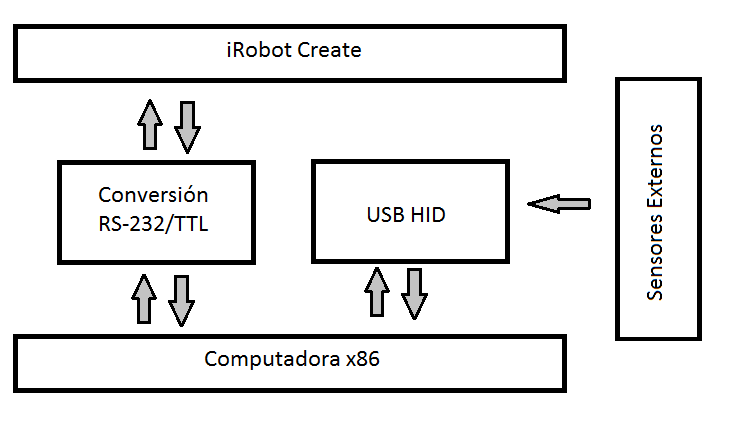
\includegraphics[width=0.8\textwidth]{figures/bloquesHardware.png}
\caption{Diagrama a bloques de la estructura del hardware}
\centering
\label{fig:bloquesHardware}
\end{center}
\end{figure} 
\textbf{iRobotCreate:} la plataforma robótica que se comunica con el resto del sistema mediante el estándar RS-232 a través de un puerto DB-25 con dos terminales dedicadas a ello.\\
\textbf{Conversión RS-232/TTL:} Este módulo funciona como intermediario y se encarga de la conversión de niveles de voltaje RS-232 (hasta +/- 15v) a niveles TTL (hasta +/- 5v) y viceversa. Está construido a partir de un circuito integrado MAX232.\\
\textbf{USB HID:} Es un bloque basado en un microcontrolador PIC18F4550 cuya función es convertir señales tanto analógicas como digitales provenientes de sensores externos y transmitirlas mediante un flujo de bytes a la computadora.\\ 
\textbf{Sensores externos:} La implementación específica de este módulo dependerá de la aplicación y comprende todos aquellos sensores ajenos al robot que expanden sus capacidades para reconocer su entorno. El diseño actual posee 8 terminales para la conexión de sensores digitales (de niveles TTL) y otras 13 para sensores analógicos cuya salida se encuentre entre 0 y 5v. \\
\textbf{Computadora x86:} Es una de las piezas centrales del sistema y se encarga, además de servir como vínculo entre el resto de los bloques, de coordinar y procesar el flujo de información proveniente del robot durante su operación.\\  


\section{Estructura organizacional del software}
A fin de conseguir un diseño flexible, robusto y altamente portátil, dado el gran número de sistemas operativos compatibles con la arquitectura x86 y las diferencias entre ellos, fué necesario crear un diseño modular a base de capas que permitiera la independencia de sistemas operativos, plataformas e incluso lenguajes de programación. El esquema de la figura \ref{fig:capasSoftware} ilustra este diseño.

\begin{figure}
\begin{center}
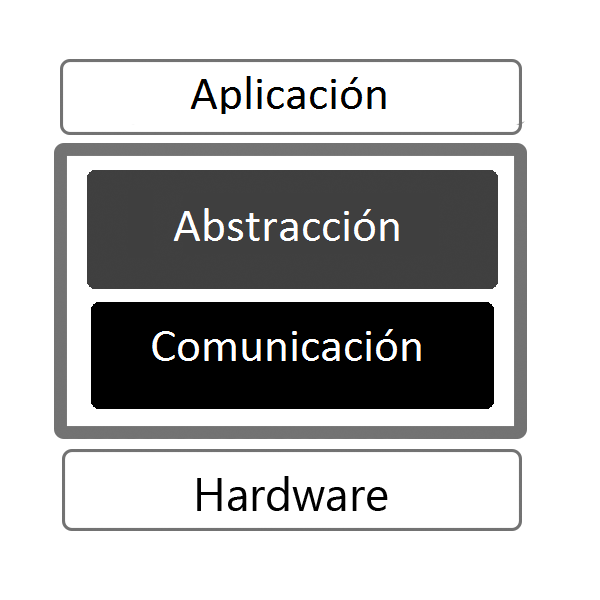
\includegraphics[width=0.8\textwidth]{figures/capas.png}
\caption{Diagrama del modelo en capas del software}
\centering
\label{fig:capasSoftware}
\end{center}
\end{figure}
\subsection{Capa de comunicación}
La comunicación directa con el robot se lleva a cabo en esta capa a través de descriptores de hardware e instrucciones de lectura y escritura operadas directamente sobre ellos. Es aquí donde tiene lugar el verdadero intercambio de datos y debido a su cercanía con el hardware debe ser reimplementada para cada sistema operativo.\\
El siguiente pseudocódigo ejemplifica el tipo de función que se puede encontrar a este nivel:
\begin{lstlisting}
Escribir_a_puerto_Serial(BYTE[] datos)
{
	descriptor_puerto <- abrir(DIRECCION_FISICA_DEL_PUERTO)
	Escribir( descriptor_puerto, datos)
	cerrar(descriptor_puerto)
}

\end{lstlisting}
\subsection{Capa de abstracción}
Su propósito es proveer funciones genéricas, humanamente legibles e independientes de implementación para operaciones de entrada/salida comunes. La abstracción de los componentes de hardware del robot (sensores, LED's, motores, etc) también se lleva a cabo en este nivel. Así, esta capa se convierte en una interfaz que permite la interacción entre las capas superior e inferior. Para su implementación, siempre que el hardware y el lenguaje de programación lo permitan, se puede sacar gran ventaja del uso del paradigma orientado a objetos. Una típica implementación en la capa de abstracción luce como el siguiente pseudocódigo:

\begin{lstlisting}
Clase Robot
{
	ENTERO sensor1
	ENTERO modo
	ENTERO rueda_izquierda

	(...)
	
	Avanzar( ENTERO velocidad)
	{
 		buffer <- [ CODIGO_AVANZAR, velocidad.msb, velocidad.lsb]
		Escribir_a_puerto_Serial(buffer)
	}
}


\end{lstlisting}

\subsection{Capa de aplicación}
Capa a nivel de usuario del programa. Aqui son descritas todas las funcionalidades del robot para una aplicación en específico. Todas las operaciones a bajo nivel deben ser transparentes para el programador. Por ejemplo:\\
\begin{lstlisting}
main( )
{
	[Clase]Robot robot <- new Robot( ) 
	si( no_hay_obstaculos )
		robot.Avanzar( 100 )
}



\end{lstlisting}
\section{Tecnologías a utilizar}
\subsection{Microcontrolador PIC18F4550}
El PIC18F4550 de Microchip es un microcontrolador de bajo costo y consumo. Para este trabajo se utiliza en su encapsulado PDIP de 40 terminales que proporciona cuatro puertos de entrada/salida de entre siete y ocho bits digitales y analógicos, además de un convertidor analógico-digital de 13 canales con resolución de 10 bits. Una de sus características más sobresalientes es el soporte para USB 2.0 de baja (1.5 Mbps) o alta (12Mbps) velocidad, transferencias de control  isocronas, por interrupción y por volumen (\emph{bulk}), con hasta 32 \emph{endpoints} y regulador de voltaje integrado. \cite{pic18datasheet}
\subsection{La arquitectura x86}
La especificación para esta arquitectura fue creada por Intel en 1978 y ha sido el estándar para las computadoras personales durante los últimos 30 años {\cite{smith}} aunque también se encuentra presente en otros dispositivos como plataformas embebidas, SBC y móbiles. Esto proporciona grandes ventajas como la generalizada familiaridad de la mayor parte de los programadores con la arquitectura y la gran disponibilidad de sistemas operativos, software y hardware compatibles. Además, las reducciones de tamaño y consumo eléctrico de las Unidades de Procesamiento Gráfico (GPU) tanto integradas como discretas propician la alineación de la robótica y sistemas inteligentes con la creciente popularidad de la programación gráfica y de propósito general en paralelo \cite{nugteren}, territorio virtualmente inexplorado hasta el momento.

\subsection{c++ 11}
Se trata de un nuevo estándar del lenguaje c++ que introduce algunos cambios al nucleo del lenguaje y adiciones a la biblioteca estándar. Además de mejorar el rendimiento en tiempo de compilación y ejecución, una de sus mayores contribuciones es el soporte para la programación multihilo que se utiliza en este trabajo para el manejo de funciones bloqueantes (por ejemplo la lectura del puerto serial) mediante clases y funciones especializadas en ello.


% %----------------------------------- % %
\chapter{Implementación de hardware}
\section{Alimentación eléctrica}
Uno de los más importantes aspectos a considerar durante el diseño de un circuito como este es la alimentación eléctrica. Dado que la mayoría de los componentes que lo conforman operan al mismo voltaje y a fin de evitar el uso fuentes de energía externas al sistema, se optó por utilizar como fuente primaria la batería propia del robot.\\
El iRobot Create\textsuperscript{\textsuperscript{\textregistered}}, es capaz de alimentar circuitos externos mediante salidas de volaje dedicadas a través de su conector DB-25 (ver \ref{fig:createPinout}) que pueden proporcionar 5v y máximos de 100mA o 1.5A cuando el robot está encendido \cite{irobotm}. Para brindar más flexibilidad al diseño, se han elegido las terminales 9 y 25 como fuente de alimentación que corresponden a las salidas Vpwr y GND de la batería del robot. Los 18v provenientes de la batería son reducidos a 5v mediante un regulador de voltaje positivo L7805CV que admite cargas de hasta 1.5A y cuyo diagrama de conexión se muestra en la figura \ref{fig:L7805}.

\begin{figure}
\begin{center}
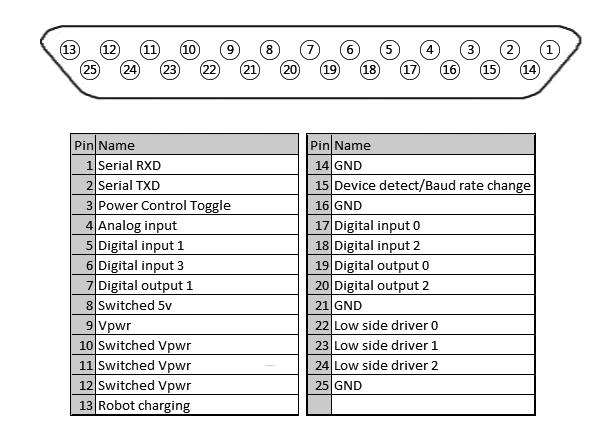
\includegraphics[width=0.8\textwidth]{figures/createPinout.png}
\caption{Diagrama de entradas/salidas del puerto DB-25 en el iRobot Create\textsuperscript{\textsuperscript{\textregistered}}}
\centering
\label{fig:createPinout}
\end{center}
\end{figure} 

\begin{figure}
\begin{center}
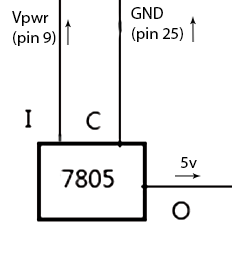
\includegraphics[width=0.8\textwidth]{figures/lm7805.png}
\caption{Regulación de volaje mediante un L7805CV}
\centering
\label{fig:L7805}
\end{center}
\end{figure} 

\section{Circuito para la conexión serial RS-232}
Como se mencionó anteriormente, la comunicación entre la computadora de arquitectura x86 y el iRobot Create\textsuperscript{\textsuperscript{\textregistered}} se lleva a cabo mediante una conexión serial RS-232 pero que debido a limitaciones de hardware  debe ser convertida a niveles TTL antes de ser utilizada. Esto se logra mediante el circuito integrado MAX232 cuyos capacitores externos llevan a cabo las multiplicaciones y divisiones de voltaje necesarias para convertir los hasta +/- 15v  definidos en el estándar a los +/- 5v requeridos por el robot.
En la figura \ref{fig:diagramars232} se muestran los circuitos para la conversión de voltajes y la comunicación serial. El conector  DB-9 hembra se acopla a la computadora x86 y el DB-25 macho se conecta al Create\textsuperscript{\textsuperscript{\textregistered}}.
\begin{figure}
\begin{center}
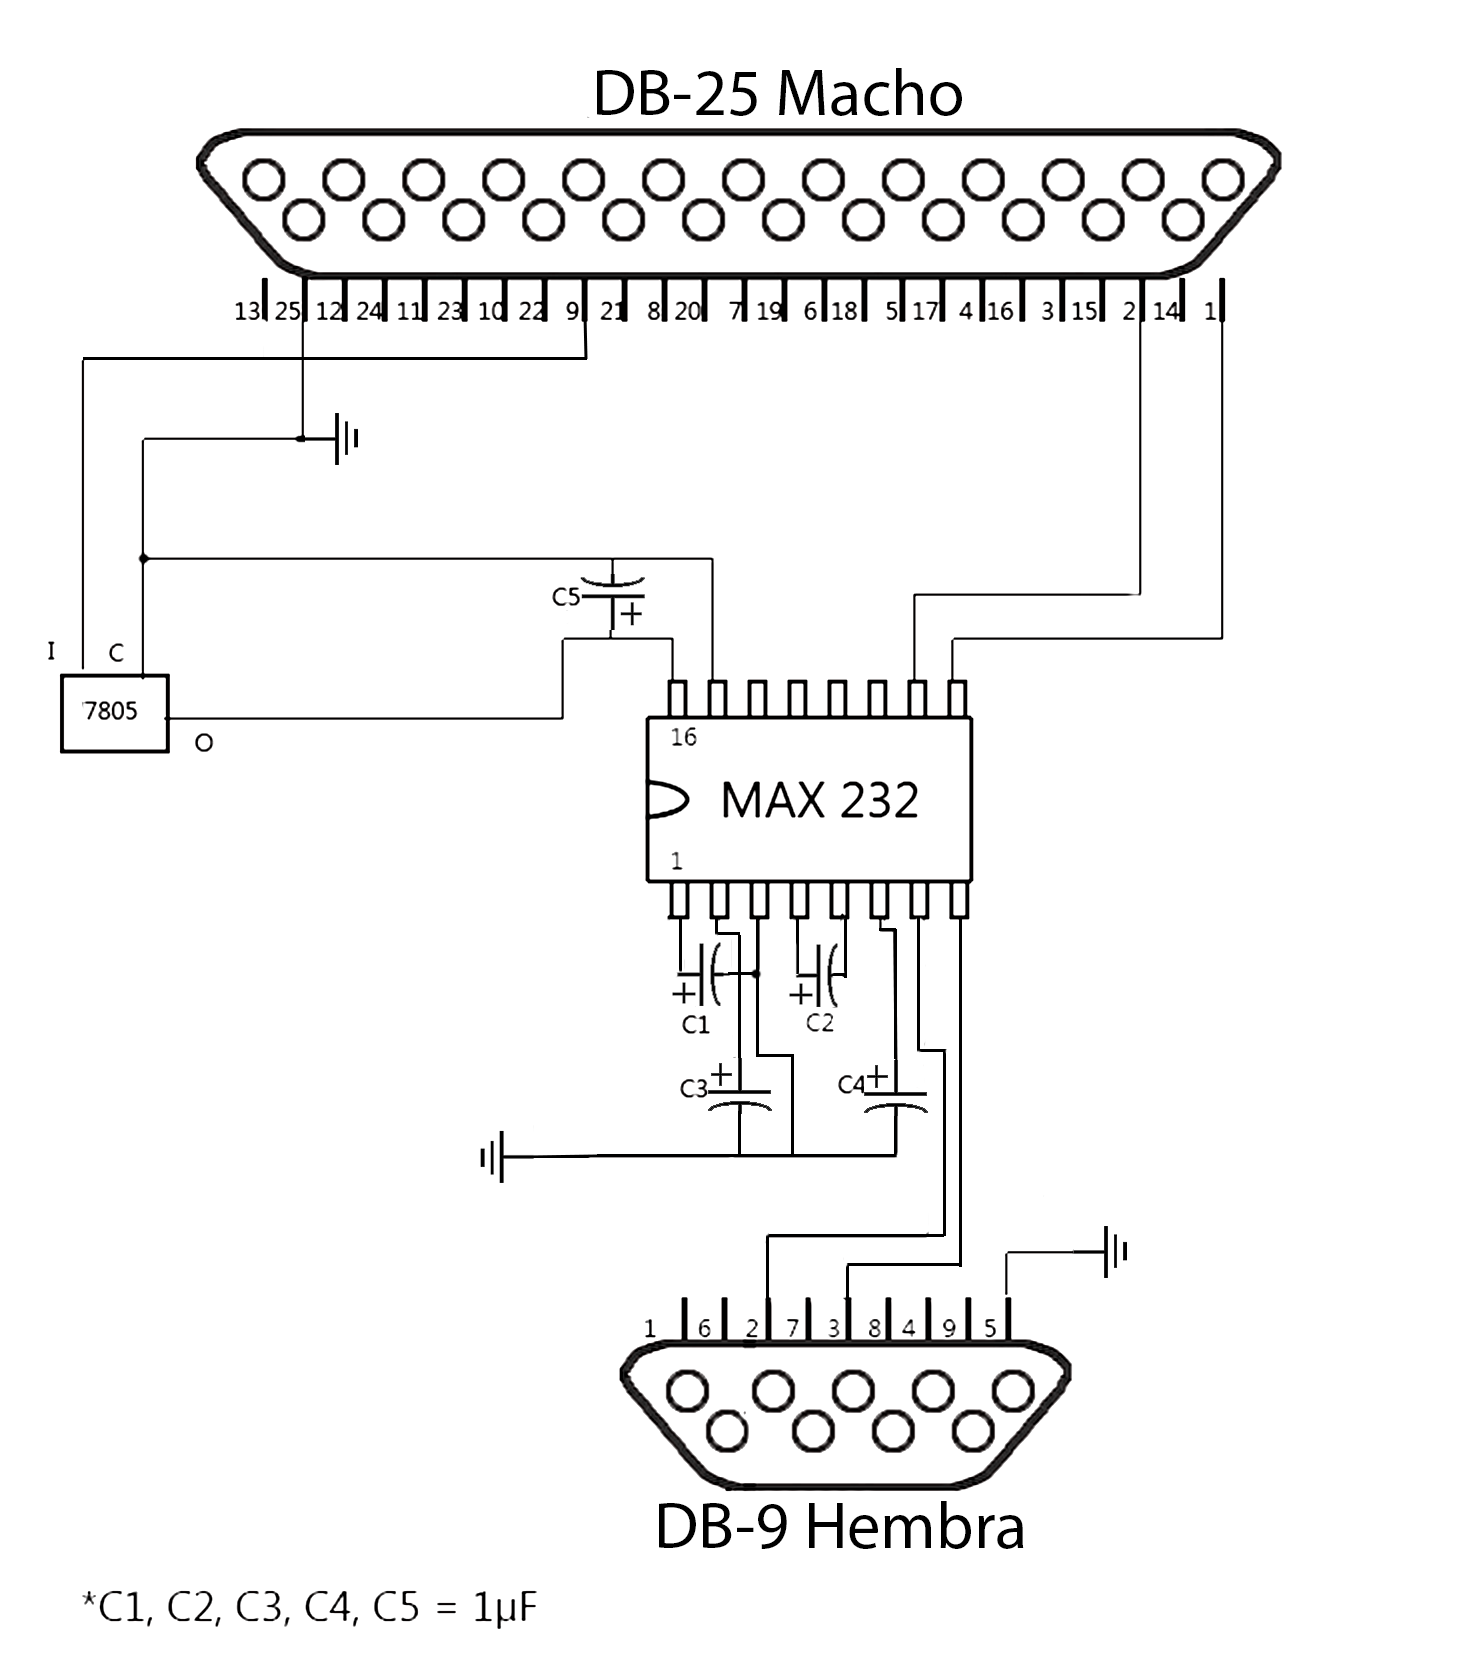
\includegraphics[width=0.8\textwidth]{figures/max232.png}
\caption{Diagrama eléctrico del circuito para la comunicación serial RS-232}
\centering
\label{fig:diagramars232}
\end{center}
\end{figure} 
\section{Circuito para la comunicación USB 2.0}
En la figura \ref{fig:diagramaUSB} se muestra un diagrama esquemático de las conexiones eléctricas necesarias para la comunicación USB. La parte central de este sistema la conforma el microcontrolador PIC18F4550. El resistor R1 se utiliza a manera de \emph{pull-up} para evitar la reinicialización del microcontrolador. Los resitores del R2 al R24, se utilizan como \emph{pull-down} para forzar un nivel lógico bajo cuando los sensores externos no estan conectados. Los resistores R25 y R26 disminuyen la corriente que llega a los diodos LED D1 y D2 utilizados para indicar el estado general del sistema. El oscilador XTAL1 provee el pulso de reloj principal para la ejecución del programa registrado en el microncontrolador y está además conectado a los capacitores Ca y Cb para disminuir el ruido en la señal del mismo. El capacitor Cc es un requisito de hardware establecido por el fabricante \(Microchip\)  para la comunicación USB. Los pines 23 y 24 se conectan a las terminales D- y D+ del conector USB macho respectivamente y es a través de ellas que se transporta el flujo de datos entre el microcontrolador y la computadora x86.
\begin{figure}
\begin{center}
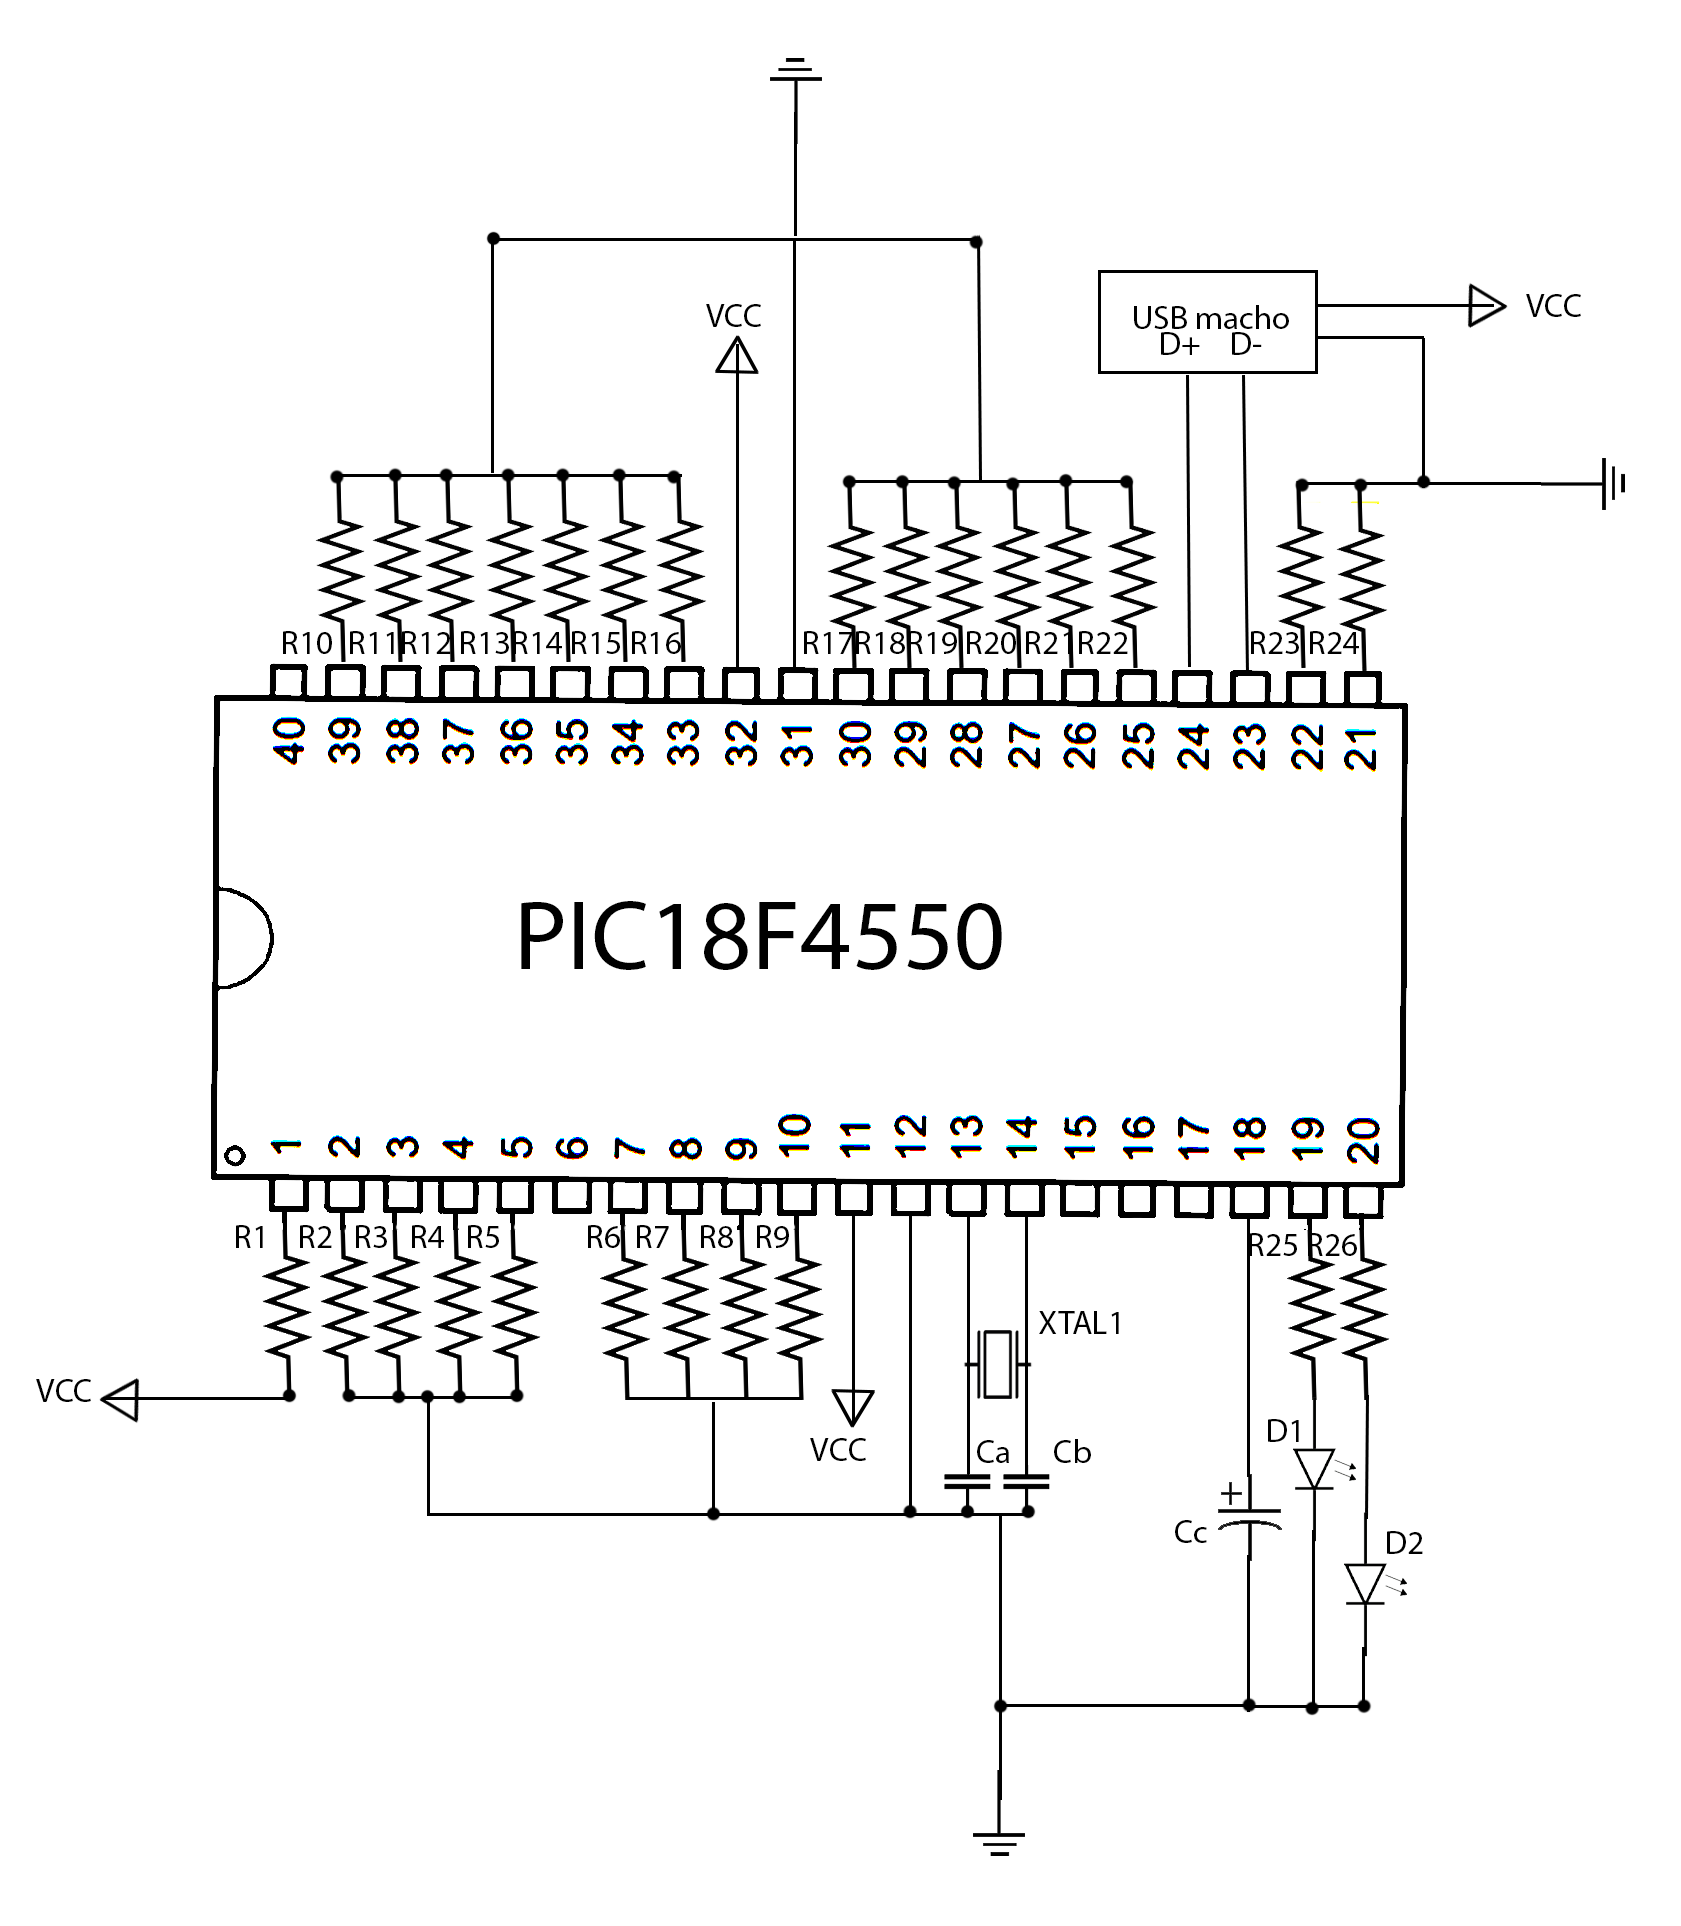
\includegraphics[width=0.8\textwidth]{figures/diagramaUSB.png}
\caption{Diagrama eléctrico del circuito para la comunicación USB}
\centering
\label{fig:diagramaUSB}
\end{center}
\end{figure} 
\chapter{Implementación de Software}
El software de este proyecto se divide en dos grnades partes. Una de ellas es el firmware del microcontrolador, codificado en lenguaje c en el ambiente MPLAB y compilado con c18 de microchip. El otro es el software de la biblioteca UDG\_Create programado en c/c++  y compilado en g++.\\
\section{Firmware del microcontrolador}
Para facilitar la implementación de dispositivos que cumplan con el estandar USB, Microchip, fabricante del microcontrolador PIC18F4550, proporciona el \emph{MCHPFSUSB Firmware Framework}, un conjunto de ejemplos en los que se implementan distintas funcionalidades relativas a este estándar. El firmware para este trabajo está basado en el ejemplo\emph{ USB Device - HID - Simple Custom Demo - C18 - PICDEM FSUSB\ } de dicho framework. Algunas de sus principales características se describen a continuación.\\
\subsection{Configuración del oscilador para la comunicación USB 2.0}
La comunicación USB de velocidad completa en el PIC18F4550 requiere utilizar un pulso de reloj de 48MHz que debe ser tomada del oscilador primario y que en general será alcanzada mediante pre y post escaladores cuyas configuraciones por software dependerán del hardware disponible.\\
La configuración de reloj a utilizar, para un cristal de 4MHZ es:
\begin{lstlisting}
 //Sin pre-escala para entrada de PLL
#pragma config PLLDIV   = 1       
//PLL = 96MHz /2   
#pragma config CPUDIV   = OSC1_PLL2 
//Usar PLL/2 como reloj USB
#pragma config USBDIV   = 2     
//Habilitar oscilador de alta velocidad y PLL    
#pragma config FOSC     = HSPLL_HS  

\end{lstlisting}

De esta forma obtenemos una frecuencia de 4MHz a la entrada del PLL y 48 MHz a la salida del mismo que serán utilizados como reloj para los módulos USB. En el caso particular del PIC18, durante la operación USB, otros periféricos pueden operar a velocidades menores por lo que esto no representará un problema de compatibilidad.\\

      
\subsection{Descriptores USB}
En los sistemas basados en USB, el intercambio de datos se hace a través de \emph{endpoints} mediante mensajes llamados reportes, conformados de manera específica y cuya organización está definida en estructuras llamadas descriptores.\\
Los descriptores comienzan con su propio tamaño en bytes, seguidos de su tipo (necesario para ser interpretado correctamente por el \emph{host}) y después una serie de campos específicos para cada descriptor. Por ejemplo:
\begin{lstlisting}
typedef struct{ BYTE bLength;  // Tamano en bytes
	BYTE bDescriptorType; //tipo
	bcdUSB;  //numero de release
	BYTE bDeviceClass;  //clase de dispositivo
	bDeviceSubClass;    //sub-clase de dispositivo
	BYTE bDeviceProtocol;  //codigo de protocolo
	BYTE bMaxPacketSize0;  //Tamano maximo para EP0
	WORD idVendor;    //ID de fabricante
	WORD idProduct;   //ID de producto
	WORD bcdDevice;   //numero de release
	BYTE iManufacturer;   // indice de descriptor
	BYTE iProduct;       // descriptor de producto
	BYTE iSerialNumber;  //Numero de serie
	BYTE bNumConfigurations;     //numero de configuraciones
}device_descriptor;            
\end{lstlisting}

\textbf{Definición de cadenas}\\
Las cadenas de carácteres a las que tendrá acceso el dispositivo USB deben ser almacenadas como estructuras de datos que incluyen tamaño, tipo de estructura y los datos como tales dentro de una zona de memoria ROM determinada. Las 3 cadenas necesarias son las siguientes:

\begin{lstlisting}
//Descriptor de codigo de lenguaje
ROM struct{BYTE bLength;BYTE bDscType;WORD string[1];}sd000={
sizeof(sd000),USB_DESCRIPTOR_STRING,{0x0409
}};

//Descriptor de cadena de fabricante
ROM struct{BYTE bLength;BYTE bDscType;WORD string[25];}sd001={
sizeof(sd001),USB_DESCRIPTOR_STRING,
{'M','i','c','r','o','c','h','i','p',' ',
'T','e','c','h','n','o','l','o','g','y',' ','I','n','c','.'
}};

//Descriptor de cadena de producto
ROM struct{BYTE bLength;BYTE bDscType;WORD string[20];}sd002={
sizeof(sd002),USB_DESCRIPTOR_STRING,
{'C','r','e','a','t','e',' ','R','o','b','o','t',' ','S','e','n','s','o','r','s'}};

\end{lstlisting}
Estas cadenas son a su vez almacenadas en otra estructura de datos que las agrupa. Las referencias futuras a las cadenas (en los descriptores de dispositivo y de configuración) se hacen en relación a la siguiente definición:
\begin{lstlisting}
//Arreglo de descriptores de cadena
ROM BYTE *ROM USB_SD_Ptr[]=
{
    (ROM BYTE *ROM)&sd000,
    (ROM BYTE *ROM)&sd001,
    (ROM BYTE *ROM)&sd002
};
\end{lstlisting}
\textbf{Descriptor de dispositivo}\\
Los campos identificador de fabricante (0x04D8) e identificador de dispositivo (0x003F) en este descriptor son de especial importancia porque es a través de ellos que iniciaremos la comunicación entre el driver HID del Sistema Operativo y el microcontrolador. 
\begin{lstlisting}

ROM USB_DEVICE_DESCRIPTOR device_dsc=
{
    0x12, //tamano en bytes
    USB_DESCRIPTOR_DEVICE,  //tipo de dispositivo
    0x0200,                 // version USB
    0x00,                   // Codigo de clase
    0x00,                   // codigo de subclase
    0x00,                   //codigo de protocolo
    USB_EP0_BUFF_SIZE,      //Tamano max para EP0 (8)
    0x04D8,                 //ID fabricante 
    0x003F,                 //ID producto 
    0x0002,                 //Release dispositivo
    0x01,                   //cadena de fabricante
    0x02,                   //cadena de producto
    0x00,                   //numero de serie
    0x01                    // posibles configuraciones
};
\end{lstlisting}

\textbf{Descriptor de configuración}\\
Define la única configuración posible para este dispositivo. Se encapsula en una sola estructura de datos toda la información necesaria para la operación USB inlcuyendo el protocolo de comunicación y clase de dispositivo a utilizar (HID), longitud, tipo y formato de los reportes asi como la dirección, longitud y tipo de uso de los endpoints de entrada y salida.
\begin{lstlisting}
ROM BYTE configDescriptor1[]={
   	0x09,  //Tamano de descriptor
    USB_DESCRIPTOR_CONFIGURATION,   // Tipo de descriptor (0x02)
    0x29,0x00,              //Longitud de datos de configuracion
    1,                      //Numero de interfaces
    1,                      //Indice de la configuracion
    0,                      //Indice de la cadena de configuracion
    _DEFAULT | _SELF,               //Atributos,
    50,                     // max consumo de potencia (2X mA)
							
    /*Descriptor de Interfaz */
    0x09,//sizeof(USB_INTF_DSC),   // Tamano
    USB_DESCRIPTOR_INTERFACE,     //Tipo de descriptor (0x04)
    0,                             // Numero de interfaz
    0,                 // Numero de configuracion alternativo
    2,                            // Numero de endpoints
    HID_INTF,                     // Codigo de clase HID (0x03)
    0, // Codigo de subclase
    0, // codigo de protocolo
    0, //Indice de cadena

   /*Descriptor  de Reporte HID*/
    0x09,//sizeof(USB_HID_DSC)+3,    // Tamano de descriptor
    DSC_HID,                        // Tipo de descriptor (0x21)
    0x11,0x01,           // version de especificacion HID (1.11)
    0x00,                // Codigo de pais (0x00 = no soportado)
    HID_NUM_OF_DSC,                // Numero de descriptores (1)
    DSC_RPT,                //Tipo de descriptor (0x22, reporte)
    HID_RPT01_SIZE,0x00, //tamano de descriptor de reporte
    
    /* Descriptor enpoint IN */
    0x07,/*sizeof(USB_EP_DSC)*/
    USB_DESCRIPTOR_ENDPOINT,    //Descriptor de endpoint (0x05)
    HID_EP | _EP_IN,           //Direccion de endpoint (1|0x80)
    _INTERRUPT,                 //Atributos (0x03)
    0x40,0x00,                  //Tamano
    0x01,                       //Intervalo

    /* Descriptor endpoint OUT*/
    0x07,  //tamano de descriptor
    USB_DESCRIPTOR_ENDPOINT,  //Descriptor de endpoint (0x05)
    HID_EP | _EP_OUT,         // Direccion de endpoint (1|0x00)
    _INTERRUPT,               //Atributos (0x03)
    0x40,0x00,                //Tamano
    0x01                     //Intervalo
};
\end{lstlisting}

Todas las configuraciones posibles deben ser almacenadas en un arreglo. Toda referencia a estas configuraciones debe hacerse de acuerdo a la siguiente definción:
\begin{lstlisting}
ROM BYTE *ROM USB_CD_Ptr[]=
{
    (ROM BYTE *ROM)&configDescriptor1
};
\end{lstlisting}
\subsection{Configuración de puertos}
Los cuatro puertos de entrada/salida del PIC18F4550 son configurados mediante los registros \emph{LATX} y \emph{TRISX} donde \emph{X} corresponde al identificador del puerto (A,B,C o D) y es a través de ellos que se lee/escribe su valor y se determina su dirección. Otros registros de control específicos de cada puerto definirán su funcionalidad.\\
Para este trabajo, una parte de los puertos A y B (terminales 2, 3, 4, 5, 7, 8, 9, 10, 33, 34, 35, 36 y 37) se destinan a la conversión de señales analógicas provenientes de sensores externos a datos digitales en cuyo caso se omite la configuración del registro TRISX ya que se incluye en ADCON1.PCFGX. Los dos bits restantes del puerto B (terminales 38 y 39) se utilizan para leer las señales digitales de carga y poder del robot.

\begin{lstlisting}
//B5 (RobotOn) como entrada
TRISBbits.TRISB5=1;
//B6 (RobotCharging) como entrada
TRISBbits.TRISB6=1;

//AN0 - AN12 como entradas analogicas, se omite TRISX
ADCON1bits.PCFG3=0;
ADCON1bits.PCFG2=0;
ADCON1bits.PCFG1=0;
ADCON1bits.PCFG0=0;


\end{lstlisting}

Los bits 0 y 1 del puerto D se conectan a dos diodos LED que se utilizan como indicadores de estado por lo que son configurados como pines digitales de salida. El resto de los bits del puerto D asi como los bits 6 y 7 del C se usan como entradas para sensores digitales.

\begin{lstlisting}
TRISDbits.TRISD0 = 0; //Salida LED
TRISDbits.TRISD1 = 0; //Salida LED
TRISDbits.TRISD2 = 1; //entrada para sensor digital
TRISDbits.TRISD3 = 1; //entrada para sensor digital
TRISDbits.TRISD4 = 1; //entrada para sensor digital
TRISDbits.TRISD5 = 1; //entrada para sensor digital
TRISDbits.TRISD6 = 1; //entrada para sensor digital
TRISDbits.TRISD7 = 1; //entrada para sensor digital
	

TRISCbits.TRISC6 = 1; //entrada para sensor digital
TRISCbits.TRISC7 = 1; //entrada para sensor digital
\end{lstlisting}

\subsection{Lectura de sensores externos}
La lectura de sensores externos se lleva a cabo dentro de un bucle infinito al principio del cual, mediante una operación de lectura bloqueante se esperan reportes del host USB principal. Cuando el identificador de resporte es 0x37 se inicia la lectura de los sensores externos los cuales son convertidos a información digital y empaquetados como un arreglo de bytes en el que la primer posición es un eco del identificador de reporte recibido, posteriormente se almacenan 13 pares de bytes correspondientes a la conversión de los sensores analógicos (byte mas significativo en la posición de memoria más baja) y por último 8 bits de sensores digitales. Este arreglo se envía como respuesta al host USB.\\
La lectura de los sensores analógicos requiere un proceso de conversión digital. Los registros asociados a la configuración del convertidor analógico-digital del microcontrolador son ADRESH y ADRESL que almacenan el resultado de la conversión y los registros de control ADCON0, ADCON1 y ADCON2.\\
Para la configuración inicial del registro ADCON0 solamente fijaremos en alto el bit 0, correspondiente a la habilitación/deshabilitación del módulo de conversión. El resto de los bits (selección de canal e inicio de conversión ) se establecerán en el momento de iniciar una conversión nueva.\\
Los bits 4 y 5 del registro ADCON1 (VCFG1:VCFG0) indican el voltaje analógico de referencia para la conversión, los cuales serán 0 para que se utilicen los voltajes VSS y VDD. El resto de los bits de este registro (PCFG3:PCFG0) se fija a 0 durante la configuración de puertos.\\
El bit 7 del registro ADCON2 es un bit de justificación, esto es, especifica el desplazamiento del resultado de 13 bits dentro del registro de 16 bits que forman en conjunto ADRESH y ADRESL de manera que, de ser necesario se desprecien lo bits menos significativos o viceversa. Debido a que los bytes alto y bajo del resultado de la conversión se tratarán por separado, se eligió la justificación a la derecha, es decir, el bit ADFM en nivel alto. Los bits 3, 4 y 5 corresponden al tiempo de adquisición mínimo para la conversión, el tiempo que se debe esperar para que el capacitor CHOLD se carge hasta el voltaje de entrada. Ya que desconocemos a priori la impedancia total que tendrán los sensores, asignamos el valor más alto posible (20$T_{AD}$) a fin de no perder precisión en las mediciones. Por último, los bits 0, 1 y 2 nos permiten elegir la fuente de reloj para el módulo, que  será $F_{OSC}/4$.


\begin{lstlisting}
ADCON0=0x01;
ADCON1=0x00;
ADCON2=0x3C;
ADCON2bits.ADFM = 1;
\end{lstlisting}

Para llevar a cabo la conversión, con la ayuda de un contador controlado por un ciclo for, modificamos los bits de selección de canal CHS3:CHS0 en el registro ADCON0 y fijamos el bit GO a 1. Posteriormente debemos esperar al cambio de estado del bit GO indicando que la conversión ha finalizado. Entonces almacenamos el contenido de ADRESH y ADRESL en posiciones contiguas del buffer de salida y continuamos con la siguiente conversión.\\

\begin{lstlisting}
unsigned char i;
ToSendDataBuffer[0] = 0x37;	//Eco
for(i=0;i<13;i++)
	{						
	 ADCON0=(i<<2)+1; //cambio de canal					
	 ADCON0bits.GO = 1;  //inicio de conversion     
	 while(ADCON0bits.GO); //esperar fin de conversion
	 ToSendDataBuffer[2*i+1] = ADRESL;  	//LSB de resultado
	 ToSendDataBuffer[2*i+2] = ADRESH;  	//MSB de resultado
	}    
\end{lstlisting}

Debido a que los bits asignados a la lectura de sensores digitales no son contiguos y se encuentran de hecho distribuidos en más de un puerto, estos deben ser analizados bit por bit y, en caso de existir un nivel alto de voltaje en ellos, asignar el valor correspondiente al dicho bit mediante un operador OR a una variable originalmente inicializada en 0.

\begin{lstlisting}
ToSendDataBuffer[27] = 0x00;
						
if(PORTDbits.RD7==1)
{
	ToSendDataBuffer[27]|=0x80;
}
if(PORTDbits.RD6==1)
{
	ToSendDataBuffer[27]|=0x40;
}
if(PORTDbits.RD5==1)
{
	ToSendDataBuffer[27]|=0x20;
}
if(PORTDbits.RD4==1)
{
	ToSendDataBuffer[27]|=0x10;
}
if(PORTCbits.RC7==1)
{
	ToSendDataBuffer[27]|=0x08;
}
if(PORTCbits.RC6==1)
{
	ToSendDataBuffer[27]|=0x04;
}
if(PORTDbits.RD3==1)
{
	ToSendDataBuffer[27]|=0x02;
}
if(PORTDbits.RD2==1)
{
	ToSendDataBuffer[27]|=0x01;
}
\end{lstlisting}
\section{Interacción con el driver HID}
Como se menciono anteriormente, una de las ventajas de desarrollar dispositivos USB de la clase HID, es el hecho de que la mayoría de los sistemas operativos modernos poseen por defecto un driver compatible. Sin embargo, es necesaria la creación de un software de nivel intermedio que permita la interacción entre el programa de usuario y el driver a nivel de kernel. En Ubuntu y la mayoría de los sistemas basados en Linux esto es posible gracias a la API definida en el archivo de encabezado linux/hiddev.h.

\section{Comunicación mediante el estándar RS-232}
Enviar instrucciones al iRobot Create\textsuperscript{\textsuperscript{\textregistered}} implica escribir códigos de operación a través del puerto serial de la computadora x86 siguiendo la sintaxis establecida en la \emph{Create Open Interface}. La biblioteca UDG\_Create proporciona una interfaz de alto nivel que permite a los desarrolladores escribir código en c++ sin preocuparse por  especificaciones eléctricas o intercambio de datos a bajo nivel. Las siguientes secciones proporcionan un panorama general del intercambio de instrucciones y datos entre el Create\textsuperscript{\textsuperscript{\textregistered}} y la computadora.\\
\section{Comunicación serial en Linux}
Las operaciones de lectura y escrtura del puerto serial, por estar fuertemente ligadas al hardware, son dependientes del sistema operativo. Para la implementación de la biblioteca UDG\_Create, basada en la distribución de linux Ubuntu 12.10, se utiliza la API de UNIX definida en el archivo de encabezado termios.h y los tipos de datos declarados en fcntl.h.\\
Tal como es costumbre en sistemas basados en UNIX, estas operacions se ejecutan mediante las instrucciones read() y write() operadas sobre un archivo de enlace simbólico asociado con el respectivo puerto serial, al que se hace referencia mediante una variable entera que funge como descriptor de archivo. La apertura de este descriptor se efectua mediante:
\begin{lstlisting}
int portDescriptor = open(portName, O_RDWR | O_NOCTTY | O_NDELAY);
\end{lstlisting}

donde O\_RDWR, O\_NOCTTY y O\_NDELAY indican la apertura en modo de lectura y escritura, la no asignación del puerto como terminal de control del proceso y el establecimiento de operaciones no bloqueantes respectivamente. La variable portName es una cadena de carácteres que contiene el nombre del enlace simbólico a utilizar, el cual debe ser proporiconado por el usuario.\\
La biblioteca UDG\_Create proporciona además un modo de apertura automático en el que se itera a través de los primeros 50 enlaces simbólicos con prefijo ttyS (ttyS1, ttyS1, ttyS2, etc) comunmente asociados al puerto RS-232 y los primeros 10 enlaces con prefijo ttyUSB utilizados para la comunicación serial mediante adapatadores USB en aquellos sistemas que carecen de un conector DB-9 macho.\\
El resto de las configuraciones se efectuan utilizando la estructura llamada termios como se muestra en la siguiente porción de código:
\begin{lstlisting}
struct termios configuration;
//ignorar break, deshabilitar traducciones entre CR y NL,
deshabilitar bits de paridad, deshabilitar control de flujo
configuration.c_iflag &= ~(IGNBRK | BRKINT | ICRNL |
                    INLCR | PARMRK | INPCK | ISTRIP | IXON);
configuration.c_oflag=0;
//deshabilitar echo, modo canonico, procesamiento 
//de entradas personalizado
configuration.c_lflag &= ~(ECHO | ECHONL | ICANON | IEXTEN | ISIG);
//fijar mascara de caracteres de 8 bits
configuration.c_cflag &= ~(CSIZE | PARENB);
configuration.c_cflag |= CS8;
//read() se considera terminado despues de 1 caracter
configuration.c_cc[VMIN]  = 1;
//read() se considera terminado despues de 0 decimas de segundo
configuration.c_cc[VTIME] = 0;
//fijar  baudrate de 57600
cfsetispeed(&configuration, B57600) < 0 ||
 cfsetospeed(&configuration, B57600);
 //aplicar cambios de manera inmediata
tcsetattr(portDescriptor, TCSANOW, &configuration);
\end{lstlisting}

Una vez realizadas estas configuraciones, leer y escribir al puerto serial se logra mediante:
\begin{lstlisting}
write(portDescriptor,buffer,numberOfBytes);
read(portDescriptor,buffer,numberOfBytes);
\end{lstlisting}

\subsection{Formato básico de instrucción}
Como se mencionó anteriormente, para la Create Open Interface, una instrucción consiste en un flujo de datos que inicia con un código de operación correspondiente a una instrucción y es seguido, de requerirlo, por un número determinado de bytes de datos, que deben ser escritos a través de un puerto serial RS-232.

\begin{lstlisting}
CodigoOp [DatosByte1	DatosByte2 DatosByte3... DatosByteN]
\end{lstlisting}
tal como se ejemplifica en el siguiente pseudocódigo para una instrucción genérica

\begin{lstlisting}
TIPO_RETORNO Instruccion(BYTE datos1, DWORD datos2 )
{
	BYTE buffer[3]  <-  [ CODIGO_OP, datos1, datos2.msb, datos2.lsb ]
	Escribir_Serial( PUERTO, buffer, size( buffer) )
}

\end{lstlisting}
Cabe resaltar que independientemente del tipo de datos de los parámetros que pudieran recibirse como argumentos a alto nivel, estos siempre serán divididos y enviados como bytes independientes al robot junto con el resto de los datos y el código de operación.\\
Un claro ejemplo de ello es la función  waitDistance() que indica al robot que debe esperar hasta que cierta distancia, definida por la variable entera \emph{distance}, sea recorrida antes de recibir otra instrucción. Su implementación en lenguaje c++ es la siguiente:\\
\begin{lstlisting}
void Robot::waitDistance(int distance)
{
	if(modo == FULL || modo == SAFE || modo == PASSIVE)
	{
		int16 data1 = toInt16(distance);
		unsigned char ins[3]{0x9C,data1.H,data1.L};
		WriteToSerial(descriptorPuerto,ins,3);
	}
	else
		error(MODO_INVALIDO_INSTRUCCION,(char*)"Funcion WAITDISTANCE");
}

\end{lstlisting}
Podemos apreciar como el código de operación correspondiente a la operación Wait Distance de la Create Open Interface, es enviado al puerto serial al principio del buffer de escritura seguida por los dos bytes que en conjunto conforman un entero de 16 bits representando la distancia a esperar.\\
\subsection{Instrucciones de lectura}
Algunas instrucciones (por ejemplo, las consultas de los sensores integrados) requieren que la computadora, además de enviar la instrucción correspondiente, espere una respuesta por parte del robot, la cual debe ser recibida e interpretada adecuadamente. El pseudocódigo para una típica instrucción de lectura es:\\
\begin{lstlisting}
TIPO_RETORNO instruccion_lectura( REF INTEGER sensor )
{
	BYTE[2] instruccion <- {CODIGO_OP, datos}
	Escribir_Serial(PUERTO, instruccion,2)
	BYTE datos[N]
	Leer_Serial(PUERTO, datos, N)
	Ajustar_Orden_bytes( datos, N, sensor, SIGNO  )
}

\end{lstlisting}
Puede observarse como la respuesta del robot debe ser leida, almacenada en un bufer intermedio y despues ajustada a las convenciones de ordenamoento de bytes y tipos de datos de la arquitectura x86.	La función encargada de ello (de la cual se habla a detalle en \ref{sec:endianess} ) es Ajustar\_Orden\_bytes().\\
Para ejemplificar este tipo de instrucción el siguiente segmento de código muestra el procedimiento para la lectura de paquetes de los sensores integrados del Create\textsuperscript{\textregistered}. La implementación final en c++, para facilitar la reutilización de código, está subdividida en 3 funciones:\\
\begin{lstlisting}
int Create::sensors(unsigned char idPacket)
{
	if(idPacket>=0 && idPacket<=42)
	{
		unsigned char ins[2]{0x8E,idPacket};
		WriteToSerial(descriptorPuerto,ins,2);
		int sizePacket = getSizePacket(idPacket);
		return actualizaSensor(idPacket,sizePacket);
	}
	else
		error(FUERA_RANGO,(char*)"Funcion SENSORS");
}

int Create::actualizaSensor(unsigned char idPaquete, int sizeInstruccion)
{	
	unsigned char ins2[sizeInstruccion];
	usleep(120000);
	ReadFromSerial(descriptorPuerto,ins2,sizeInstruccion);
	int ret = -65536;
	int offset=0;
	switch(idPaquete)
	{
		//(...)
		case 8:
			ret = readWall(ins2+offset);
			if(idPaquete < 7)
			{
				offset+= getSizePacket(8);
			}
			if(idPaquete == 8)
				break;
		//(...)
	}
	return ret;
}

int Create::readWall(unsigned char *ins2)
{
	wall = ins2[0];
	int retValue;
	return toLittleEndian(ins2,1,&retValue,UNSIGNED);
}

\end{lstlisting}
La función Create::sensors() se encarga de escribir el código de operacion correspondiente  a la lectura de paquetes y el identificador del sensor a leer. Esta a su vez llama a la función actualizaSensor(), la cual recibe como parametros el ID del paquete de sensores (puede ser más de uno) y el numero de bytes que se espera recibir como respuesta. En esta función se recibe un arreglo de bytes proveniente del robot mediante ReadFromSerial() que representa el valor del sensor solicitado. Por último este arreglo de bytes se opera mediante una función específica de cada sensor (en el ejemplo readWall()) en la que se convierten a tipos de datos nativos de c++ y se realizan los ajustes de orden de bytes, signo y tamaño de datos mediante toLittleEndian().\\

\subsection{Instrucciones de streaming}
Para mejorar el desempeño de ambientes con capacidades limitadas de procesamiento en tiempo real (por ejemplo, aquellos basados en redes inalámbricas) el Create\textsuperscript{\textregistered} es capaz de enviar paquetes con datos provenientes de sus sensores cada 15 milisegundos. El manejo correcto de esta información supone ciertas dificultades que pueden ser abordadas siguiendo tres pasos fundamentales. El primero de ellos es cambiar el estado de la bandera lógica encargada de controlar el streaming de los datos. Esta operación es propia del robot Create\textsuperscript{\textregistered} y se describe en la siguiente función.\\
\begin{lstlisting}
void Create::pauseResumeStream(bool streamState)
{
	
	if(mode == PASSIVE || mode == SAFE || mode == FULL)
	{
		unsigned char ins[2] = {0x96,streamState};
		WriteToSerial(portDescriptor,ins,2);
		streamingState = streamState;
	}
	else
		error(INVALID_INSTRUCTION_MODE,(char*)"Function PAUSERESUMESTREAM");
}

\end{lstlisting}

De acuerdo a las especificaciones de la Create Open Interface, el contenido del flujo de bytes que se recibe como respuesta dependerá de la información solicitada por el usuario, por ello deberá ser cuidadosamente manejada e interpretada. La inicialización del flujo y el nuevo hilo puede hacerse como sigue:


\begin{lstlisting}
void Create::stream(unsigned char* destinationBuffer,void* thread,int n,...)
{
	std::thread *t =(std::thread*)t;
	va_list args;
	va_start(args,n);
	int bytesToRead=3+n;
	//Probar funcion 4/7
	if(n>=0 && n<=43)
	{
	if(mode==PASSIVE || mode == SAFE || mode == FULL)
	{
		unsigned char* ins = new unsigned char[n+2];
		ins[0] = 0x94;
		ins[1] =n;
		
		for(int i = 2;i<n+2;i++)
		{
			ins[i] = (unsigned char)va_arg(args,int);
			bytesToRead+=getSizePacket(ins[i]);
		}
		WriteToSerial(portDescriptor,ins,n+2);
		streamingState = true;
		//Read packets
		 sleep(1);
		  *t= std::thread(ThreadedReadStream,portDescriptor,this,destinationBuffer,bytesToRead);
				//t.join();
	}
	else
		error(INVALID_INSTRUCTION_MODE,(char*)"Function STREAM");
	}
	else
	{
	error(OUT_OF_RANGE,(char*)"Function STREAM");
	}
}

\end{lstlisting}

Ya que en general se recomienda que las operaciones de lectura a puerto serial sean bloqueantes, lo mejor es manejar el flujo de bytes en un hilo de ejecución separado sacando ventaja de las capacidades multi-hilo en los lenguajes de programación, procesadores y sistemas operativos modernos. La interpretación de los datos recibidos debe hacerse en el cuerpo del nuevo hilo:

\begin{lstlisting}
void ThreadedReadStream(int portDescriptor,Create* r,unsigned char*buffer,int numberOfBytes)
{
	while(r->getStreamingState())
	{
		usleep(15000);
		ReadFromSerial(portDescriptor,buffer,numberOfBytes);
	}
}


\end{lstlisting}

\subsection{Ordenamiento de bytes y tipos de datos}
\begin{figure}
\begin{center}
\includegraphics[width=0.8\textwidth]{figures/endianess.png}
\caption{Importancia del correcto manejo de signos y orden de bytes. El ejemplo I) muestra algunas de las posibles interpretaciones para un entero de 16 bits sin signo, solo el inciso c) es correcto. En el ejemplo II) se muestran posibles interpretaciones para un entero negativo, solo el inciso d) es correcto}
\centering
\label{fig:endianess}
\end{center}
\end{figure} 
Una de las mayores dificultades que surgen al intentar controlar este robot mediante una computadora x86 es lidiar con las diferencias entre las maneras de representar los datos como se ilustra en la figura \ref{fig:endianess}. El iRobot Create\textsuperscript{\textregistered} opera usando enteros con y sin signo de 8 y 16 bits recibidos uno a uno en orden \emph{Big Endian}, esto es, con el byte más significativo primero. Por otro lado, la arquitectura x86 utiliza \emph{Little Endian}, es decir que los bytes menos significativos se encuentran en las posiciones de memoria más bajas, con tamaños de datos variables dependiendo del lenguaje de programación, capacidades de hardware y compilador utilizado. De ahi la necesidad de utilizar una función que permita hacer ajustes en las representaciones en memoria de los datos de manera transparente al programador y sin perder portabilidad. Para ello se propone la siguiente función:\label{sec:endianess}


\begin{lstlisting}
int Create::toLittleEndian( unsigned char* source,int nbytes,int* destination,boolSigned sign)
{
	char* tmp;	

	if(sign == UNSIGNED)
	{
	*destination =0;
	
	}
	else
	{
		if(source[0]&0x80) //if it is negative (2's complement)
		{
			*destination =-1;//0xFFFFFFF... only 1's
		}
		else
		{
			*destination = 0;
		}
	}
	
	tmp = (char*) destination;
	for(int i =nbytes -1; i>=0;i--)
	{
		*(tmp+((nbytes-1) - i)) = source[i];
		
	}	


return *destination;

}
\end{lstlisting}
En el código anterior, la variable \emph{source} es un apuntador al arreglo de bytes que contiene la información proveniente del robot, \emph{nbytes} el número de bytes que deben ser considerados como parte del valor, \emph{destination} es un apuntador a la variable entera donde será almacenado de manera definitiva el resultado y \emph{sign} una variable lógica que nos inidca si \emph{source} debe ser considerado una cifra con o sin signo.\\
El primer paso es establecer el valor inicial de la variable \emph{destination} que dependerá del signo esperado del resultado. En caso de tratarse de un número sin signo, el valor de \emph{destination} se inicializa a 0. Si es un número con signo debe verificarse el bit mas significativo del byte más significativo en el arreglo \emph{source} que representa el bit de signo en ambas arquitecturas, mediante la operación \emph{source[0]} $\&$ 0x80. Cuando este bit es 0, significa que el número es positivo y el valor de \emph{destination} debe inicializarse a 0. En caso contrario, cuando el número es negativo, dado que ambas arquitecturas utilizan complemento a 2 para la representación de números negativos, el valor de \emph{destination} se iniciliza a -1, de tal manera que todos sus bits sean 1 independientemente del tamaño en bytes asignado a las variables enteras por el compilador/sistema operativo.\\
El siguiente paso es asignar un apuntador a un tipo de dato de un byte de longitud (unsigned char) a la misma dirección de memoria que \emph{destination}. Por último, con la ayuda de un ciclo for se invierte el orden de los bytes en \emph{source} y se almacenan en \emph{destination}.\\
% %----------------------------------- % %
\chapter{Pruebas y Análisis de resultados}
A fin de medir las capacidades y limitaciones de la biblioteca UDG\_Create, se diseñó un experimento para compararlo directamente contra el Qbot de Quanser.\\
El programa creado para dicha prueba utiliza los sensores en el parachoques del Create\textsuperscript{\textregistered} para detectar objetos en su camino y esquivarlos. La ejecución inicia con el robot avanzando en linea recta hacia el frente hasta que un objeto sea detectado, si el parachoques registra un impacto por el lado izquierdo, girará aproximadamente 38° hacia la derecha. De manera similar, cuando el impacto ocurre por el lado derecho, el giro se efectuará hacia el lado izquierdo. En el caso de un choque frontal, la dirección del giro se determina de forma aleatoria.\\
\begin{figure}
\begin{center}
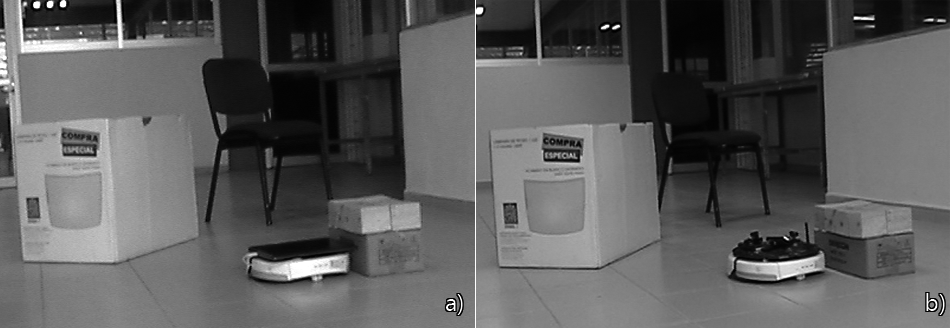
\includegraphics[width=0.8\textwidth]{figures/benchmark.png}
\caption{Comparación entre distintos modelos de progrmación. a) iRobot Create\textsuperscript{\textregistered} y UDG\_Create. b) Quanser Qbot y Simulink}
\centering
\label{fig:benchmark}
\end{center}
\end{figure} 

Ambos robots fueron colocados en un recorrido con obstáculos con las mismas posiciones de inicio de manera que nos permitiera obtener una evaluación cualitativa de su comportamiento bajo las mismas condiciones de operación (ver figura \ref{fig:benchmark}). El Qbot fué programado utilizando simulink y sus respectivos bloques de control  de Quanser, mientras que el software del Create\textsuperscript{\textregistered} fue codificado en c++ utilizando las instrucciones de la biblioteca UDG\_Create (ver \ref{fig:createWorkspace}).\\

\begin{figure}
\begin{center}
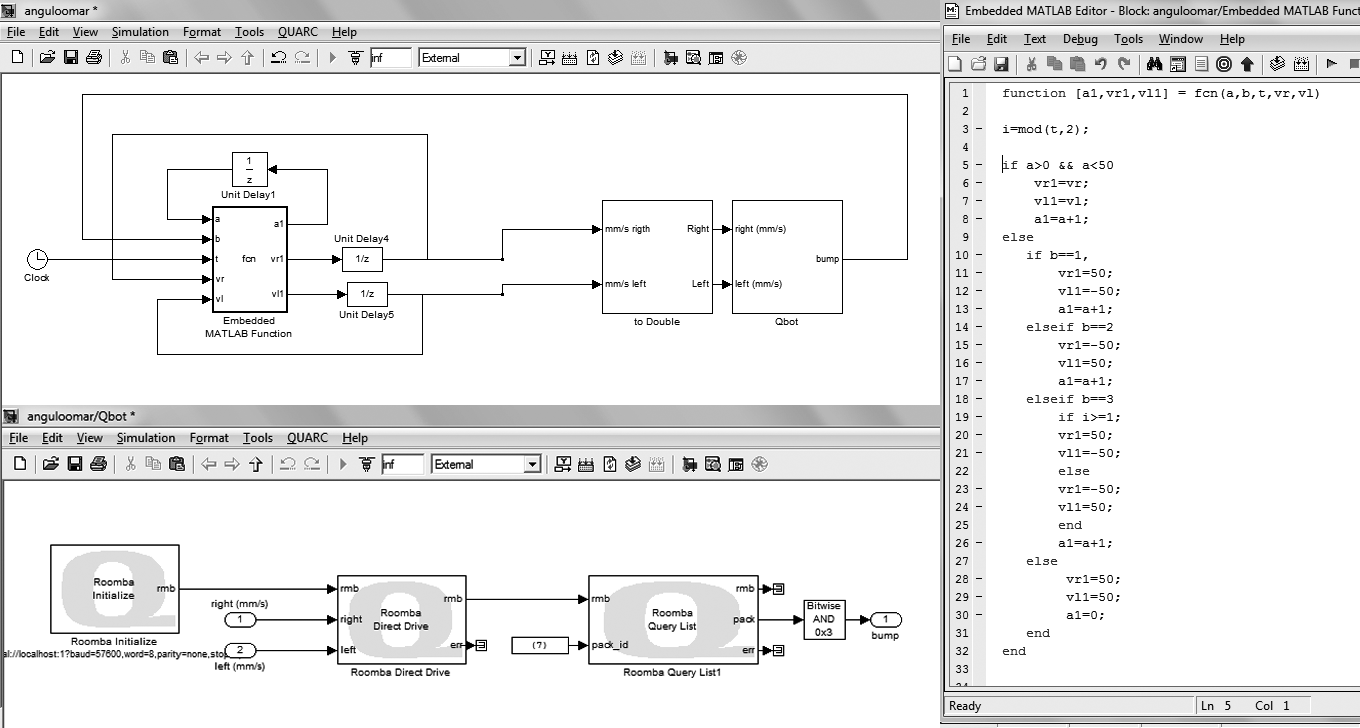
\includegraphics[width=0.8\textwidth]{figures/qbotworkspace.png}
\caption{Ambiente de programación y ejecución del Qbot con Simulink}
\centering
\label{fig:qbotWorkspace}
\end{center}
\end{figure} 

\begin{figure}
\begin{center}
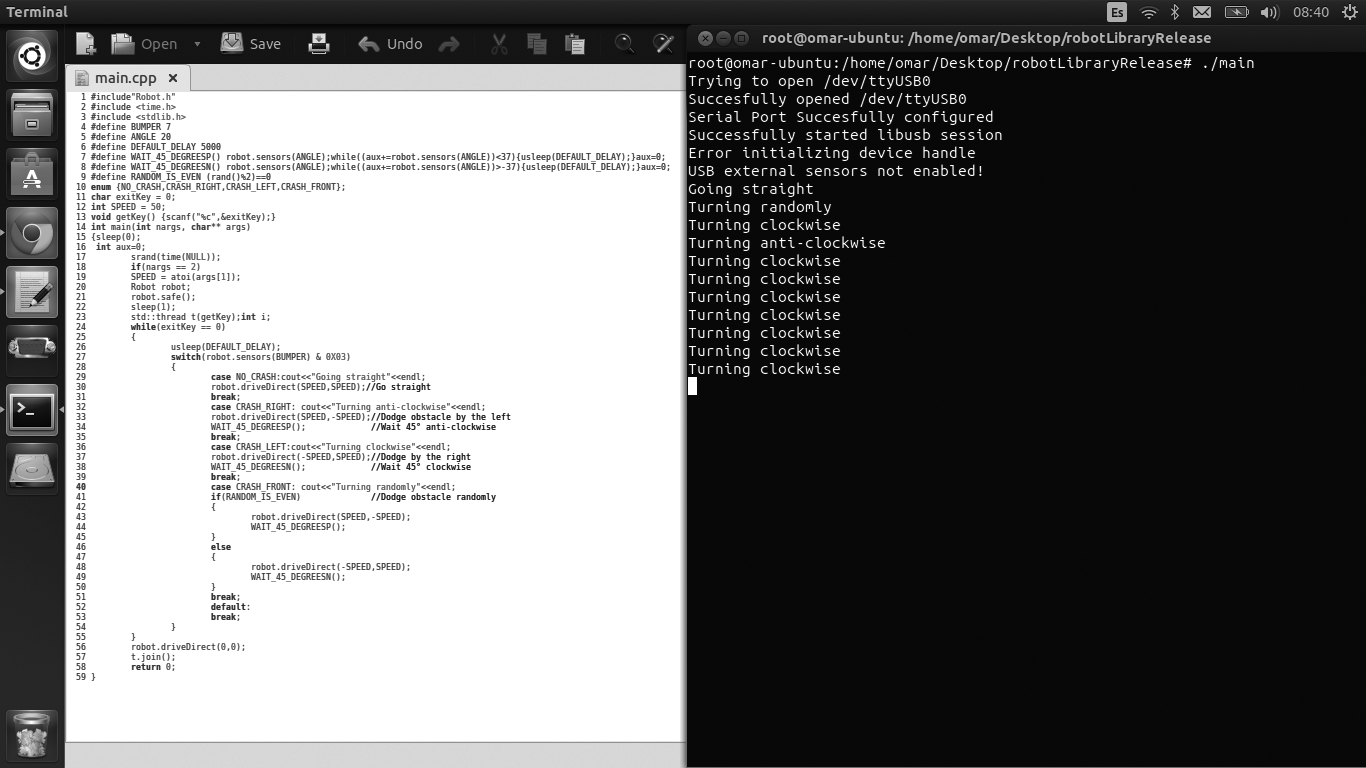
\includegraphics[width=0.8\textwidth]{figures/createWorkspace.png}
\caption{Ambiente de programación y ejecución para el Create\textsuperscript{\textregistered} con UDG\_Create}
\centering
\label{fig:createWorkspace}
\end{center}
\end{figure} 

El comportamiento de ambos robots durante la prueba fue prácticamente idéntico, sin embargo, algunas diferencias significativas tanto cualitativas como cuantitativas (que se resumen en \ref{fig:tabla} ) fueron observadas. En el caso del Qbot, para esta aplicación debido a la complejidad de los protocolos de comunicación inalámbricos y el manejo de sistemas en tiempo real por parte de simulink, una gran cantidad de archivos deben ser generados y copiados a la tarjeta Gumstix integrada del robot para ser compilados en ella. Este proceso inclyendo la compilación tomó un promedio de 65 segundos (porgramas más complejos desarrolados en el laboratorio toman hasta 30 minutos), es decir, 6500\% más lento que la implementación en c++.\\
En cuanto al desempeño, una de las principales ventajas de utilizar lenguajes compilados como c++ en lugar de interpretados como matlab/simulink, es su potencial para ejecutarse hasta 500 veces más rápido (comparado con código de matlab/simulink puro)\cite{andrews}. Esta disimilitud crece aun más cuando, a diferencia del Qbot, se proporciona un enlace cableado entre el robot y la PC. Además, al utilizar software libre para el desarrollo, se evita la compra de las licencias de Matlab/Simulink y QuaRC que pueden llegar a ser muy costosas. Por último, los tiempos de desarrollo y depuración se pueden reducir drásticamente gracias a la familiaridad generalizada de los alumnos con la arquitectura y metodologías de programación y el uso de una biblioteca amigable con el usuario con una curva de aprendizaje no muy pronunciada.\\


\begin{figure}
\begin{center}
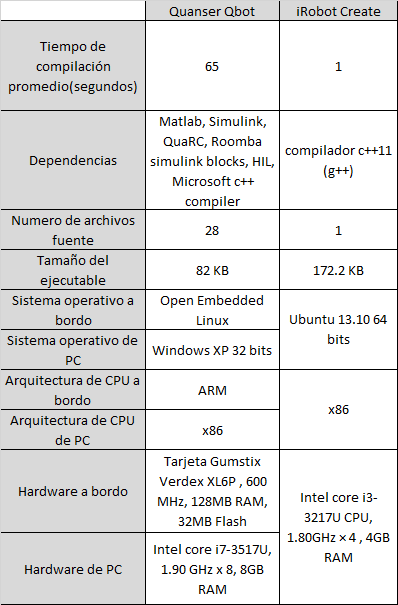
\includegraphics[width=0.8\textwidth]{figures/tabla.png}
\caption{Comparación de configuración entre los robots Qbot y Create\textsuperscript{\textregistered}}
\centering
\label{fig:tabla}
\end{center}
\end{figure} 


% %----------------------------------- % %
\chapter{Manual de Usuario}
\section{La placa fenólica}
Las figuras \ref{fig:pcbSchematics} y \ref{fig:pcb} muestran respectivamente una visión esquemática y física de la placa fenólica para la conexión del robot y los sensores externos con la PC.\\
Posee 13 terminales para sensores analógicos con salidas de 0 a 5v, 8 bits para sensores digitales, un conector DB-9 para comunicación serial con la PC mediante el estándar RS-232, un conector USB 2.0 para la lectura de los sensores externos desde la PC y un conector DB-25 para el intercambio de información con el Create\textsuperscript{\textregistered} desde el conector de su bahía de carga.\\
Para utilizar la biblioteca UDG\_Create, la conexión USB es opcional. Cuando no se requiera el uso de sensores externos es posible sustituir la placa fenólica por el cable serial propio del Create\textsuperscript{\textregistered} o cualquier otro circuito de conversión TTL/RS-232.\\
\begin{figure}[h]
\begin{center}
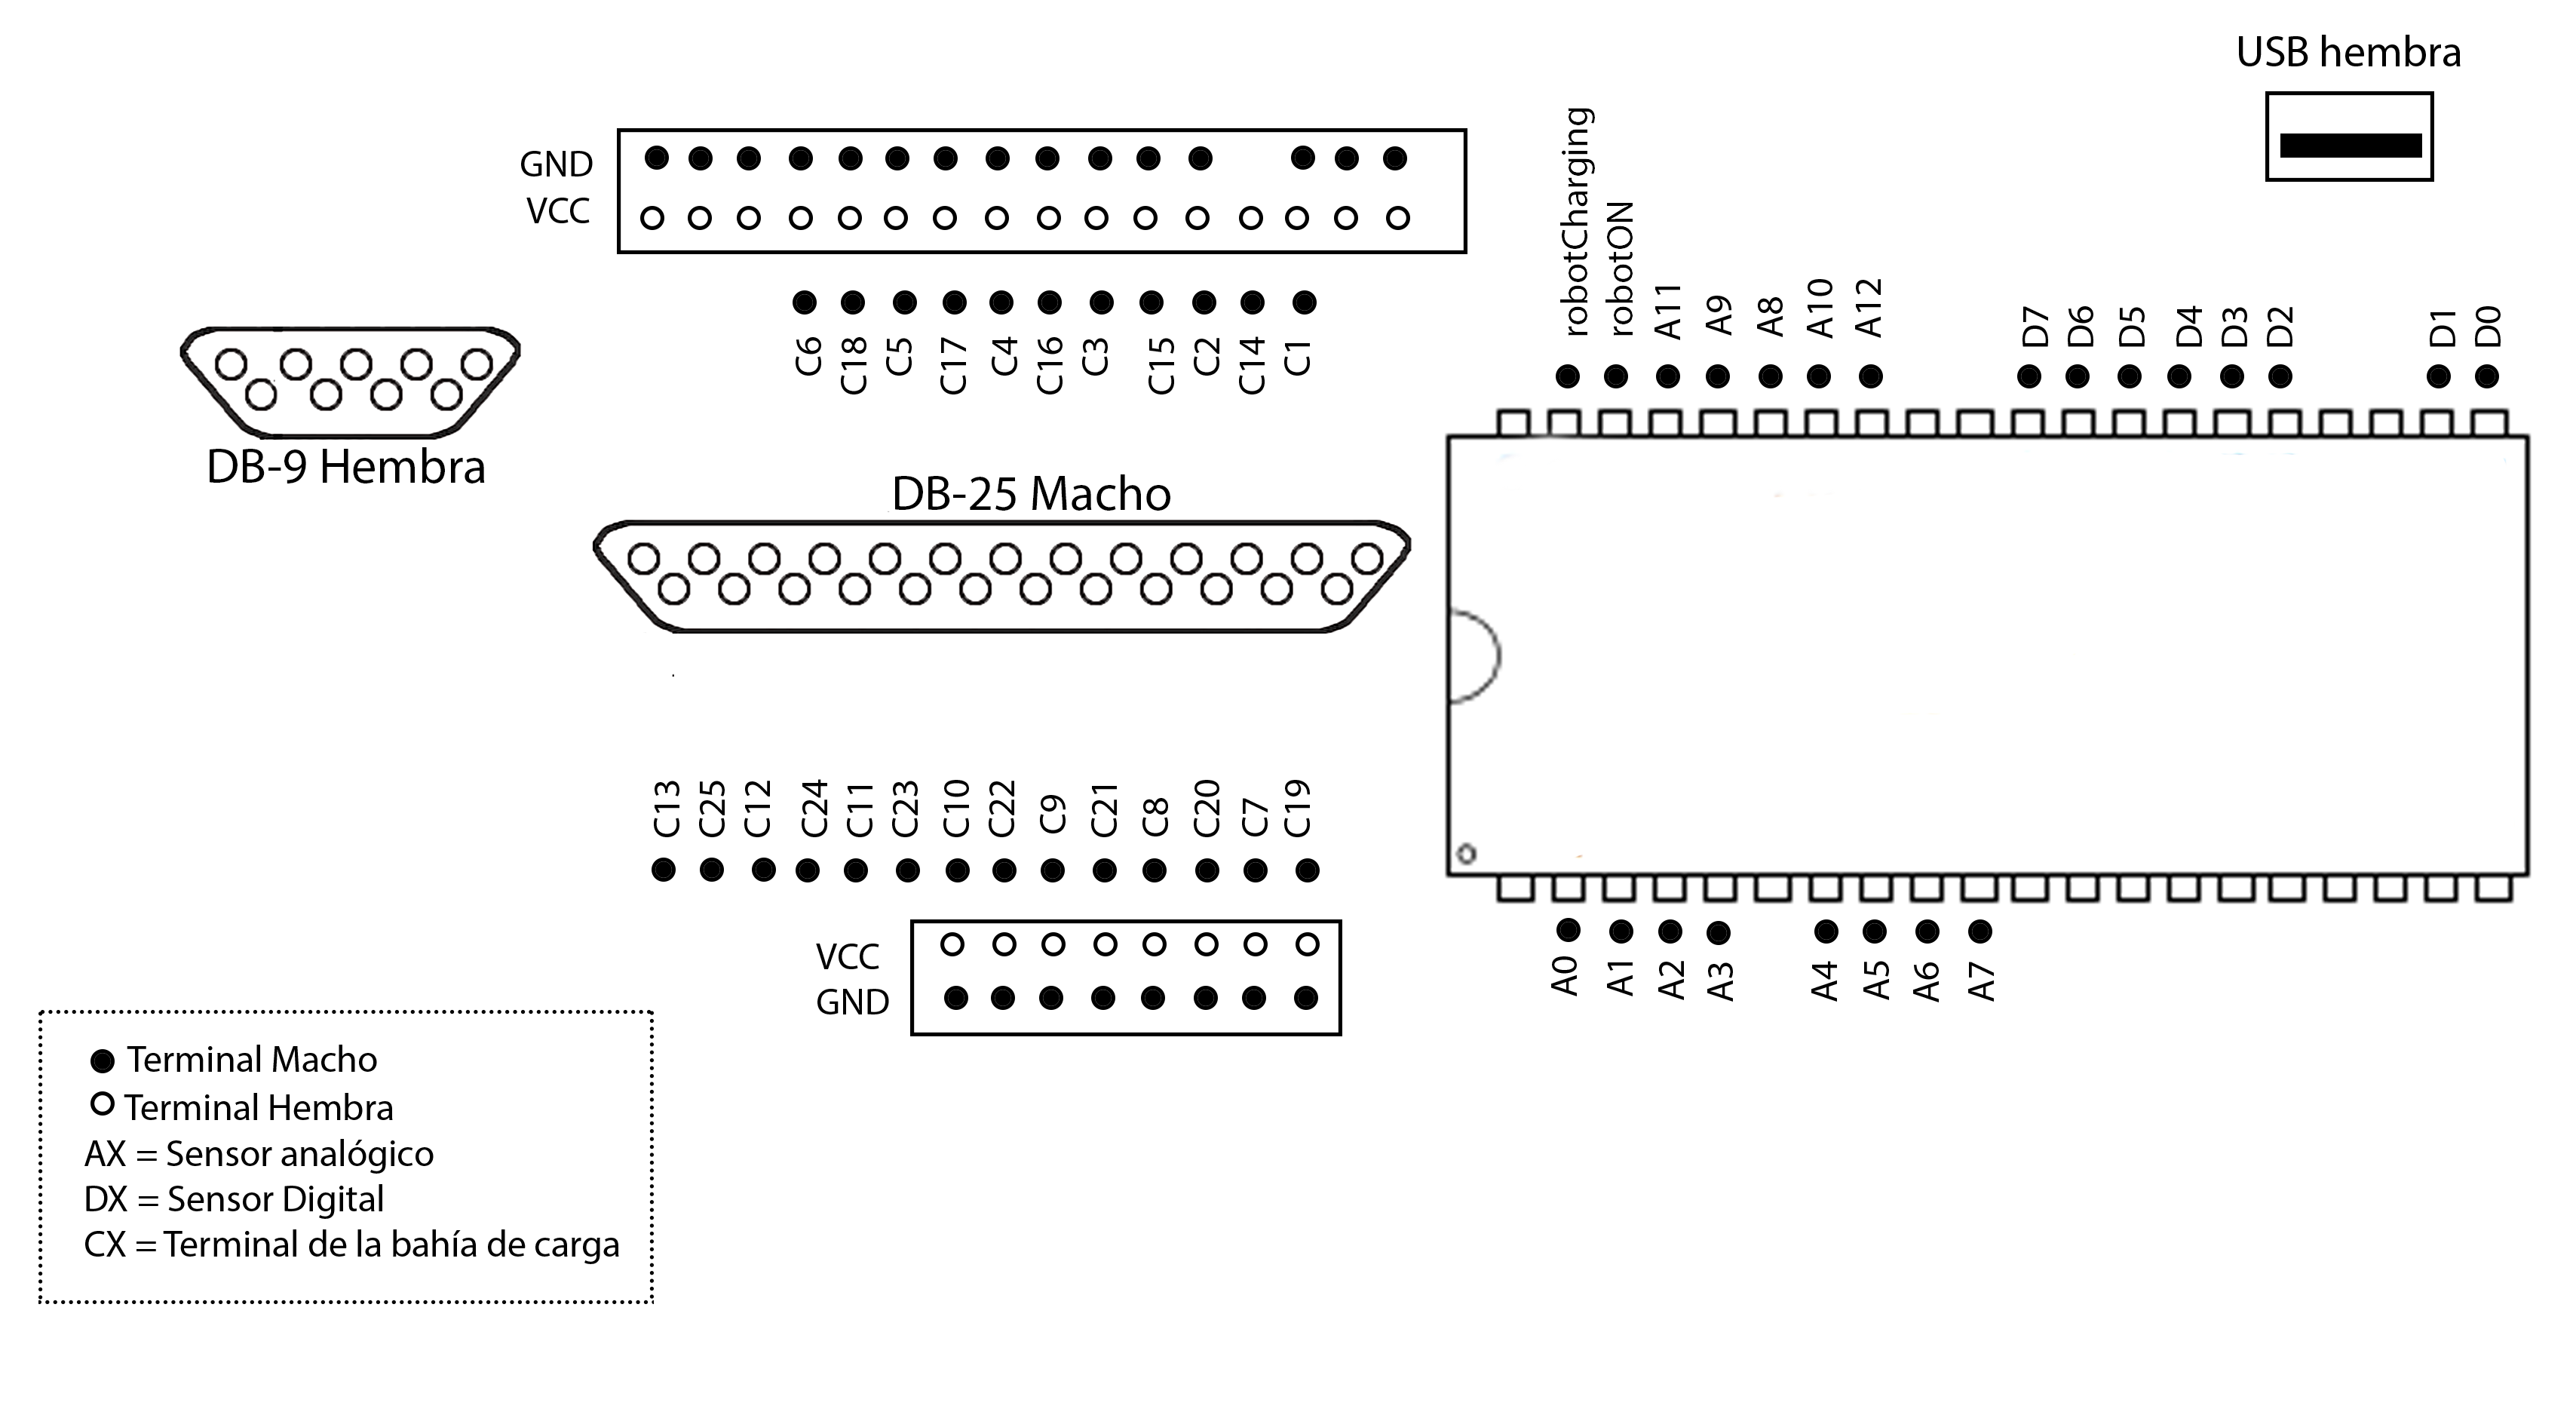
\includegraphics[width=0.8\textwidth]{figures/esquemaPlaca.png}
\caption{Esquema de las terminales en la placa fenólica}
\centering
\label{fig:pcbSchematics}
\end{center}
\end{figure} 

\begin{figure}[h]
\begin{center}
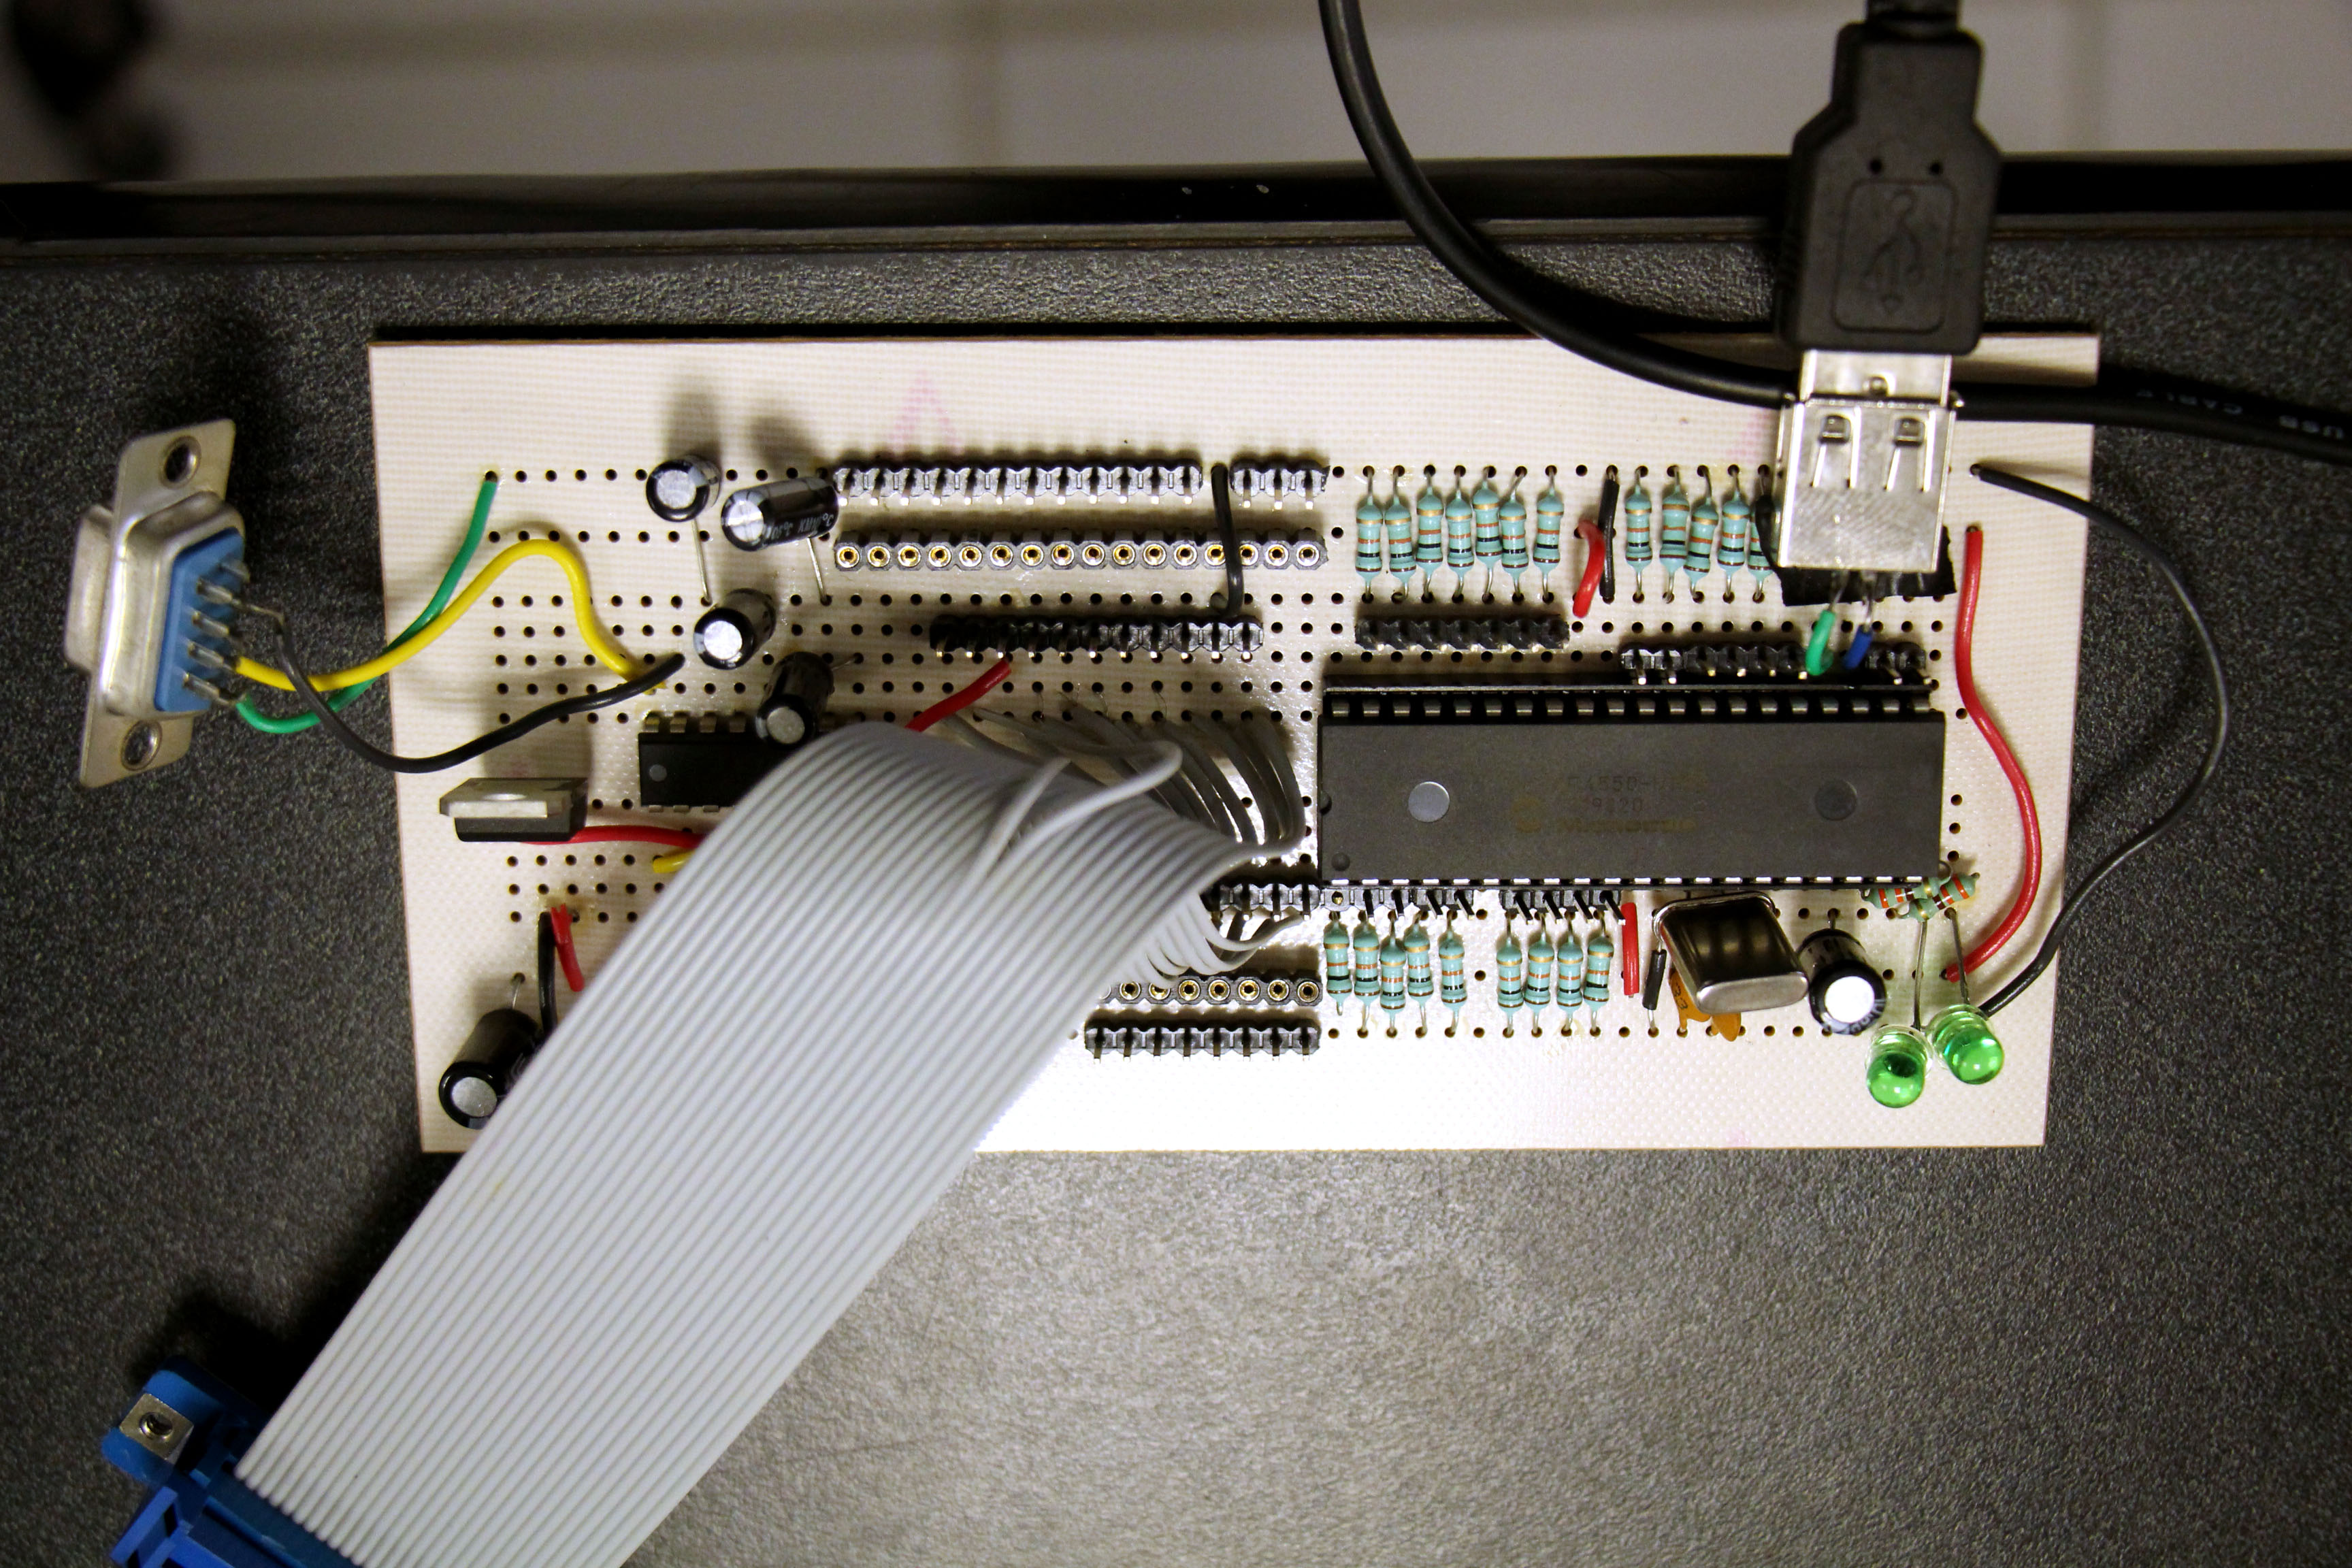
\includegraphics[width=0.8\textwidth]{figures/pcb.jpg}
\caption{Placa fenólica para el uso de UDG\_Create}
\centering
\label{fig:pcb}
\end{center}
\end{figure} 
\section{Conexiones físicas}
Para la correcta ejecución de los programas creados con la biblioteca UDG\_Create es necesario realizar algunas conexiones físicas entre los distintos componentes de hardware.\\
1. Conecte el cable DB-25 macho de la placa fenólica al puerto DB-25 hembra en la bahía de carga del Create\textsuperscript{\textregistered} como se muestra en la figura \ref{fig:cargoCable}.\\
\begin{figure}
\begin{center}
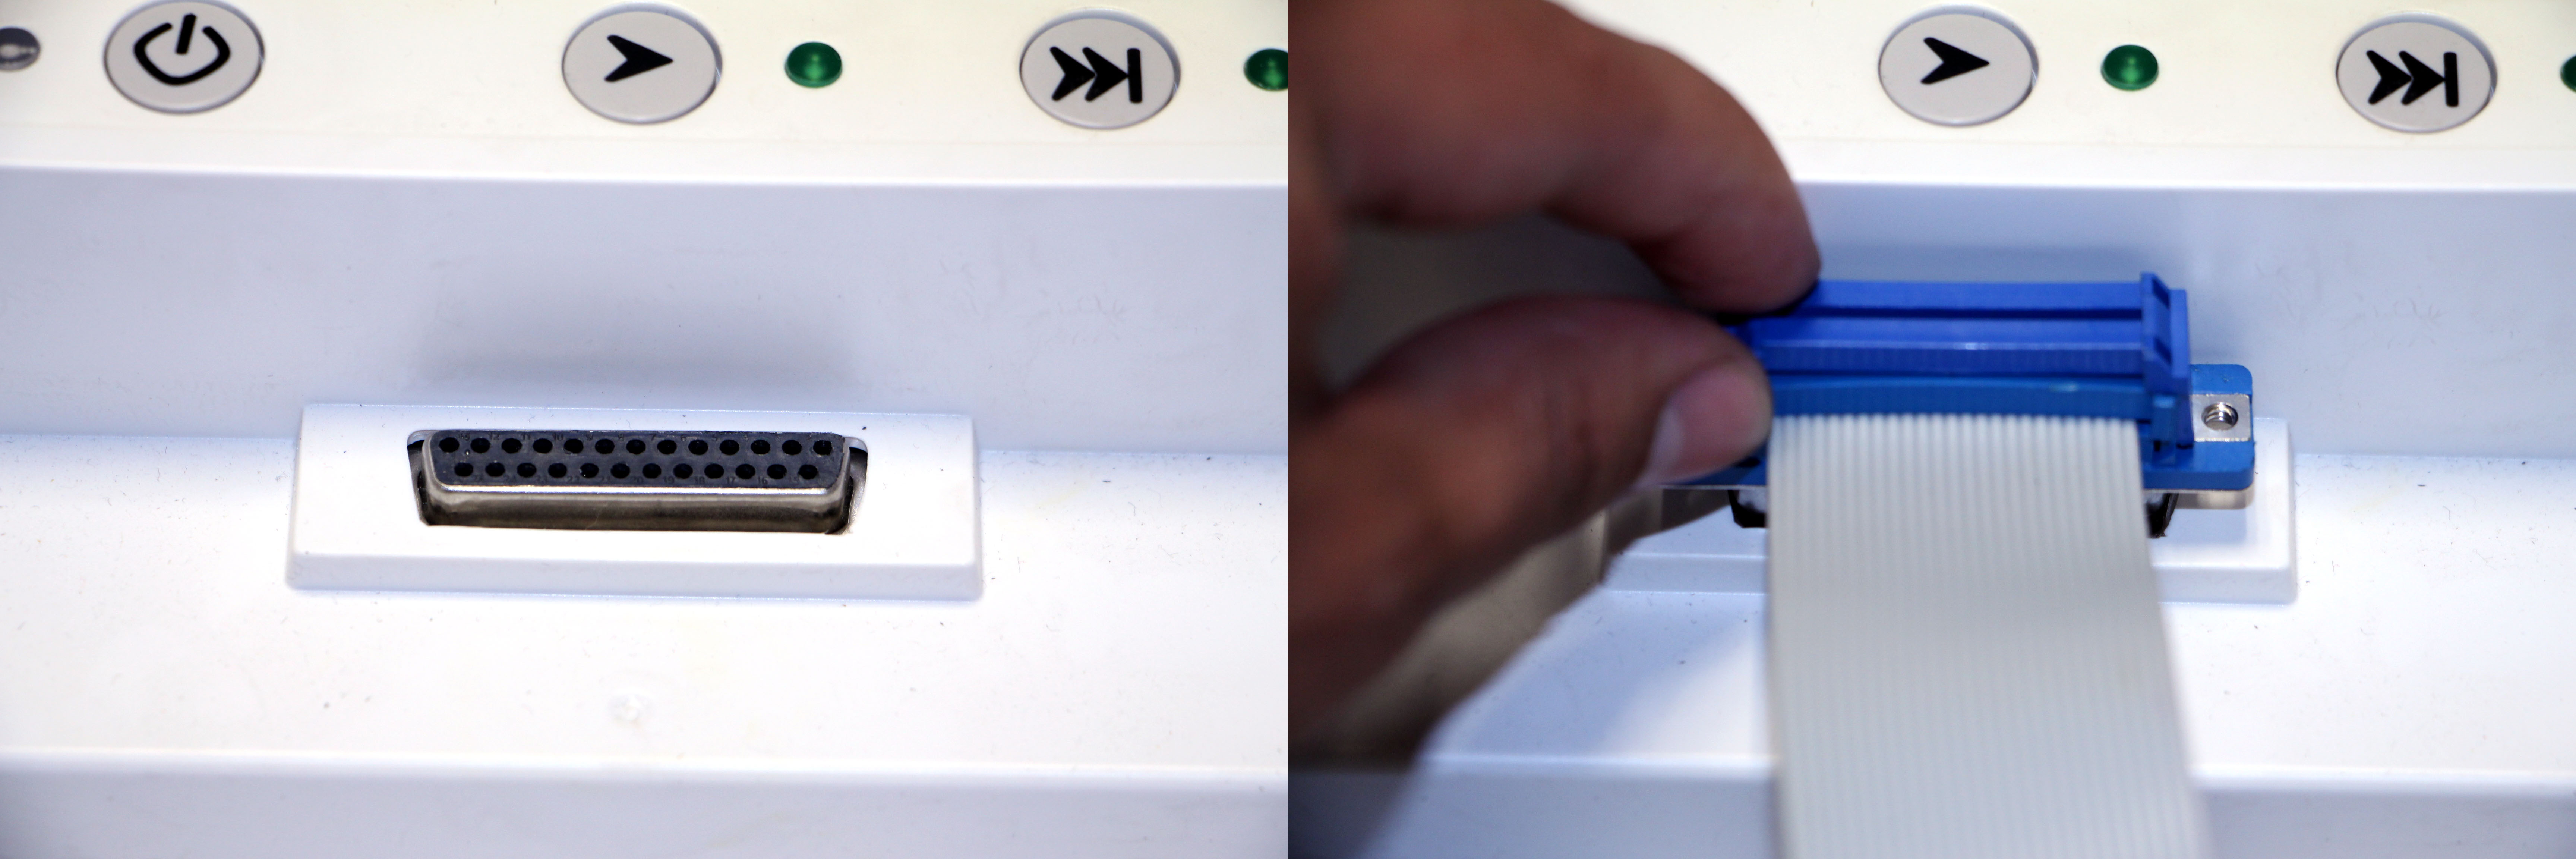
\includegraphics[width=0.8\textwidth]{figures/cargo.jpg}
\caption{Conector DB-25 en la bahía de carga del Create\textsuperscript{\textregistered}}
\centering
\label{fig:cargoCable}
\end{center}
\end{figure} 
2. Conecte un cable USB al puerto puerto correspondiente de la placa fenólica como se muestra en la figura \ref{fig:usbCable}.\\
\begin{figure}
\begin{center}
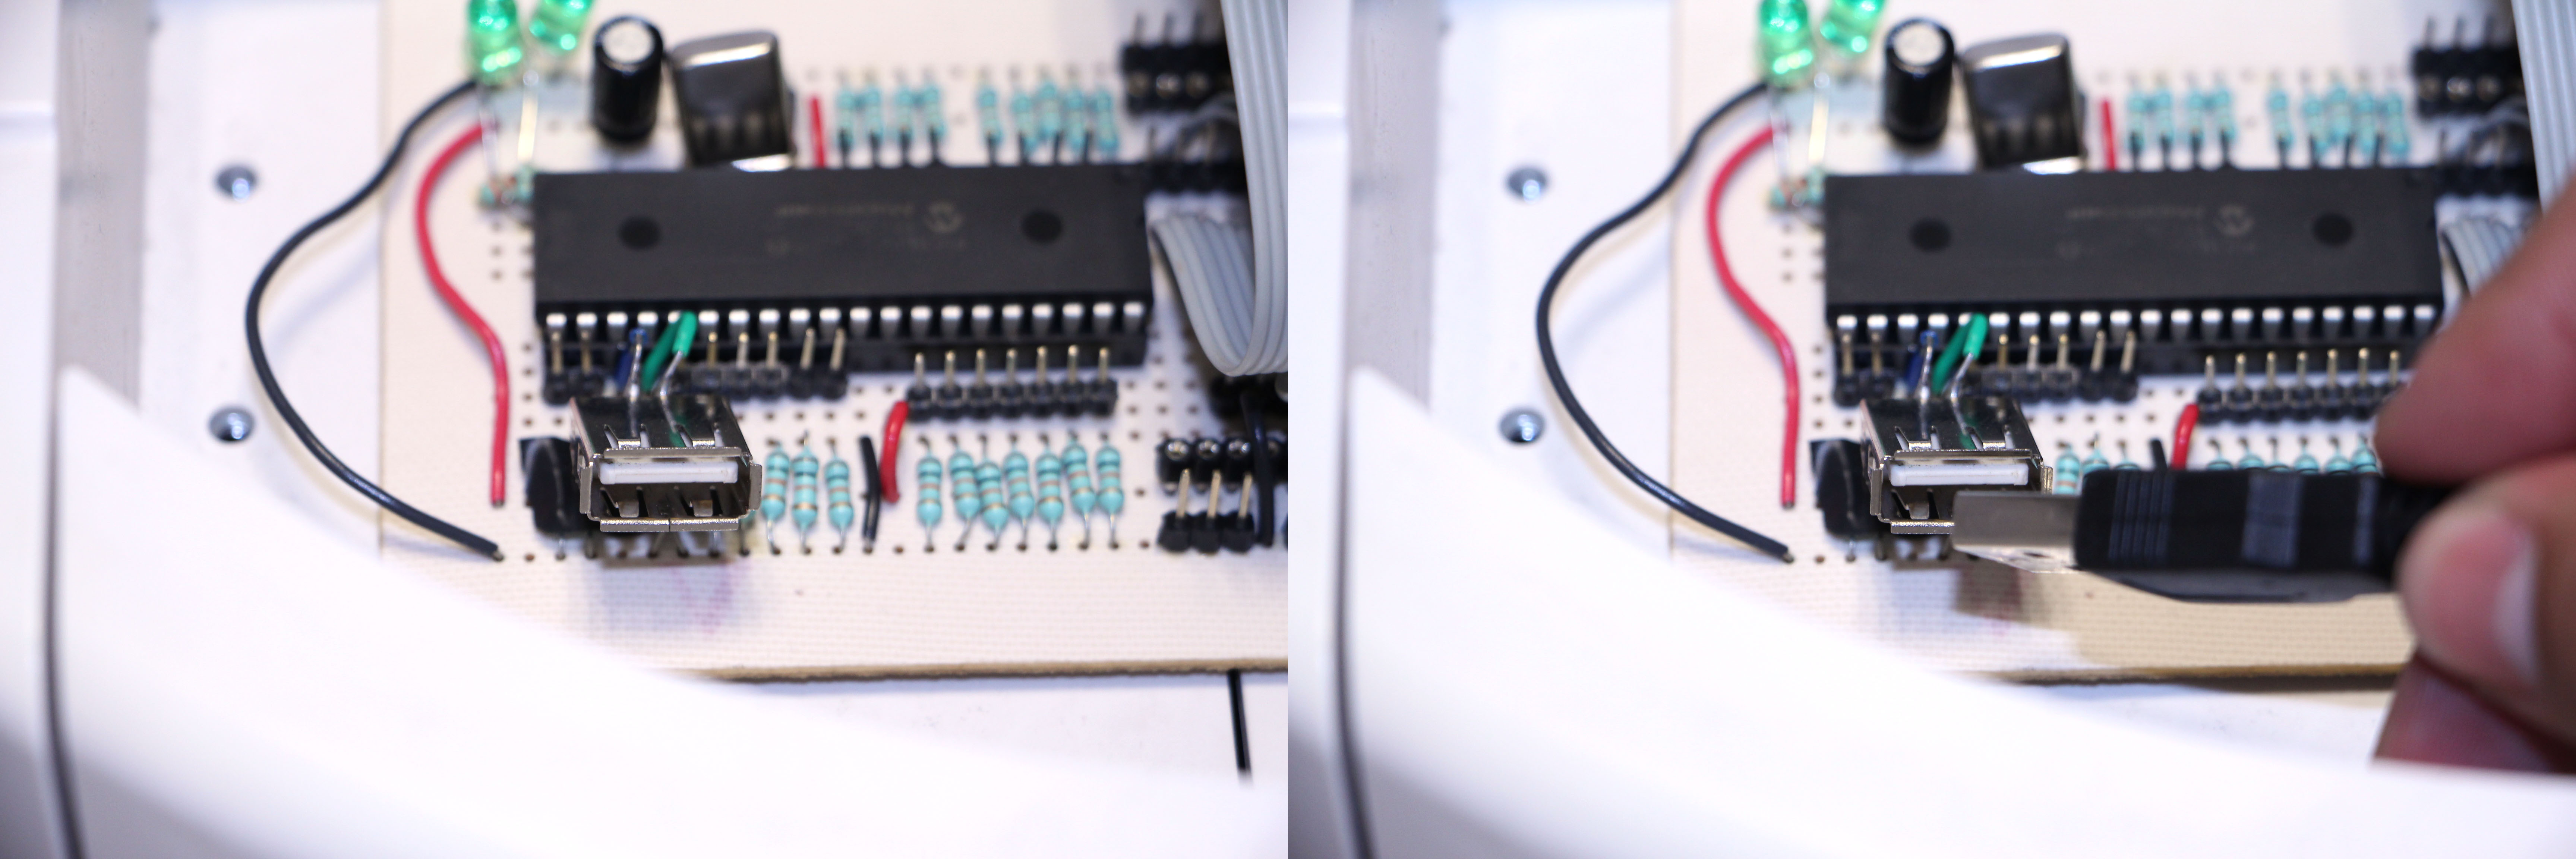
\includegraphics[width=0.8\textwidth]{figures/usbcable.jpg}
\caption{Conexión de los sensores externos mediante un cable USB}
\centering
\label{fig:usbCable}
\end{center}
\end{figure} 
3. Conecte un cable serial al conector DB-9 de la placa fenólica como se ilustra en la figura \ref{fig:serialCable}. Es posible utilizar un convertidor serial/usb si su PC no posee un puerto serial.\\
\begin{figure}
\begin{center}
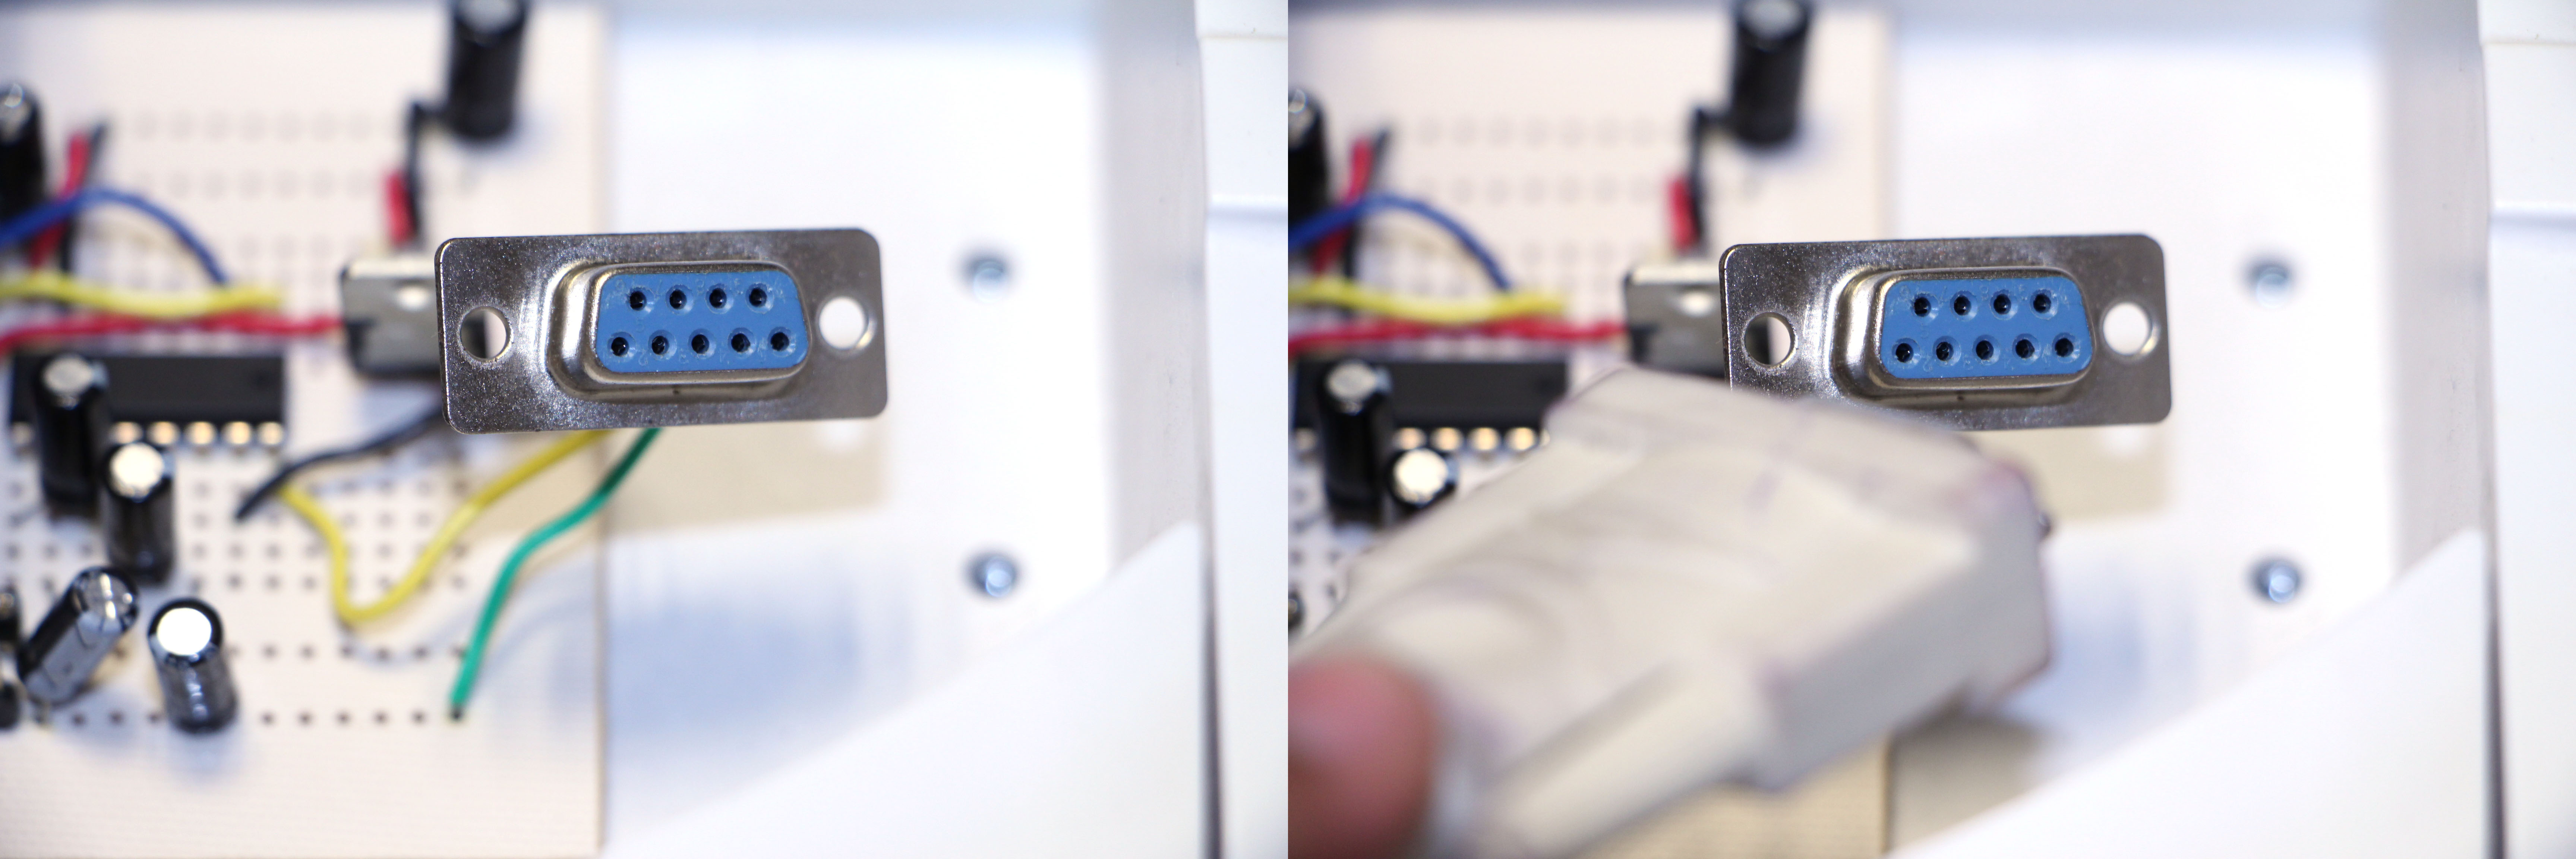
\includegraphics[width=0.8\textwidth]{figures/serialcable.jpg}
\caption{Conector DB-9 para la comunicación serial}
\centering
\label{fig:serialCable}
\end{center}
\end{figure} 
4. Para conectar sensores externos, tanto analógicos como digitales, se recomienda que estos tengan terminales acopladas a las puntas. Por seguridad, la terminal VCC del sensor debe ser macho y el resto hembras (ver figura \ref{fig:cables}). Conecte las terminales de alimentación de los sensores a la placa fenólica. El identificador de sensor en el software será  interpretado de acuerdo a la posición de la conexión física de la terminal de señal. Esto se ilustra en la figura \ref{fig:sensors}.\\
\begin{figure}
\begin{center}
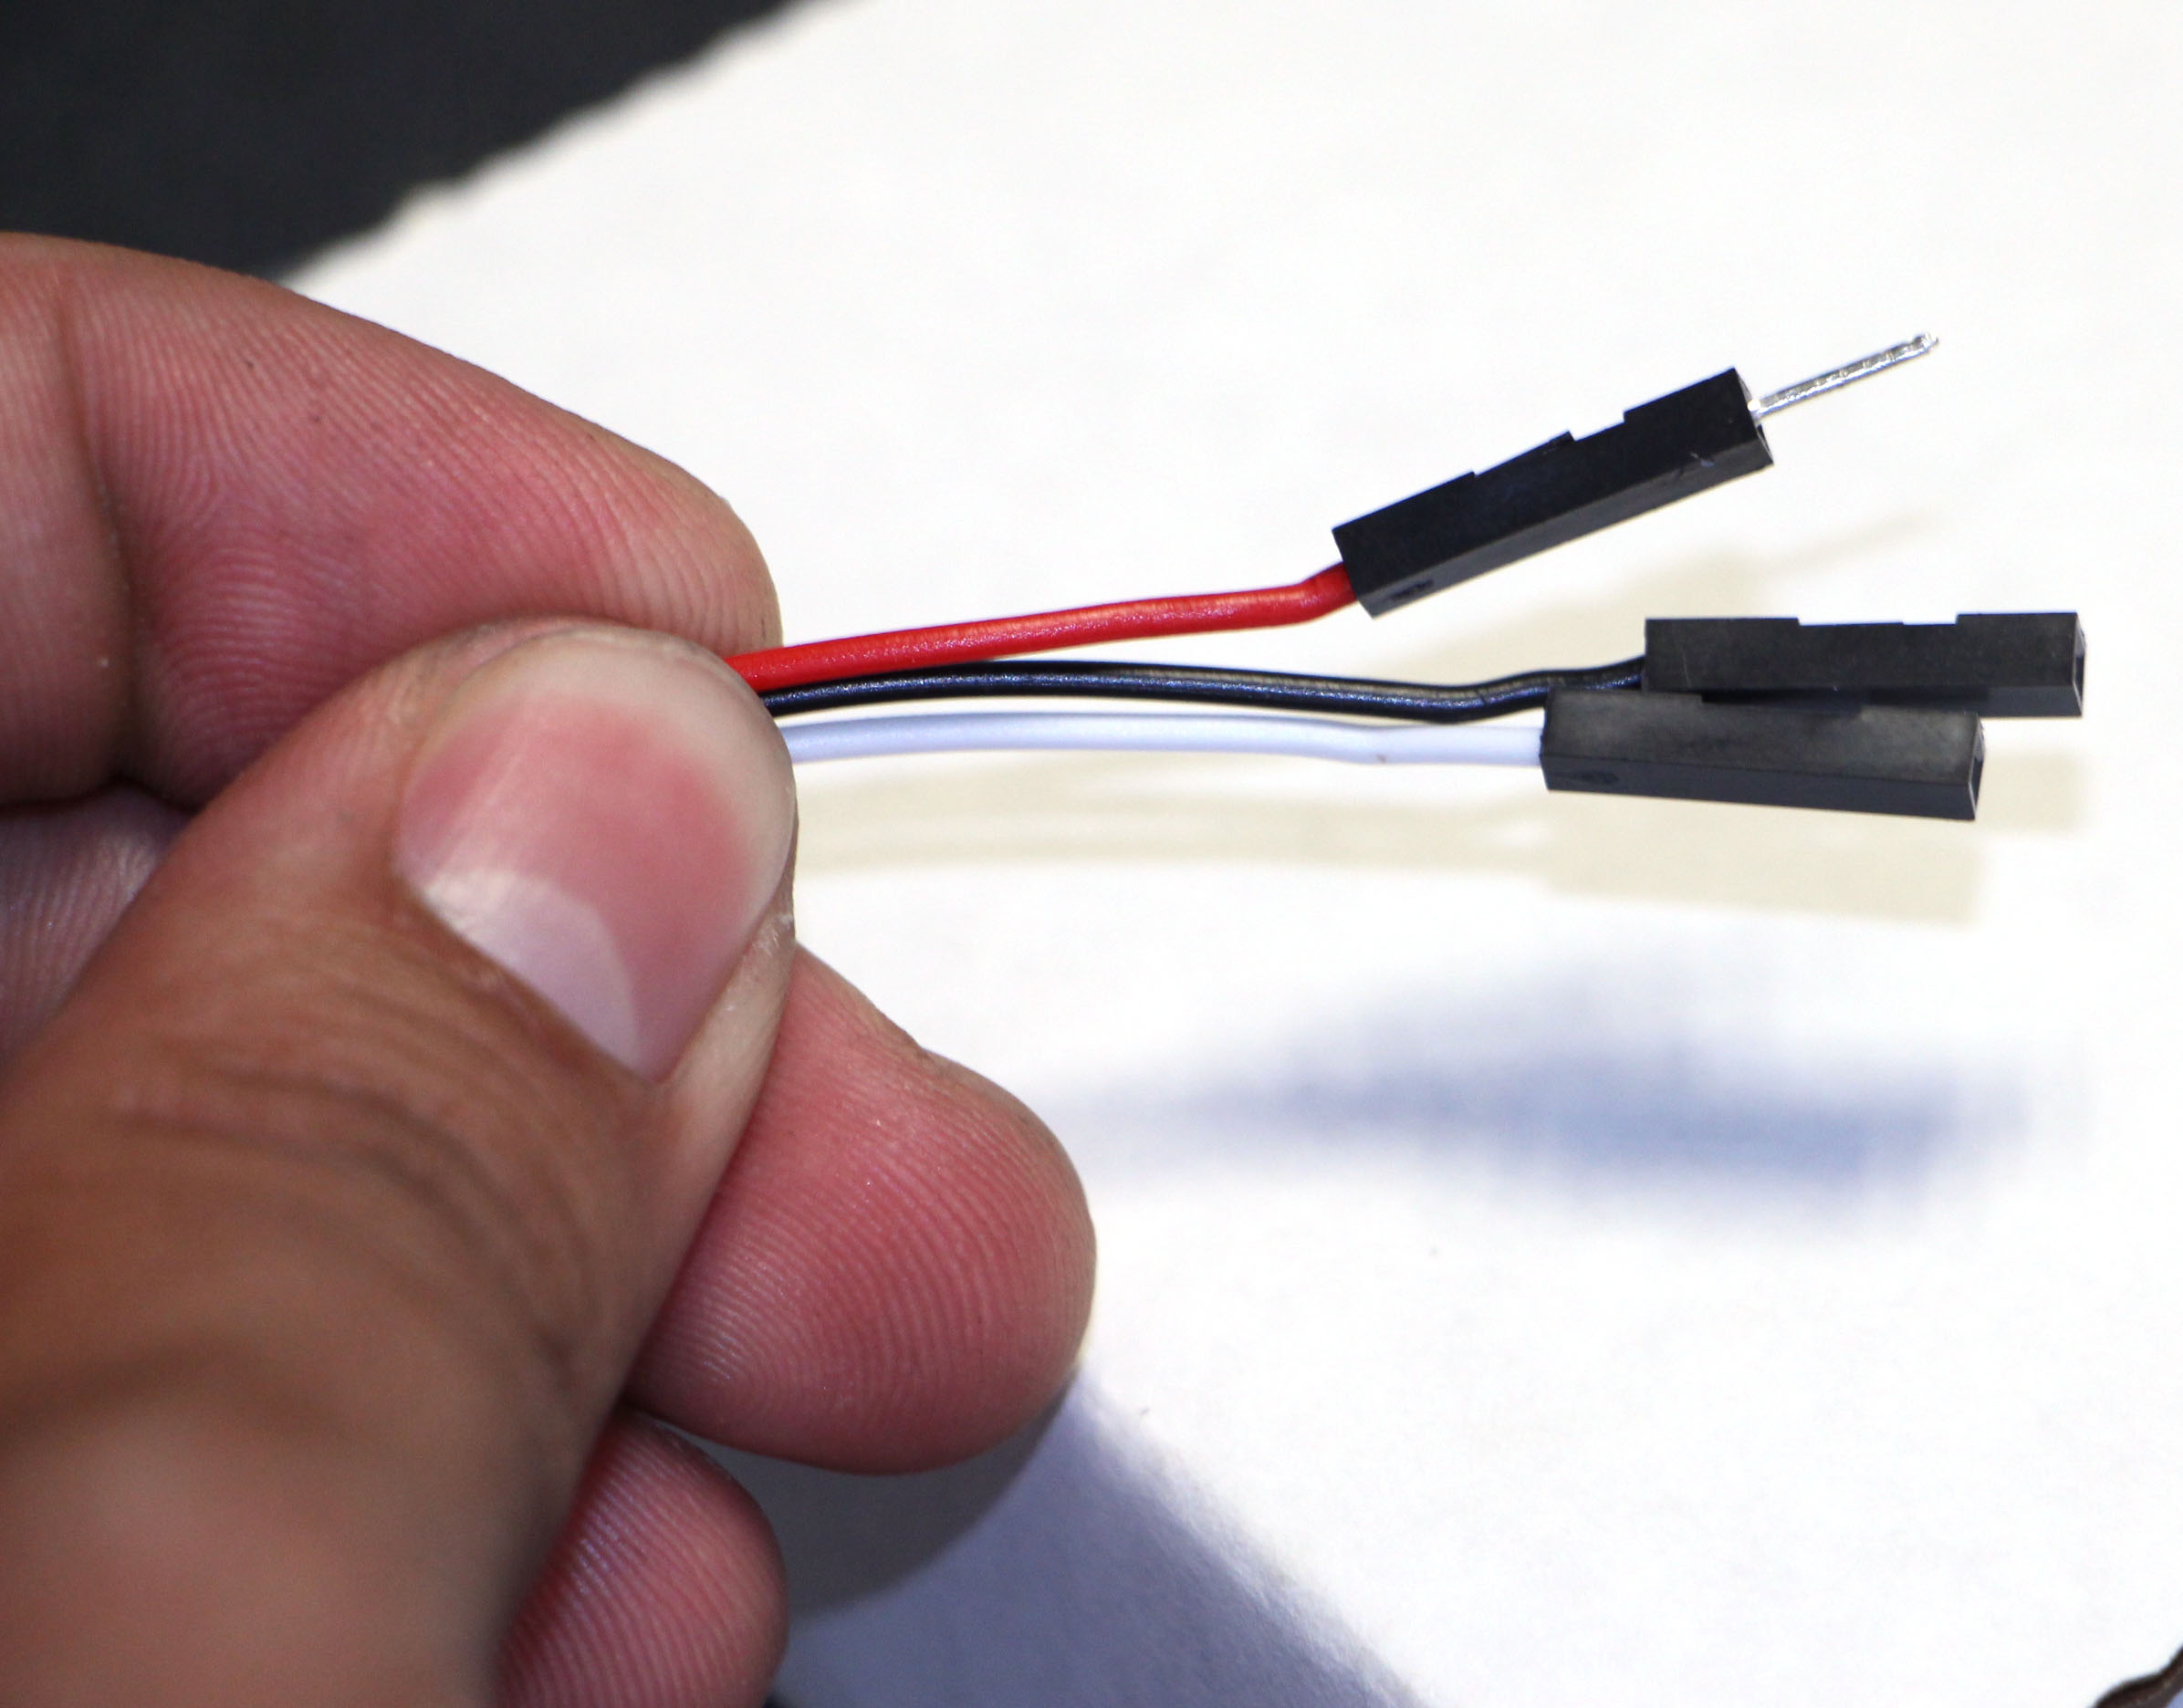
\includegraphics[width=0.8\textwidth]{figures/cables.jpg}
\caption{Terminales para cables recomendadas}
\centering
\label{fig:cables}
\end{center}
\end{figure} 
\begin{figure}
\begin{center}
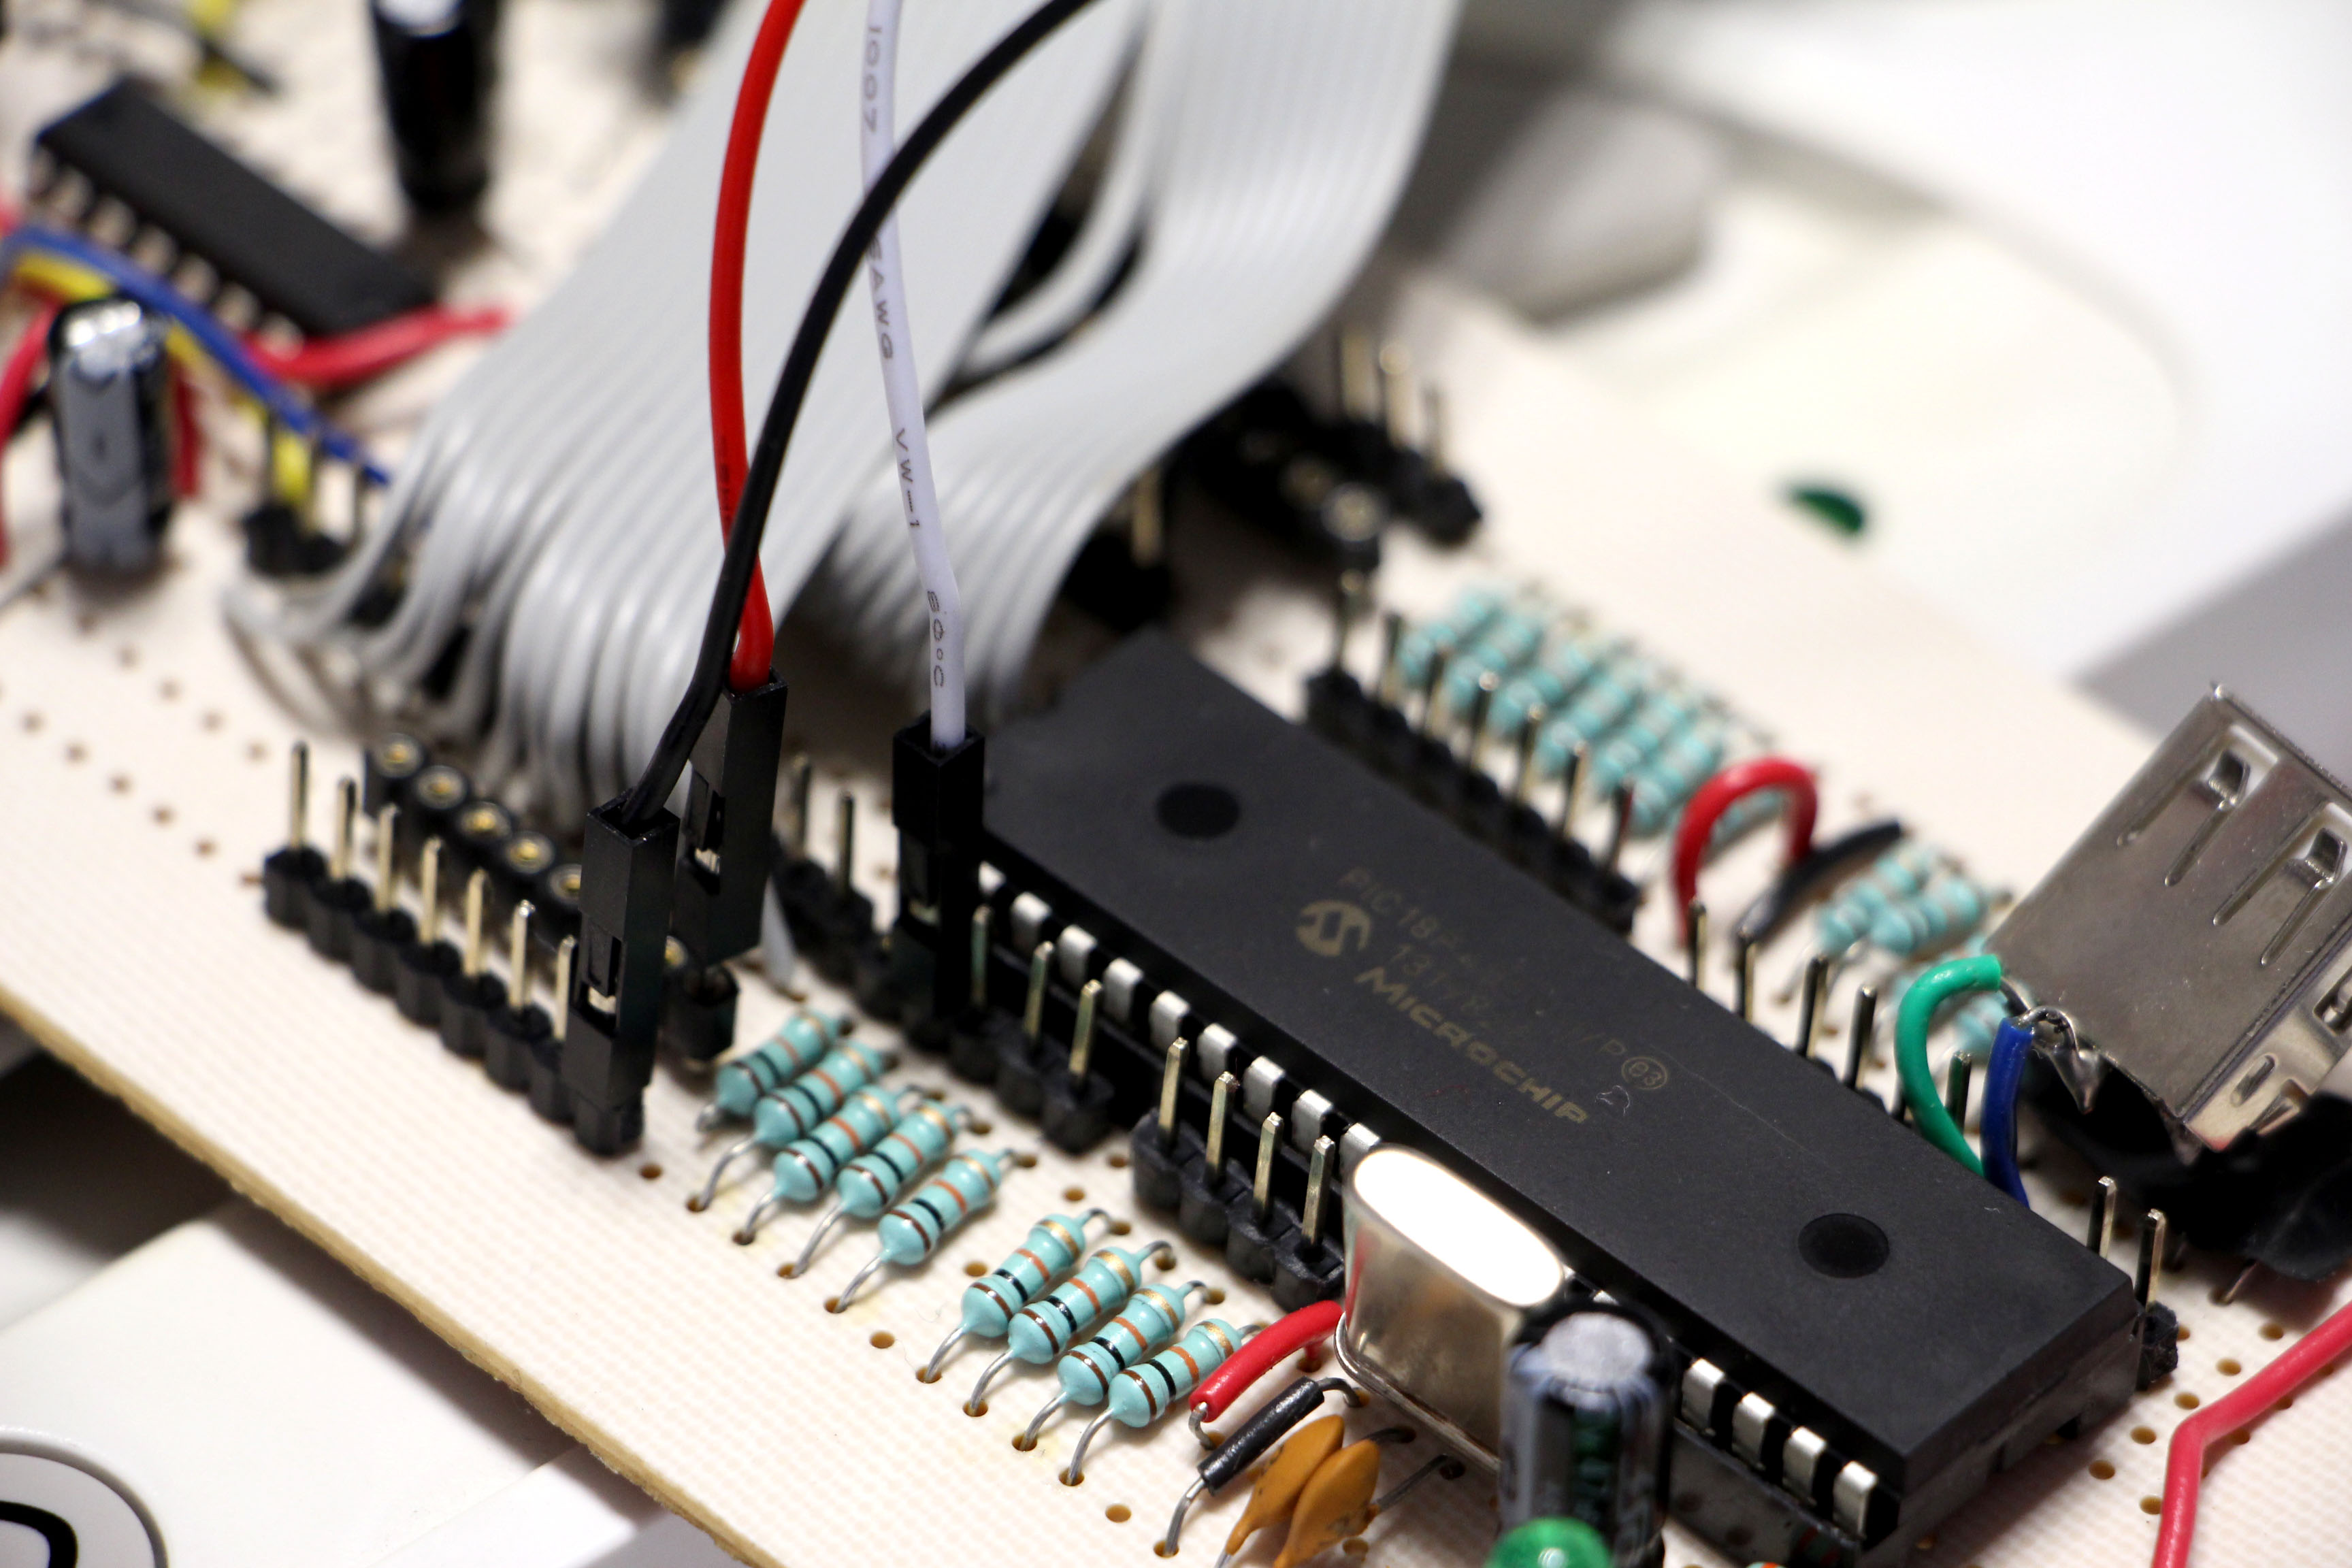
\includegraphics[width=0.8\textwidth]{figures/sensors.jpg}
\caption{Conexión de sensores externos}
\centering
\label{fig:sensors}
\end{center}
\end{figure} 
5. Conecte el otro extremo de los cables serial y USB a la PC (ver figura \ref{fig:computerCables}).\\
\begin{figure}
\begin{center}
\includegraphics[width=0.8\textwidth]{figures/computerCables.jpg}
\caption{Conexión de la placa fenólica a la PC}
\centering
\label{fig:computerCables}
\end{center}
\end{figure} 
6. Una vez realizadas estas conexiones, el robot está listo para usarse. Para aprovechar al máximos las capacidades de la biblioteca UDG\_Create se recomienda utilizar una computadora portátil y montarla junto con los sensores sobre el robot como se muestra en la figura \ref{fig:usage}, sin embargo, otras técnicas como la utilización de hardware intermedio para la comunicación Wi-Fi o Zigbee son también posibles.
\begin{figure}
\begin{center}
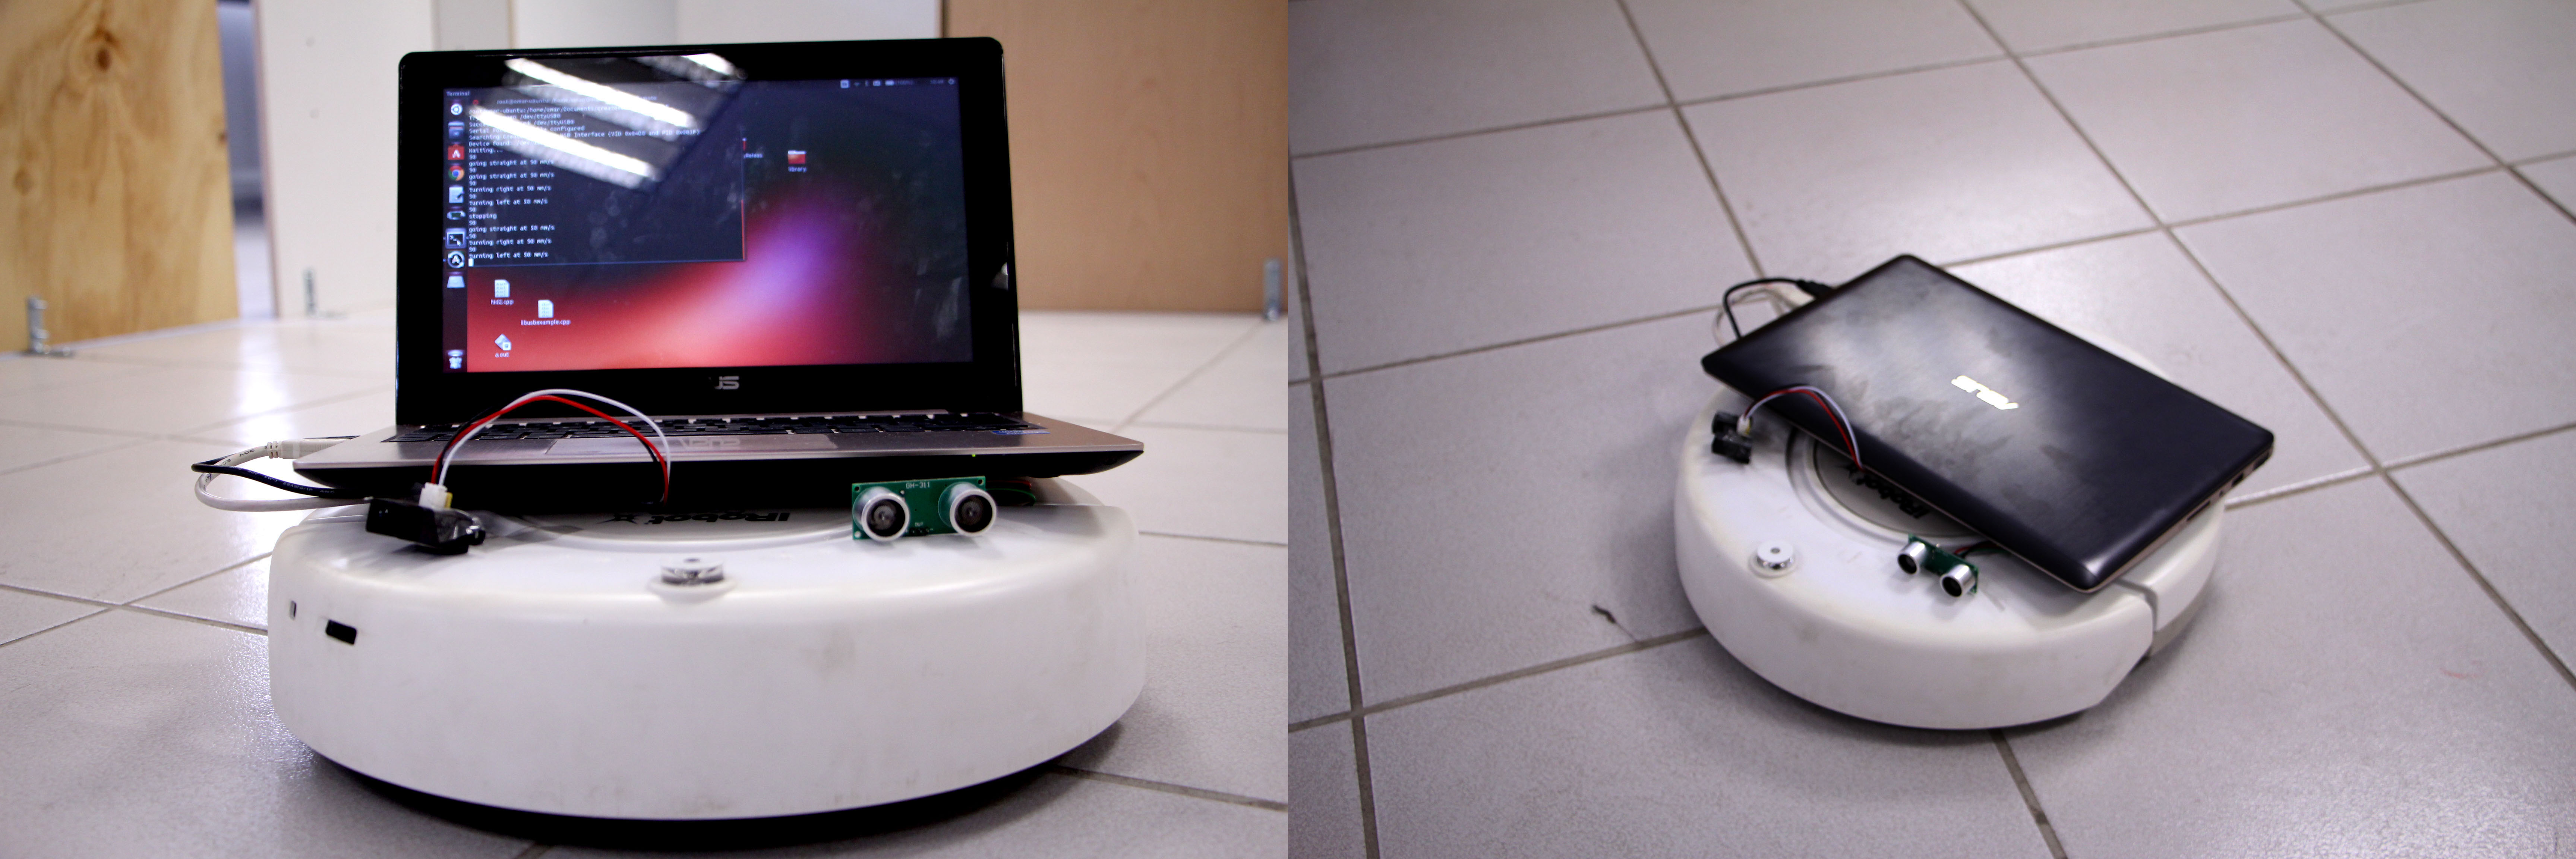
\includegraphics[width=0.8\textwidth]{figures/usage.jpg}
\caption{Modo de uso recomendado}
\centering
\label{fig:usage}
\end{center}
\end{figure} 
\section{Dependencias de software}
Para utilizar la biblioteca UDG\_Create es necesario contar con un sistema operativo basado en linux para la arquitectura x86. Durante la ejecución se requieren permisos de root para la lectura de los sensores externos USB. Para recompilar la biblioteca es necesario contar con un compilador que cumpla con el estándar c++ 11. En esta guía de usuario se utilizan Ubuntu 13.10 y g++ 4.7.
\subsection{Recompilación de la biblioteca con g++}
La biblioteca UDG\_Create se distribuye como una paquete precompilado. Si necesita recompilarla puede hacerlo de manera automática ejecutando el script \emph{rebuildLibrary.sh} contenido en la carpeta del código fuente. Se recomienda utilizar los siguientes comandos:\\
\emph{cd \textless directorio\_del\_codigo\_fuente \textgreater}\\
\emph{sh rebuildLibrary.sh}\\
Para compilaciones personalizadas se requiere llevar a cabo los siguientes pasos:\\
Compilar los archivos fuente (sin ligado).\\
\emph{g++ -c -std=c++11  USBLayer.cpp  ExternalSensors.cpp  UDG\_Create.cpp SerialPort.c }\footnote{Para veriones de g++ 4.3 y posteriores pero inferiores a 4.7 utilizar -std=c++0x en lugar de -std=c++11} \\
Empaquetado del código objeto.\\
\emph{ar rvs UDG\_Create.a ExternalSensors.o  UDG\_Create.o SerialPort.o USBLayer.o}\\
De manera opcional, para utilizar UDG\_Create.h como archivo de encabezado estandar debe agregar el prefijo lib al nombre del paquete.\\
\emph{\emph{ar rvs libUDG\_Create.a ExternalSensors.o  UDG\_Create.o SerialPort.o USBLayer.o}\\}\\
Por último, si asi lo desea, puede eliminar los archivos intermedios generados durante el proceso.\\
\emph{rm *.o}
\section{Uso de UDG\_Create de manera local}
Copie los archivos UDG\_Create.h y UDG\_Create.a al directorio del código fuente de su proyecto.\\
Asegurese de que su programa incluya a la biblioteca como \emph{\#include ``UDG\_Create.h''} (con comillas).\\
Incluya UDG\_Create.a a su comando de compilación para realizar el ligado utilizando la bilioteca. Por ejemplo, para el programa:\\


\begin{lstlisting}[caption={main.cpp}]
#include "UDG_Create.h"
int main()
{
	Create robot;
	robot.demo(9);
	return 0;
}

\end{lstlisting}

Puede utilizar:\\
\emph{g++ main.cpp UDG\_Create.a}

\section{Uso de UDG\_Create como biblioteca estándar}
Copiar UDG\_Create.h a uno de los directorios por defecto para archivos de encabezado (por ejemplo /usr/include/) o usar la opción -I de g++ para especificar la ruta al momento de compilar.\\
Copiar libUDG\_Create.a a uno de los directorios por defecto de c++ para bibliotecas (por ejemplo /usr/lib/) o usar la opción -L de g++ para especificar la ruta en el momento de la compilación.
La biblioteca debe  incluirse en el código fuente como \emph{\#include {\textless}UDG\_Create.h\textgreater} (con paréntesis angulares).\\
Agregue -lUDG\_Create a su comando de compilación para realizar el ligado utilizando la biblioteca. Por ejemplo para el programa\\
\begin{lstlisting}[caption={main.cpp}]
#include <UDG_Create.h>
int main()
{
	Create robot;
	robot.demo(9);
	return 0;
}

\end{lstlisting}

puede usar:
\emph{g++ main.cpp -lUDG\_Create}
\section{La Clase Create}
La clase de c++ Create, esta contenida en el archivo UDG\_Create.h y en ella se describe la abstracción de los sensores, actuadores y otros componentes del robot además de todas las operaciones necesarias para la inicialización y operación de los módulos RS-232 y USB.
\subsection{Tipos de datos y enumeraciones}
\subsubsection{enum errorCodes}
Define los códigos de error para distintas condiciones de falla durante la ejecución de un programa.\\
INVALID\_DEMO (0x00): El número de modo de desmostración seleccionado no existe.\\
INVALID\_BAUDRATE (0x01): Se ha seleccionado una velocidad de transmisión no válida.\\
INVALID\_INSTRUCTION\_MODE (0x02): Se ha intentado ejecutar una instrucción en un modo que no lo permite.\\
OUT\_OF\_RANGE (0x03): El parámetro seleccionado está fuera del rango permitido.\\
INVALID\_MODE (0x04): Se ha seleccionado un modo de operación inexistente.\\

\subsubsection{enum modes}
Enlista los distintos modos en los que puede operar el robot.\\
OFF: Robot apagado.\\
PASSIVE: En el modo pasivo es posible ejectutar los programas de demostración asi como leer y escribir información de sensores, pero no se permite ejecutar comandos de actuadores.\\
SAFE: En el modo seguro se tiene control total del robot, pero este regresa a modo pasivo si se detecta un borde (por el que el robot pudiera caer), se solicita un radio de giro menor al radio del robot o se conecta el cargador.\\
FULL: Se tiene control absouluto del robot.\\
\subsubsection{enum baudCode}
Enumera las velocidades de transmisión soportadas por el Create\textsuperscript{\textregistered}. Las constantes tienen un nombre de la forma BAUDX en donde X representa la velocidad de transmisión en baudios.\\
BAUD300 (0x00).\\
BAUD600 (0x01).\\
BAUD1200 (0x02).\\
BAUD2400 (0x03).\\
BAUD4800 (0x04).\\
BAUD9600 (0x05).\\
BAUD14400 (0x06).\\
BAUD19200 (0x07).\\
BAUD28800 (0x08).\\
BAUD38400 (0x09).\\
BAUD57600 (0x0A).\\
BAUD115200 (0x0B).\\

\subsubsection{enum  chargingstates}
Describe los posibles estados de carga en los que pudiera encontrarse el robot. La documentación del fabricante no proporciona información adicional respecto a estas condiciones, se asumen autoexplicativas.\\
NOT\_CHARGING (0x00).\\
RECONDITIONING\_CHARGING (0x01).\\
FULL\_CHARGING (0x02).\\
TRICKLE\_CHARGING (0x03).\\
WAITING (0x04).\\
CHARGING\_FAULT\_CONDITION (0x05).\\

\subsubsection{enum infraredbytechars}
Define los posibles valores que pudieran recibirse a través del receptor infrarrojo provenientes del control remoto, la base de carga, otros robots o aplicaciones externas. La documentación del fabricante no proporciona información adicional por lo que los valores se asumen autoexplicativos.\\
IRLEFT (0x81).\\
IRFORWARD (0x82).\\
IRRIGHT (0x83).\\
IRSPOT (0x84).\\
IRMAX (0x85).\\
IRSMALL (0x86).\\
IRMEDIUM (0x87).\\
IRLARGE (0x88).\\
IRPAUSE (0x89).\\
IRPOWER (0x8A).\\
IRARC\_FORWARD\_LEFT (0x8B).\\
IRARC\_FORWARD\_RIGHT (0x8C).\\
IRDRIVE\_STOP (0x8D).\\
IRSENDALL (0x8E).\\
IRSEEKDOCK (0x8F).\\
IRRESERVED (0x90).\\
IRRED (0x91).\\
IRGREEN (0x92).\\
IRFORCEFIELD (0x93).\\
IRREDGREEN (0x94).\\
IRREDFORCEFIELD (0x95).\\
IRGREENFORCEFIELD (0x96).\\
IRREDGREENFORCEFIELD (0x97).\\

\subsubsection{ enum VerbosityLevels}
VERBOSITY\_NORMAL (0x00): Los mensajes del robot se escriben a la salida estándar.\\
VERBOSITY\_FILE (0x01): Los mensajes del robot se escriben a un archivo.\\
VERBOSITY\_OFF (0x02): No se escribe ningun mensaje.\\
VERBOSITY\_NUMBER\_OF\_LEVELS (0x03): El número total de niveles.\\

\subsubsection{t\_verbosity}
Tipo de dato enumerado que corresponde a los valores de VerbosityLevels.\\

\subsubsection { enum BoolSigned}
SIGNED (0x01).\\
UNSIGNED (0x02).\\
\subsubsection{ boolSigned}
Tipo de dato enumerado que corresponde a los valores de BoolSigned y se utiliza para indicar si los elementos en un arreglo de bytes debe ser considerado como un número con o sin signo.\\

\subsubsection{ NUMBER\_OF\_SENSORS }
Describe el máximo número de sensores externos que pueden conectarse a la interfaz USB.\\

\subsubsection{int16}
Entero de 16 bits, utilizado para garantizar su tamaño idependientemente del compilador. Su definición exacta es:\\
\begin{lstlisting}
typedef struct int_16
{
	unsigned char H; //High byte
	unsigned char L; //Low byte
} int16;
\end{lstlisting}

\subsection{Miembros (privados)}
\paragraph{std::string portName}\mbox{}\\
Una cadena que indica el nombre del enlace simbólico asociado a la comunicación serial con el robot.
\paragraph{int mode}\mbox{}\\
Un valor definido en la enumeración \emph{oimodes} que indica el modo de operación actual del robot.
\paragraph{bool charging}\mbox{}\\
Una variable lógica que indica si el robot está siendo cargado.
\paragraph{int portDescriptor}\mbox{}\\
El descriptor del puerto asociado a la comunicación serial con el robot.
\paragraph{int baudRate}\mbox{}\\
Un valor perteneciente a la enumeración \emph{baudCode} que indica la velocidad de transmisión utilizada para la comunicación serial.
\paragraph{bool bumpRight}\mbox{}\\
Una variable lógica que indica si el lado derecho del parachoques está siendo presionado.
\paragraph{bool bumpLeft}\mbox{}\\
Una variable lógica que indica si el lado izquierdo del parachoques está siendo presionado.
\paragraph{bool wheelDropRight}\mbox{}\\
Una variable lógica que indica si el sensor de caída de la rueda derecha fué activado.
\paragraph{bool wheelDropLeft}\mbox{}\\
Una variable lógica que indica si el sensor de caída de la rueda izquierda fué activado.
\paragraph{bool wheelDropCaster}\mbox{}\\
Una variable lógica que indica si el sensor de caída de la rueda caster fué activado.
\paragraph{bool wall}\mbox{}\\
Una variable lógica que indica si una pared ha sido detectada.
\paragraph{bool cliffLeft}\mbox{}\\
Una variable lógica que indica si un borde ha sido detectado del lado izquierdo.
\paragraph{bool cliffFrontLeft}\mbox{}\\
Una variable lógica que indica si el sensor de bordes frontal izquierdo ha sido activado.
\paragraph{bool cliffFrontRight}\mbox{}\\
Una variable lógica que indica si el sensor de bordes frontal derecho ha sido activado.
\paragraph{bool cliffRight}\mbox{}\\
Una variable lógica que indica si un borde ha sido detectado del lado derecho.
\paragraph{bool virtualWall}\mbox{}\\
Una variable lógica que indica si una pared virtual ha sido detectada.
\paragraph{bool ld0}\mbox{}\\
Una variable lógica que indica si el \emph{low side driver } 0 está encendido.
\paragraph{bool ld1}\mbox{}\\
Una variable lógica que indica si el \emph{low side driver } 1 está encendido.
\paragraph{bool ld2}\mbox{}\\
Una variable lógica que indica si el \emph{low side driver } 2 está encendido.
\paragraph{bool rightWheel}\mbox{}\\
Una variable lógica que indica si el sensor de sobrecorriente de la rueda derecha ha sido activado.
\paragraph{bool leftWheel}\mbox{}\\
Una variable lógica que indica si el sensor de sobrecorriente de la rueda izquierda ha sido activado.
\paragraph{unsigned char infraredbyte}\mbox{}\\
Una variable de un byte que almacena la información leída a través del receptor infrarrojo.
\paragraph{bool advancebtn}\mbox{}\\
Una variable lógica que indica si el botón \emph{advance} del robot está siendo presionado.
\paragraph{bool playbtn}\mbox{}\\
Una variable lógica que indica si el botón \emph{play} del robot está siendo presionado.
\paragraph{int distance}\mbox{}\\
Una variable entera que indica la distancia recorrida desde la última vez que se consultó.
\paragraph{int angle}\mbox{}\\
Una variable entera que indica el ángulo rotado desde la última vez que se consultó.
\paragraph{unsigned char chargingstate}\mbox{}\\
Un miembro de la enumeración \emph{chargingstates} que describe las condiciones actuales de la carga de la batería.
\paragraph{int voltage}\mbox{}\\
Una variable entera que representa el voltaje en mV en la batería del robot.
\paragraph{int current}\mbox{}\\
La corriente en mA que entra (valores positivos) o sale (valores negativos) de la batería del robot. 
\paragraph{unsigned char batterytemperature}\mbox{}\\
La temperatura de la batería del robot en grados celsius.
\paragraph{int batterycharge}\mbox{}\\
La carga de la batería del robot en mAh.
\paragraph{int batterycapacity}\mbox{}\\
La capacidad aproximada de la batería en mAh.
\paragraph{int wallsignal}\mbox{}\\
Una variable entera que representa la magnitud de la lectura en el sensor de paredes.
\paragraph{int cliffls}\mbox{}\\
Una variable entera que representa la magnitud de la lectura en el sensor de bordes  izquierdo.
\paragraph{int clifffls}\mbox{}\\
Una variable entera que representa la intensidad de la lectura en el sensor de bordes frontal izquierdo.
\paragraph{int clifffrs}\mbox{}\\
Una variable entera que representa la intensidad de la lectura en el sensor de bordes frontal derecho.
\paragraph{int cliffrs}\mbox{}\\
Una variable entera que representa la intensidad de la lectura en el sensor de bordes derecho.
\paragraph{bool digitalinput0}\mbox{}\\
Una variable lógica que indica si existe un nivel de voltaje alto en la entrada digital 0.
\paragraph{bool digitalinput1}\mbox{}\\
Una variable lógica que indica si existe un nivel de voltaje alto en la entrada digital 1.
\paragraph{bool digitalinput2}\mbox{}\\
Una variable lógica que indica si existe un nivel de voltaje alto en la entrada digital 2.
\paragraph{bool digitalinput3}\mbox{}\\
Una variable lógica que indica si existe un nivel de voltaje alto en la entrada digital 3.
\paragraph{bool baudchangerate}\mbox{}\\
Una variable lógica que indica si hay un nivel de voltaje alto en la terminal correspondiente al cambio de velocidad de transmsión (terminal 15).
\paragraph{int cargoanalogsignal}\mbox{}\\
Una variable entera que representa el valor de la señal analógica en la terminal 4 del robot.
\paragraph{bool homebase}\mbox{}\\
Una variable lógica que indica si existe una conexión entre el robot y la base de carga.
\paragraph{bool internalcharger}\mbox{}\\
Una variable lógica que indica si el cargador interno está conectado.
\paragraph{unsigned char oimode}\mbox{}\\
Representa el modo de operación actual del robot como un miembro de la enumeracion \emph{oimodes}.
\paragraph{unsigned char songnumber}\mbox{}\\
Indica el número de la canción actualmente seleccionada.
\paragraph{bool songplaying}\mbox{}\\
Indica si hay una canción siendo tocada actualmente.
\paragraph{unsigned char streampackets}\mbox{}\\
El número de sensores o paquetes de sensores solicitados como parte de un flujo.
\paragraph{int reqvelocity}\mbox{}\\
La velocidad de las ruedas solicitada en la última llamada a una instrucción \emph{drive}.
\paragraph{int reqradius}\mbox{}\\
El radio de giro solicitado en la última llamada a una función \emph{drive}.
\paragraph{int reqrvelocity}\mbox{}\\
La velocidad de la rueda derecha solicitada en la última llamada a una función \emph{drive}.
\paragraph{int reqlvelocity}\mbox{}\\
La velocidad de la rueda izquierda solicitada en la última llamada a una función \emph{drive}.
\paragraph{bool streamingState}\mbox{}\\
Una variable lógica que indica si un flujo de paquetes de sensores se está transmitiendo actualmente.
\paragraph{bool externalSensorsEnabled}\mbox{}\\
Una variable lógica que inidica si los sensores externos conectados por usb están actualmente habilitados.
\paragraph{t\_verbosity robotVerbosity}\mbox{}\\
Indica el tipo de mensajes de depuración que se mostrarán en pantalla.


\subsection{Funciones}
\subsubsection{Publicas}
\paragraph{Create()}
Es el método constructor por defecto, inicializa el puerto serial utilizando los primeros enlaces símbolicos para puerto serial y USB disponibles.

\paragraph{Create( std::string \_portName, t\_verbosity verbosityLevel )}\mbox{}\\
\emph{\_portName: }El nombre del enlace símbolico a utilizar para la comunicación serial.\\
\emph{verbosityLevel: } El tipo de mensajes de depuración a recibir durante la ejecución. Los valores disponibles para este parametro son\\
VERBOSITY\_NORMAL: Los mensajes se imprimen a la salida estándar.\\
VERBOSITY\_OFF: No se imprimen mensajes.\\

\paragraph{\char126Create()}\mbox{}\\
Es el método destructor por defecto, libera todos los recursos solicitados durante la ejecución.\\

\paragraph{std::string getPortName()}\mbox{}\\
Regresa un valor de tipo std::string conteniendo el nombre del enlace simbólico utilizado para la inicialización del puerto serial.

\paragraph{void start()}\mbox{}\\
Prepara al robot para recibir instrucciones por el puerto serial y lo pone en modo pasivo (\emph{passive}).\\

\paragraph{void baud(unsigned char baudRate)}\mbox{}\\
\emph{baudRate: } La nueva velocidad de transmisión de acuerdo a los valores establecidos en la Create Open Interface.\\\\
Modifica por software la velocidad de transimisión (baud rate) utilizado para la comunicación serial.  Se recomienda utilizar los miembros de la enumeración baudRate de la forma BAUDx en donde x representa la velocidad.\\

\paragraph{void control()}\mbox{}\\
Pone al robot en modo seguro (safe). Esta función se conserva para mantener compatibilidad con Roomba, se recomienda el uso de la función safe() en su lugar para el Create\textsuperscript{\textregistered}.\\
		
\paragraph{void safe()}\mbox{}\\
Pone al robot en modo seguro (safe).\\

\paragraph{void full()}\mbox{}\\
Pone al robot en modo íntegro (full).\\

\paragraph{void spot()}\mbox{}\\
Ejecuta la demostración ``spot demo'' en la que el robot se mueve formando una espiral. Al terminar de ejecutar la instrucción el Create\textsuperscript{\textregistered} pasa a modo pasivo (passive).\\

\paragraph{void cover()}\mbox{}\\
Ejecuta la demostración ``cover'' de la Create Open Interface en el que se cubre el área de una habitación.\\

\paragraph{void coverAndDock()}\mbox{}\\
Ejecuta la demostración ``cover and dock'' de la Create Open Interface.

\paragraph{void demo( unsigned char demo )}\mbox{}\\
\emph{demo: } El número de la demostración a ejecutar.\\\\
Ejecuta la demostración indicada por \emph{demo}. El número de demo debe estar entre 1 y 9.\\
\paragraph{void drive( int velocity, int radius )}\mbox{}\\
\emph{speed: } La velocidad promedio a la que girarán las ruedas del robot en mm/s.\\
\emph{radius: }Radio en milimetros del giro del robot medido desde el centro del circulo de giro hasta el centro del Create\textsuperscript{\textregistered}.\\\\

Controla las ruedas del robot y lo hace avanzar usando la velocidad y radio especificados. Un radio negativo genera un giro en el sentido de las manecillas del reloj y uno positivo hacia el lado contrario. Valores positivos de velocidad impulsan al robot hacia adelante mientras que los negativos lo hacen hacia atras. Solo los 16 bits menos significativos de los parámetros de entrada son considerados.\\

\paragraph{void driveDirect( int rightVelocity, int leftVelocity )}\mbox{}\\
\emph{rightVelocity: }La velocidad de la rueda derecha.\\
\emph{leftVelocity: }La velocidad de la rueda izquierda.\\\\

Hace al robot avanzar utilizando las velocidades especificadas para las ruedas izquierda y derecha. Valores positivos representan movimiento hacia adelante mientras que los negativos lo hacen hacia atrás. Solo los 16 bits menos significativos del entero con signo son considerados.\\

\paragraph{void leds( unsigned char bit,unsigned char color, unsigned char intensity )} \mbox{}\\
\emph{bit: }Indica el LED a encender. Los valores posibes son:\\
0 = ninguno.\\
2 = Play.\\
8 = Advance.\\
10 = Play y Advance.\\
\emph{color: } Indica el color que mostrará el LED \emph{Power}. El 0 representa color verde y 255 rojo. Valores intermedios mostrarán tonos intermedios (amarillo, naranja, etc).\\
\emph{intensity: }La intensidad con la que encenderá el LED Power.\\\\

Enciende o apaga los diodos LED seleccionados del Create\textsuperscript{\textregistered} permitiendo modificar el color e intensidad del LED Power.\\

\paragraph{void digitalOutputs(unsigned char outputBits)}\mbox{}\\
\emph{outputBits: } El valor de salida deseado.\\
Establece el valor indicado en las 3 terminales de salida del conector DB-25.\\\\
\textbf{Precaución: }Cuando se enciende el robot, las salidas digitales permanecen en nivel alto durante 3 segundos.\\\\

\paragraph{	void pwmLowSideDrivers( unsigned char dirver1, unsigned char driver1, unsigned char driver0)}\mbox{}\\
\emph{driver2: } El ciclo de trabajo para la salida PWM en la terminal 24 del conector DB-25 con un valor de entre 0 y 128.\\
\emph{driver1: } El ciclo de trabajo para la salida PWM en la terminal 22 del conector DB-25 con un valor de entre 0 y 128.\\
\emph{driver0: } El ciclo de trabajo para la salida PWM en la terminal 23 del conector DB-25 con un valor de entre 0 y 128.\\\\

Proporciona el ciclo de trabajo especificado en las salidas de PWM del robot. Este debe ser indicado como un número entero entre 0 y 128, por ejemplo, para indicar un ciclo de trabajo de 25\% en alguna de las salidas se escoje un 32.\\

\paragraph{void lowSideDrivers(unsigned char bits)}\mbox{}\\
\emph{bits: } Indica los bits a activar.\\\\
Activa los bits seleccionados de los \emph{low side drivers}.

\paragraph{void sendIr(unsigned char byteValue)}\mbox{}\\
\emph{byteValue: }El valor del byte  a enviar.\\\\
Esta función envía a un LED infrarrojo conectado a la terminal 23, el byte indicado en el formato esperado por el receptor infrarrojo del robot.\\

\paragraph{	void song(unsigned char,unsigned char,...)}\mbox{}\\
Permite almacenar una canción en la memoria del robot para ser tocada posteriormente. La lista de parametros de entrada es de tamaño variable y debe apegarse al siguiente formato:

\emph{song(numeroDeCancion,numeroDeNotas, nota1,duracion1, nota2, duracion2,...,notaN, duracionN)}\\
\emph{numeroDeCancion} debe tener un valor de entre 0 y 15. \emph{numeroDeNotas} debe estar entre 1 y 16. La altura de \emph{notaX} se apega al esquema de numeración MIDI, pero solo en el rango de entre 31 y 127, cualquier otro valor se considerará como un silencio. El valor de \emph{duracionX} puede estar entre 0 y 255, representando incrementos de 1/64 de segundo.\\

\paragraph{void playSong(unsigned char songNumber)}\mbox{}\\
\emph{songNumber: } El número de canción a tocar.\\\\
Toca la canción previamente grabada mediante la instruccion \emph{song}. Se debe esperar a que termine una canción antes de poder tocar otra.\\

\paragraph{int sensors(unsigned char idPacket)}\mbox{}\\
\emph{idPacket: } El identificador del paquete solicitado.\\\\
Permite obtener el valor del sensor o paquete de sensores seleccionado y actualizar su valor en la variable correspondiente. El valor de retorno es el del último sensor leído.\\

\paragraph{int getSizePacket(int idPacket)}\mbox{}\\
\emph{packet: } El identificador del paquete solicitado.\\\\
Regresa el número de bytes que se esperan del sensor o paquete de sensores específicado.\\

\paragraph{void stream(unsigned char* destinationBuffer,void* thread,int n,...)}\mbox{}\\
\emph{destinationBuffer: } Una apuntador a un buffer de bytes en donde se almacenará la respuesta  a la petición de paquetes.\\
\emph{thread: } Este parametro se conserva para mantener compatibilidad con una versión anterior de la biblioteca y será eliminado a corto plazo.\\
\emph{n: } El número de sensores o paquetes de sensores solicitados. Debe estar entre 0 y 42.\\
\emph{... :} Una lista de tamaño variable conteniendo los identificadores (entre 0 y 42) de los sensores o paquetes de sensores solicitados.\\\\

Esta función indica al robot que debe enviar un flujo de bytes con las lecturas de los sensores solicitados cada 15 ms a través de la conexión serial. Esta información es almacenada en el buffer proporcionado en el formato:\\

19 nbytes IDPaquete1 DatosPaquete1 IDPaquete2 DatosPaquete2 ... IDPaqueteN DatosPaqueteN Checksum

Para más información consulte la instrucción ``stream'' de la Create Open Interface.\\

\paragraph{void pauseResumeStream(bool streamState)}\mbox{}\\
\emph{streamState: } una variable lógica que indica si el flujo debe estar activado o desactivado.\\
Permite detener o reiniciar el flujo de bytes conteniendo el valor de los sensores solicitados mediante la función stream, sin tener que reiniciar la lista.\\
%void script(vector<unsigned char>);
\paragraph{void script(unsigned char n,...);}\mbox{}\\
\emph{n: }El número de instrucciones en el script. Debe estar en el rango entre 1 y 100.\\
Permite almacenar ua serie de instrucciones a manera de un script para ser ejecutadas posteriormente. Recibe como primer parametro el número de instrucciones que contendrá el script seguido de una lista de longitud variables en los que se especifican los bytes correspondientes a los códigos de operación de las instrucciones y bytes de datos de acuerdo a la Create Open Interface.\\

\emph{script(4, instruccion1, datos1, instruccion2, datos2);}

\paragraph{void playScript()}\mbox{}\\
Ejecuta el último script guardado mediante la instrucción script().\\

\paragraph{void showScript()}\mbox{}\\
Imprime en pantalla el ultimo script almacenado mediante la instrucción script() en su representación como numeros enteros.\\

\paragraph{void waitTime(unsigned char time)}\mbox{}\\
\emph{time: } El tiempo a esperar en décimas de segundo con una resolución de 15ms.\\\\
Instruye al robot para esperar el tiempo especificado durante el cual no podrá modificar su estado ni recibir cualquier tipo de estimulo o señal.\\

\paragraph{void waitDistance(int distance)}\mbox{}\\
\emph{distance: } La distancia a esperar expresada en milimetros entre -32767 y 32768.\\\\

Instruye al robot para esperar a que la distancia indicada haya sido recorrida. Si avanza hacia adelante o las ruedas son giradas de manera pasiva en cualquier dirección la distancia se incrementa, al avanzar hacia atras se decrementa. Durante este tiempo el robot no podrá  modificar su estado ni recibir cualquier tipo de estimulo o señal.\\

\paragraph{void waitAngle(int angle)}\mbox{}\\
\emph{angle: } El ángulo a girar en grados entre -32767 y 32768.\\
Hace al robot esperar hasta haber rotado el ángulo especificado. Cuando el giro se hace en el sentido de las manecillas del reloj el ángulo  se decrementa mientras que en la dirección contraria se incrementa. Durante este tiempo el robot no podrá  modificar su estado ni recibir cualquier tipo de estimulo o señal.\\

\paragraph{void waitEvent(unsigned char event)}\mbox{}\\	
\emph{event: } Identificador del evento esperado como se especifíca en la Create Open Interface, con una rango de -20 a -1 y 1 a 20.\\
Instruye al robot para esperar a que el evento especificado suceda. Durante este tiempo no podrá modificar su estado ni recibir cualquier tipo de estimulo o señal.\\

\paragraph{char* charMode(int mode)}\mbox{}\\
\emph{mode: } Representación como número entero del modo actual (ver enum modes).\\
Obtiene una representación como cadena de caracteres del modo de operación actual.\\
\paragraph{int getBaudCode(int baudCode)}\mbox{}\\
\emph{baudCode: } Velocidad de transmisión en su representación como número entero como se especifíca en la Create Open Interface (ver enum baudCode).\\
Regresa el valor entero correspondiente a la velocidad de transmisión.\\

\paragraph{bool getBumpRight()}\mbox{}\\
Regresa el estado del parachoques derecho como un valor lógico. Verdadero significa que el parachoques ha sido presionado.\\
\paragraph{bool getBumpLeft()}\mbox{}\\
Regresa el estado del parachoques izquierdo como un valor lógico. Verdadero significa que el parachoques ha sido presionado.\\
\paragraph{bool getWheelDropRight()}\mbox{}\\
Indica con una variable lógica si la rueda derecha ha caído.\\
\paragraph{	bool getWheelDropLeft()}\mbox{}\\
Indica con una variable lógica si la rueda izquierda ha caído.\\
\paragraph{bool getWheelDropCaster()}\mbox{}\\
Indica con una variable lógica si la rueda caster ha caído.\\
\paragraph{bool getWallSeen()}\mbox{}\\
Regresa el estado del sensor de paredes como un valor lógico. Verdadero significa que una pared ha sido detectada.\\
\paragraph{bool getCliffLeft()}\mbox{}\\
Regresa el estado del sensor de bordes izquierdo como un valor lógico. Verdadero significa que un borde ha sido detectado.\\
\paragraph{bool getCliffFrontLeft()}\mbox{}\\
Regresa el estado del sensor de bordes frontal izquierdo como un valor lógico. Verdadero significa que un borde ha sido detectado.\\
\paragraph{bool getCliffFrontRight()}\mbox{}\\
Regresa el estado del sensor de bordes frontal derecho como un valor lógico. Verdadero significa que un borde ha sido detectado.\\
\paragraph{bool getCliffRight()}\mbox{}\\
Regresa el estado del sensor de bordes derecho como un valor lógico. Verdadero significa que un borde ha sido detectado.\\
\paragraph{bool getVirtualWall()}\mbox{}\\
Regresa el estado del detector de pared virtual como un valor lógico. Verdadero significa que una pared virtual ha sido detectada.\\
\paragraph{bool getLd0()}\mbox{}\\
Regresa el estado del \emph{lowside driver 0} como un valor lógico. Verdadero significa que está activado.\\
\paragraph{bool getLd1()}\mbox{}\\
Regresa el estado del \emph{lowside driver 1} como un valor lógico. Verdadero significa que está activado.\\
\paragraph{bool getLd2()}\mbox{}\\
Regresa el estado del \emph{lowside driver 2} como un valor lógico. Verdadero significa que está activado.\\

\paragraph{bool getRightWheel()}\mbox{}\\
Regresa el estado del sensor de sobrecorriente de la rueda derecha como un valor lógico. Verdadero significa que un existe sobrecorriente.\\
\paragraph{	bool getLeftWheel()}\mbox{}\\
Regresa el estado del sensor de sobrecorriente de la rueda izquierda como un valor lógico. Verdadero significa que un existe sobrecorriente.\\
\paragraph{unsigned char getInfraredByte()}\mbox{}\\
Regresa un byte que representa la información recibida a través del sensor infra rojo. Un valor de 255 significa que no se ha recibido información.\\
\paragraph{bool getAdvanceBtn()}\mbox{}\\
Regresa el estado del boton ``advance'' como un valor lógico. Verdadero significa que el botón está presionado.\\
\paragraph{bool getPlayBtn()}\mbox{}\\
Regresa el estado del boton ``play'' como un valor lógico. Verdadero significa que el botón está presionado.\\
\paragraph{int getDistance()}\mbox{}\\
Regresa la distancia recorrida desde la última vez que se ejecutó la instrucción como un valor entero de 16 bits con signo (de -32768 a 32767). Los movimientos hacia adelante se manifiestan como números positivos y hacia atrás como negativos. El resultado final será la suma de todos los movimientos.\\
\paragraph{int getAngle()}\mbox{}\\
Regresa el ángulo que se ha rotado desde la última vez que se ejecutó la instrucción como un valor entero de 16 bits con signo (de -32768 a 32767). Los movimientos en el sentido de las manecillas del reloj se manifiestan como números negativos y hacia el lado contrario como positivos. El resultado final será la suma de todos los movimientos.\\

\paragraph{unsigned char getChargingState()}\mbox{}\\
Regresa el estado de carga del robot como un byte con uno de los siguientes valores \footnote{La documentación de la Create Open Interface no especifíca detalles sobre estos estados}:\\
NOT\_CHARGING (0x00). \\
RECONDITIONING\_CHARGING (0x01). \\
FULL\_CHARGING (0x02).\\
TRICKLE\_CHARGING (0x03).\\
WAITING (0x04).\\
CHARGING\_FAULT\_CONDITION (0x05).\\

\paragraph{int getVoltage()}\mbox{}\\
Regresa el voltaje de la batería en mV con un rango de entre 0 y 65535.\\
\paragraph{int getCurrent()}\mbox{}\\
Regresa la corriente del robot en mA como un entero en un rango de  -32768 a 32767. Las corrientes negativas indican un flujo desde la batería (como en la operación normal) y las positivas hacia la batería (como durante la carga).\\

\paragraph{unsigned char getBatteryTemperature()}\mbox{}\\
Regresa un byte correspondiente a la temperatura de la batería en grados centígrados en un rango de -128 a 127.\\
\paragraph{int getBatteryCharge()}\mbox{}\\
Regresa un entero correspondiente a la carga de la batería en mAh  en un rango de 0 a 65535.\\
\paragraph{int getBatteryCapacity()}\mbox{}\\
Regresa un entero correspondiente a la capacidad aproximada de la batería en mAh con un rango de 0 a 65535. Esta estimación puede no ser precisa cuando se utilizan baterías alcalinas.\\
\paragraph{int getWallSignal()}\mbox{}\\
Regresa un entero correspondiente a la intensidad de la señal del sensor de paredes en un rango de 0 a 4095.\\
\paragraph{int getCliffLS()}\mbox{}\\
Regresa un entero correspondiente a la intensidad de la señal del sensor de bordes izquierdo en un rango de 0 a 4095.\\
\paragraph{int getCliffFLS()}\mbox{}\\
Regresa un entero correspondiente a la intensidad de la señal del sensor de bordes frontal izquierdo en un rango de 0 a 4095.\\
\paragraph{int getCliffFRS()}\mbox{}\\
Regresa un entero correspondiente a la intensidad de la señal del sensor de bordes frontal derecho en un rango de 0 a 4095.\\
\paragraph{int getCliffRS()}\mbox{}\\
Regresa un entero correspondiente a la intensidad de la señal del sensor de bordes derecho en un rango de 0 a 4095.\\
\paragraph{	bool getDigitalInput0()}\mbox{}\\
Regresa el valor de la entrada digital 0 como una variable lógica. Verdadero representa un nivel alto de voltaje.\\
\paragraph{bool getDigitalInput1()}\mbox{}\\
Regresa el valor de la entrada digital 1 como una variable lógica. Verdadero representa un nivel alto de voltaje.\\
\paragraph{bool getDigitalInput2()}\mbox{}\\
Regresa el valor de la entrada digital 2 como una variable lógica. Verdadero representa un nivel alto de voltaje.\\
\paragraph{bool getDigitalInput3()}\mbox{}\\
Regresa el valor de la entrada digital 3 como una variable lógica. Verdadero representa un nivel alto de voltaje.\\
\paragraph{bool getBaudRateChange()}\mbox{}\\
Regresa el valor de la terminal 15 en el conector DB-25 del robot como una variable lógica. Verdadero representa un nivel alto de voltaje.\\
\paragraph{int getCargoAnalogSignal()}\mbox{}\\
Regresa un valor entero de 10 bits (entre 0 y 1023) representando el nivel de voltaje de 0 a 5v presente en la terminal 4 del puerto DB-25 del Create\textsuperscript{\textregistered}.\\
\paragraph{bool getHomeBase()}\mbox{}\\
Regresa un valor lógico que indica si la base del Create\textsuperscript{\textregistered} está disponible como fuente de carga.\\
\paragraph{bool getInternalCharger()}\mbox{}\\
Regresa un valor lógico que indica si el cargador interno está disponible como fuente de carga.\\
\paragraph{unsigned char getOIMode()}\mbox{}\\
Regresa uno de los siguientes valores de la enumeracion \emph{oimodes}:\\
OIOFF (0x00): El robot se encuentra apagado.\\
OIPASSIVE (0x01): El robot se encuentra en modo pasivo.\\
OISAFE (0x02): El robot se encuentra en modo seguro.\\
OIFULL (0x03): El robot se encuentra en modo íntegro.\\
\paragraph{unsigned char getSongNumber()}\mbox{}\\
Regresa el número de la canción actualmente seleccionada.\\
\paragraph{bool getSongPlaying()}\mbox{}\\
Regresa verdadero si hay una canción tocando o falso si no la hay.\\
\paragraph{unsigned char getStreamPackets()}\mbox{}\\
Regresa el número de sensores o paquetes de sensores solicitados para un flujo. Este valor de retorno estará entre 0 y 43.\\
\paragraph{int getRequestedVelocity()}\mbox{}\\
Regresa un entero entre -500 y 500 representando la velocidad más reciente solicitada mediante un comando \emph{drive} en mm/s.\\
\paragraph{int getRequestedRadius()}\mbox{}\\
Regresa un entero entre -32768 y 32767 representando el radio más reciente solicitando mediante un comando \emph{drive} en mm.\\
\paragraph{int getRequestedRVelocity()}\mbox{}\\
Regresa un entero entre -500 y 500 representando la velocidad más reciente solicitada para la rueda derecha mediante un comando \emph{drive} en mm/s.\\
\paragraph{int getRequestedLVelocity()}\mbox{}\\
Regresa un entero entre -500 y 500 representando la velocidad más reciente solicitada para la rueda izquierda mediante un comando \emph{drive} en mm/s.\\
\paragraph{bool getStreamingState()}\mbox{}\\
Regresa un valor lógico que indica si actualmente se transmite un flujo de sensores o no.\\
\paragraph{void getExternalSensors(int[NUMBER\_OF\_SENSORS] sensors)}\mbox{}\\
\emph{sensors: }Un arrgeglo de NUMBER\_OF\_SENSORS (14 en la implementación actual) enteros pasado por referencia para almacenar los resultados.\\\\
Instruye al microcontrolador conectado por USB realizar las lecturas y conversiones de los sensores externos, almacenar los resultados en \emph{sensors} y enviarlos de regreso.\\
\paragraph{bool getExternalSensorsEnabledStatus()}\mbox{}\\
Regresa una variable lógica indicando si el uso de los sensores externos está habilitado.\\
\paragraph{void setVerbosity(t\_verbosity)}\mbox{}\\
\emph{t\_verbosity: }El identificador del tipo de mnsajes a mostrar.\\\\
Permite modificar la forma en que se muestran los mensajes de depuración durante la ejecución del programa. Los valores que puede tomar son:\\
VERBOSITY\_NORMAL: Los mensajes se imprimen a la salida estándar.\\
VERBOSITY\_OFF: No se imprimen mensajes.\\

\paragraph{int getExternalNthSensor(int n)}\mbox{}\\
\emph{n: }El número de sensor solicitado.\\\\
Obtiene el valor del enésimo sensor externo conectado al microcontrolador USB.\\

\paragraph{int toLittleEndian(unsigned char* source,int nbytes,int* destination,boolSigned sign)}\mbox{}\\
\emph{source: }Un arreglo de bytes que contiene los datos a convertir.\\
\emph{nbytes: }Tamaño en bytes de los datos a convertir.\\
\emph{destination: }Un apuntador a entero conteniendo la dirección de la variable en donde se almacenará el resultado final de la conversión.\\
\emph{sign: }Una variable lógica que indica si los datos a convertir tienen o no signo.\\\\
Convierte el arreglo de bytes que recibe como entrada a una variable entera compatible con la arquitectura x86.

\subsubsection{Privadas}
\paragraph{void error(int error,void* info)}\mbox{}\\
\emph{error: } Un miembro de la enumeración errorCodes 	que identifica el tipo de error.\\
\emph{info: } Información adicional que puede ser utilizada por el programador para la depuración del código.\\\\
Imprime de manera estandarizada los errores detectados en tiempo de ejecución.\\



 \paragraph{void printRobotMessage(const char* message,...)}\mbox{}\\
 \emph{message: }El mensaje a imprimir, acepta los mismos indicadores de formato que printf. Internamente se usa como primer parametro de vprintf.\\
 \emph{... }Una lista de parametros opcional que se pasara como segundo argumento a vprintf.\\\\
 Es un \emph{wrapper} alrededor de la función vprintf que provee una interfaz para imprimir mensajes durante la ejecución.\\

\paragraph{int readBumpsAndWheelDrops(unsigned char *data)}\mbox{}\\
\emph{data: }La lectura de sensores provenientes del robot.\\\\
Convierte la lectura del  parachoques y sensores de caída de las ruedas a un formato compatible con la arquitectura x86, la almacena en las variables \emph{bumpRight}, \emph{bumpLeft} , \emph{wheelDropRight}, \emph{wheelDropLeft} y \emph{wheelDropCaster}. Su valor de retorno es un entero cuyos 5 bits menos significativos representan, en ese orden, el estado del parachoques derecho, parachoques izquierdo y sensores de caída de las ruedas derecha, izquierda y caster.\\ 

\paragraph{int readWall(unsigned char *data)}\mbox{}\\
\emph{data: }La lectura del sensor de paredes proveniente del robot.\\\\
Convierte la lectura del sensor de paredes a un formato compatible con la arquitectura x86 y la almacena en la variable \emph{wall} que es también el valor de retorno de la función.\\ 

\paragraph{int readCliffLeft(unsigned char *data)}\mbox{}\\
\emph{data: }La lectura del sensor de bordes izquierdo proveniente del robot.\\\\
Convierte la lectura del sensor de bordes izquierdo a un formato compatible con la arquitectura x86 y la almacena en la variable \emph{cliffLeft} que es también su valor de retorno.\\ 

\paragraph{int readCliffFrontLeft(unsigned char *data)}\mbox{}\\
\emph{data: }La lectura del sensor de bordes frontal izquierdo proveniente del robot.\\\\
Convierte la lectura del sensor de bordes frontal izquierdo a un formato compatible con la arquitectura x86 y la almacena en la variable \emph{cliffFrontLeft} que es también su valor de retorno.\\ 

\paragraph{int readCliffFrontRight(unsigned char *data)}\mbox{}\\
\emph{data: }La lectura del sensor de bordes frontal derecho proveniente del robot.\\\\
Convierte la lectura del sensor de bordes frontal derecho a un formato compatible con la arquitectura x86 y la almacena en la variable \emph{cliffFrontRight} que es también su valor de retorno.\\ 

\paragraph{int readCliffRight(unsigned char *data)}\mbox{}\\
\emph{data: }La lectura del sensor de bordes derecho proveniente del robot.\\\\
Convierte la lectura del sensor de bordes derecho a un formato compatible con la arquitectura x86 y la almacena en la variable \emph{cliffRight} que es también su valor de retorno.\\ 

\paragraph{int readVirtualWall(unsigned char *data)}\mbox{}\\
\emph{data: }La lectura del sensor de pared virtual proveniente del robot.\\\\
Convierte la lectura del sensor de pared virtual a un formato compatible con la arquitectura x86, la almacena en la variable \emph{virtualWall} que es también su valor de retorno.\\ 

\paragraph{int readLSDriverAndWheelO(unsigned char *data)}\mbox{}\\
\emph{data: }La lectura del paquete de sensores \emph{Low Side Driver and Wheel Overcurrents} proveniente del robot.\\\\
Convierte la lectura del paquete de sensores \emph{Low Side Driver and Wheel Overcurrents} a un formato compatible con la arquitectura x86 y la almacena en las variables ld1, ld0, ld2, rightWheel y	leftWheel correspondientes a los \emph{low side drivers} 1, 0 y 2 y los sensores de sobrecorriente derecho e izquierdo respectivamente. Estos valores son empaquetados en un solo byte en ese orden (siendo ld0 el bit menos significativo) que se utiliza como valor de retorno.\\

\paragraph{int readInfraredByte(unsigned char *data)}\mbox{}\\
\emph{data: }La lectura del receptor infrarrojo proveniente del robot.\\
Convierte la lectura del receptor infrarrojo a un formato compatible con la arquitectura x86 y la almacena en la variable \emph{infraredbyte} que es también su valor de retorno.\\ 

\paragraph{int readButtons(unsigned char *data)}\mbox{}\\
\emph{data: }La lectura del estado de los botones programables proveniente del robot.\\
Convierte la lectura del estado de los botones del Create\textsuperscript{\textregistered} a un formato compatible con la arquitectura x86 y la almacena en las variables \emph{playbtn} y \emph{advancebtn} que son empaquetadas como el bit 0 (menos significativo) y 2 respectivamente de una variable entera que es el valor de retorno.\\ 

\paragraph{int readDistance(unsigned char *data)}\mbox{}\\
\emph{data: }El valor de la distancia recorrida proveniente del robot.\\\\
Convierte la lectura de distancia recorrida a un formato compatible con la arquitectura x86, la almacena en la variable distance que es también su valor de retorno.\\ 

\paragraph{int readAngle(unsigned char *data)}\mbox{}\\
\emph{data: }La lectura del ángulo rotado proveniente del robot.\\\\
Convierte la lectura del ángulo rotado desde la última vez que se ejecutó la instrucción a un formato compatible con la arquitectura x86 y la almacena en la variable \emph{distance} que es también su valor de retorno.\\ 

\paragraph{int readChargingState(unsigned char *data)}\mbox{}\\
\emph{data: }La lectura del estado de carga proveniente del robot.\\\\
Convierte la lectura del estado de carga a un formato compatible con la arquitectura x86 y la almacena en la variable \emph{chargingstate} que es también su valor de retorno.\\ 

\paragraph{int readVoltage(unsigned char *data)}\mbox{}\\
\emph{data: }La lectura del voltaje de la batería proveniente del robot.\\\\
Convierte la lectura del voltaje de la batería a un formato compatible con la arquitectura x86 y la almacena en la variable \emph{voltage} que es también su valor de retorno.\\ 

\paragraph{int readCurrent(unsigned char *data)}\mbox{}\\
\emph{data: }La lectura de la corriente que consume o recibe el robot.\\\\
Convierte la lectura de corriente a un formato compatible con la arquitectura x86 y la almacena en la variable \emph{current} que es también su valor de retorno.\\ 

\paragraph{int readBatteryTemperature(unsigned char *data)}\mbox{}\\
\emph{data: }La lectura del temperatura de la batería del robot.\\\\
Convierte la lectura de la temperatura de la batería a un formato compatible con la arquitectura x86 y la almacena en la variable \emph{batterytemperature} que es también su valor de retorno.\\ 

\paragraph{int readBatteryCharge(unsigned char *data)}\mbox{}\\
\emph{data: }La lectura del la carga de la batería proveniente del robot.\\\\
Convierte la lectura de la carga de la batería a un formato compatible con la arquitectura x86 y la almacena en la variable \emph{batterycapacity} que es también su valor de retorno.\\ 

\paragraph{int readWallSignal(unsigned char *data)}\mbox{}\\
\emph{data: }La lectura del sensor de paredes proveniente del robot.\\\\
Convierte la lectura del sensor de paredes a un formato compatible con la arquitectura x86 y la almacena en la variable \emph{wallsignal} que es también su valor de retorno.\\ 

\paragraph{int readCliffLS(unsigned char *)data}\mbox{}\\
\emph{data: }La lectura del sensor de bordes izquierdo proveniente del robot.\\\\
Convierte la lectura del sensor de bordes izquierdo a un formato compatible con la arquitectura x86 y la almacena en la variable \emph{cliffls} que es también su valor de retorno.\\ 

\paragraph{int readCliffFLS(unsigned char *data)}\mbox{}\\
\emph{data: }La lectura del sensor de bordes frontal izquierdo proveniente del robot.\\\\
Convierte la lectura del sensor de bordes frontal izquierdo a un formato compatible con la arquitectura x86 y la almacena en la variable \emph{clifffls} que es también su valor de retorno.\\ 

\paragraph{int readCliffFRS(unsigned char *data)}\mbox{}\\
\emph{data: }La lectura del sensor de bordes frontal derecho proveniente del robot.\\\\
Convierte la lectura del sensor de bordes frontal derecho a un formato compatible con la arquitectura x86 y la almacena en la variable \emph{clifffrs} que es también su valor de retorno.\\ 

\paragraph{int readCliffRS(unsigned char *data)}\mbox{}\\
\emph{data: }La lectura del sensor de bordes derecho proveniente del robot.\\
Convierte la lectura del sensor de bordes derecho a un formato compatible con la arquitectura x86 y la almacena en la variable cliffrs que es también su valor de retorno.\\ 

\paragraph{int readDigitalInputs(unsigned char *data)}\mbox{}\\
\emph{data: }La lectura de las entradas digitales y el bit de cambio de velocidad de transmisión del robot.\\\\
Convierte la lectura de las entradas digitales y el bit de cambio de velocidad de transmisión a un formato compatible con la arquitectura x86 y la almacena en las variables \emph{digitalinput0}, \emph{digitalinput1}, \emph{digitalinput2}, \emph{digitalinput3} y \emph{baudchangerate} que se empaquetan en ese orden como un entero siendo digitalinput0 el bit menos significativo, que se convierte en valor de retorno.\\ 

\paragraph{int readCargoAnalogSignal(unsigned char *data)}\mbox{}\\
\emph{data: }La lectura de la entrada analógica proveniente del robot.\\\\
Convierte la lectura de la entrada analógica del robot a un formato compatible con la arquitectura x86 y la almacena en la variable \emph{cargoanalogsignal} que es también su valor de retorno.\\ 

\paragraph{int readChargingSources(unsigned char *data)}\mbox{}\\
\emph{data: }La lectura de las fuentes de carga disponibles proveniente del robot.\\\\
Convierte la lectura de las fuentes de carga disponibles a un formato compatible con la arquitectura x86 y la almacena en las variables \emph{internalcharger} y \emph{hombase} que se empaquetan como los bits 0 y 1 respectivamente de una variable entera que es también su valor de retorno.\\ 

\paragraph{int readOIMode(unsigned char *data)}\mbox{}\\
\emph{data: }La lectura del modo de operación proveniente del robot.\\
Convierte la lectura del modo de operación a un formato compatible con la arquitectura x86 y la almacena en la variable \emph{oimode} que es también su valor de retorno.\\ 

\paragraph{int readSongNumber(unsigned char *data)}\mbox{}\\
\emph{data: }La lectura del número de canción proveniente del robot.\\\\
Convierte la lectura del número de canción a un formato compatible con la arquitectura x86 y la almacena en la variable \emph{songnumber} que es también su valor de retorno.\\ 

\paragraph{int readSongPlaying(unsigned char *data)}\mbox{}\\
\emph{data: }La lectura del estado de ejecución de canción proveniente del robot.\\\\
Convierte la lectura del estado de ejecución de canción a un formato compatible con la arquitectura x86 y la almacena en la variable \emph{songplaying} que es también su valor de retorno.\\ 

\paragraph{int readStreamPackets(unsigned char *data)}\mbox{}\\
\emph{data: }El número de sensores o paquetes de sensores solicitados mediante la instrucción \emph{stream} proveniente del robot.\\\\
Convierte la lectura del número de sensores solicitados a un formato compatible con la arquitectura x86 y la almacena en la variable \emph{streampackets} que es también su valor de retorno.\\ 

\paragraph{int readReqVelocity(unsigned char *data)}\mbox{}\\
\emph{data: }La lectura de la velocidad solicitada proveniente del robot.\\\\
Convierte la lectura de la última velocidad solicitada a un formato compatible con la arquitectura x86 y la almacena en la variable \emph{reqvelocity} que es también su valor de retorno.\\ 

\paragraph{int readReqRadius(unsigned char *data)}\mbox{}\\
\emph{data: }La lectura del radio de giro solicitado al robot.\\\\
Convierte la lectura del último radio de giro solicitado a un formato compatible con la arquitectura x86 y la almacena en la variable \emph{reqradius} que es también su valor de retorno.\\ 

\paragraph{int readReqRVelocity(unsigned char *data)}\mbox{}\\
\emph{data: }La lectura de la última velocidad de la rueda derecha solicitada proveniente del robot.\\\\
Convierte la lectura de la velocidad de la rueda derecha a un formato compatible con la arquitectura x86 y la almacena en la variable \emph{reqrvelocity} que es también su valor de retorno.\\ 

\paragraph{int readReqLVelocity(unsigned char *data)}\mbox{}\\
\emph{data: }La lectura de la última velocidad de la rueda izquierda solicitada proveniente del robot.\\\\
Convierte la lectura de la velocidad de la rueda izquierda a un formato compatible con la arquitectura x86 y la almacena en la variable \emph{reqlvelocity} que es también su valor de retorno.\\ 

\paragraph{int updateSensor(unsigned char packetID, int size)}\mbox{}\\
\emph{packetID: }El identificador del sensor o paquete de sensores que se actualizará.\\
\emph{size: }El tamaño en bytes de los datos del sensor o paquete de sensores a actualizar.\\\\
Actualiza el valor del sensor o paquete de sensores especifados por \emph{packetID}.\\

\paragraph{void commonInitializationProcedures(string port,bool auto)}\mbox{}\\
\emph{port: }El nombre del enlace simbólico que representa el puerto serial que se comunicará con el robot.\\
\emph{auto: }Indica si se debe o no buscar el enlace simbólico que representa al puerto serial de manera automática.\\\\
Efectúa todas las operaciones comunes a los distintos métodos constructores.

\paragraph{int16 toInt16(int integer)}\mbox{}\\
\emph{integer: }El valor a convertir.\\\\
Realiza una conversión de una variable entera a una estructura que representa un entero de 16 bits.


% %----------------------------------- % %
\chapter{Conclusiones y trabajo futuro}
A lo largo de este trabajo se diseñó e implementó UDG\_Create, una biblioteca que permite el control a bajo nivel de un robot Create\textsuperscript{\textregistered} mediante una interfaz de alto nivel en c++, volviendo la mayoría de las operaciones mecánicas, eléctricas y de manejo de buffers prácticamente transparentes al programador.\\
En pruebas experimentales se demostró que es posible desarrollar las mismas aplicaciones que con otros frameworks de desarrollo comerciales como el Qbot de Quanser con la eficiencia de los lengujaes a bajo nivel, eliminando la necesidad de licencias y resolviendo la inflexibilidad del código propia del uso de software propietario.\\
Como trabajo futuro se plantea la posibilidad  de su implementación en otros lengajes de programación, sistemas operativos y arquitecturas, de tal forma que se exapandan las posibilidades y se acorten los ciclos de trabajo, adaptandose a las nuevas tecnologías y paradigmas de programación sin perder su eficiencia y flexibilidad.

\addcontentsline{toc}{chapter}{Bibliografía}
\bibliography{bibliografia}


\chapter{Anexos}
En esta sección se presentan los archivos de código fuente más relevantes. Se invita al lector a consultar el disco adjunto a este trabajo para encontrar los archivos de proyecto, dependencias y el resto del código.


%\section{HardwareProfile.h}
%\lstinputlisting{source/Firmware/HardwareProfile.h}

\section{main.c}
\lstinputlisting{source/Firmware/main.c}


%\section{usb\_descriptors.c}
%\lstinputlisting{source/Firmware/usb_descriptors.c}



\section{DataTypes.h}
\lstinputlisting{source/hostSide/DataTypes.h}

\section{ExternalSensors.cpp}
\lstinputlisting{source/hostSide/ExternalSensors.cpp}

\section{ExternalSensors.h}
\lstinputlisting{source/hostSide/ExternalSensors.h}

\section{SerialPort.c}
\lstinputlisting{source/hostSide/SerialPort.c}

\section{SerialPort.h}
\lstinputlisting{source/hostSide/SerialPort.h}

\section{UDG\_Create.cpp}
\lstinputlisting{source/hostSide/UDG_Create.cpp}

\section{UDG\_Create.h}
\lstinputlisting{source/hostSide/UDG_Create.h}

\section{USBLayer.cpp}
\lstinputlisting{source/hostSide/USBLayer.cpp}

\section{USBLayer.h}
\lstinputlisting{source/hostSide/USBLayer.h}

\end{document}